%!LW recipe=latexmk-xelatex
\documentclass[compress]{beamer}

\usetheme[block=fill]{metropolis}

\usepackage{graphicx} 
\usepackage{amsmath,amsfonts,amsthm,amssymb}
\usepackage{color}
\usepackage{xcolor,cancel}

\definecolor{mDarkBrown}{HTML}{604c38}
\definecolor{mDarkTeal}{HTML}{23373b}
\definecolor{mLightBrown}{HTML}{EB811B}
\definecolor{mMediumBrown}{HTML}{C87A2F}
\definecolor{mygreen}{HTML}{98C2B9}
\definecolor{myyellow}{HTML}{DFD79C}
\definecolor{myblue}{HTML}{8CA7CC}
\definecolor{kern}{HTML}{8CC2B7}


\usepackage{float}
\usepackage{framed}
\usepackage{epsfig}
\usepackage{graphicx}
\usepackage{subcaption}
\usepackage{ulem}
\usepackage{hhline}
\usepackage{multirow}
\usepackage{comment}   
\usepackage{bbm}
\usepackage{tikz}   
\def\Put(#1,#2)#3{\leavevmode\makebox(0,0){\put(#1,#2){#3}}}
\newcommand*\mystrut[1]{\vrule width0pt height0pt depth#1\relax}
\newcommand{\eqdef}{\mathbin{\stackrel{\rm def}{=}}}


\newcommand{\bs}[1]{\boldsymbol{#1}}
\newcommand{\bv}[1]{\mathbf{#1}}
\newcommand{\R}{\mathbb{R}}
\newcommand{\E}{\mathbb{E}}

\DeclareMathOperator{\vol}{vol}
\DeclareMathOperator*{\argmin}{arg\,min}
\DeclareMathOperator*{\argmax}{arg\,max}
\DeclareMathOperator{\nnz}{nnz}
\DeclareMathOperator{\diag}{diag}
\DeclareMathOperator{\Var}{Var}
\DeclareMathOperator{\sinc}{sinc}
\DeclareMathOperator{\sign}{sign}
\DeclareMathOperator{\dist}{dist}
\DeclareMathOperator{\mv}{mv}
\DeclareMathOperator{\sgn}{sgn}
\DeclareMathOperator{\step}{step}
\DeclareMathOperator{\gap}{gap}
\DeclareMathOperator{\poly}{poly}
\DeclareMathOperator{\tr}{tr}
\DeclareMathOperator{\orth}{orth}
\newcommand{\norm}[1]{\|#1\|}
\captionsetup[subfigure]{labelformat=empty}
\captionsetup[figure]{labelformat=empty}
\DeclareMathOperator*{\lmin}{\lambda_{min}}
\DeclareMathOperator*{\lmax}{\lambda_{max}}

\newcommand{\specialcell}[2][c]{%
  \begin{tabular}[#1]{@{}c@{}}#2\end{tabular}}
\newcommand{\specialcellleft}[2][c]{%
\begin{tabular}[#1]{@{}l@{}}#2\end{tabular}
}

\newtheorem{claim}[theorem]{Claim}

\usepackage{tabstackengine}
\stackMath


%----------------------------------------------------------------------------------------
%	TITLE PAGE
%----------------------------------------------------------------------------------------

\title{CS-GY 6763: Lecture 10 \\ Ellipsoid Method, Linear Programming, Singular Value Decomposition}
\author{NYU Tandon School of Engineering, Prof. Christopher Musco}
\date{}

\begin{document}

\begin{frame}
	\titlepage 
\end{frame}

\metroset{titleformat=smallcaps}

\begin{frame}[t]
	\frametitle{dimension dependent convex optimiziation}	
	Consider a convex function $f(\bv{x})$ be bounded between $[-B, B]$ on a constraint set $\mathcal{S}$. 
	\begin{theorem}[Dimension Dependent Convex Optimization]
		The Center-of-Gravity Method finds $\hat{\bv{x}}$ satisfying $f(\hat{\bv{x}}) \leq \min_{\bv{x}\in \mathcal{S}}f(\bv{x})+\epsilon$  using $O(d\log(B/\epsilon))$ calls to a function and gradient oracle for convex $f$.
	\end{theorem}
\end{frame}

\begin{frame}[t]
	\frametitle{center of gravity method}
	\begin{center}
	Natural ``cutting plane'' method.
	\end{center}
\begin{columns}
	\begin{column}{.6\textwidth}
		\begin{itemize}
			\item $\mathcal{S}_1 = \mathcal{S}$
			\item For $t = 1, \ldots, T:$
			\begin{itemize}
				\item \alert{$\bv{c}_t = \text{center of gravity of } \mathcal{S}_t$.}
				\item Compute $\nabla f(\bv{c}_t)$.
				\item $\mathcal{H} = \{\bv{x} \big\vert \langle \nabla f(\bv{c}_t), \bv{x}-\bv{c}_t\rangle \leq 0\}$.
				\item $\mathcal{S}_{t+1} = \mathcal{S}_{t} \cap H$
			\end{itemize}
			\item Return $\hat{\mathbf{x}} = \argmin_t f(\bv{c}_t)$
		\end{itemize}
	\end{column}
	\begin{column}{.35\textwidth}
	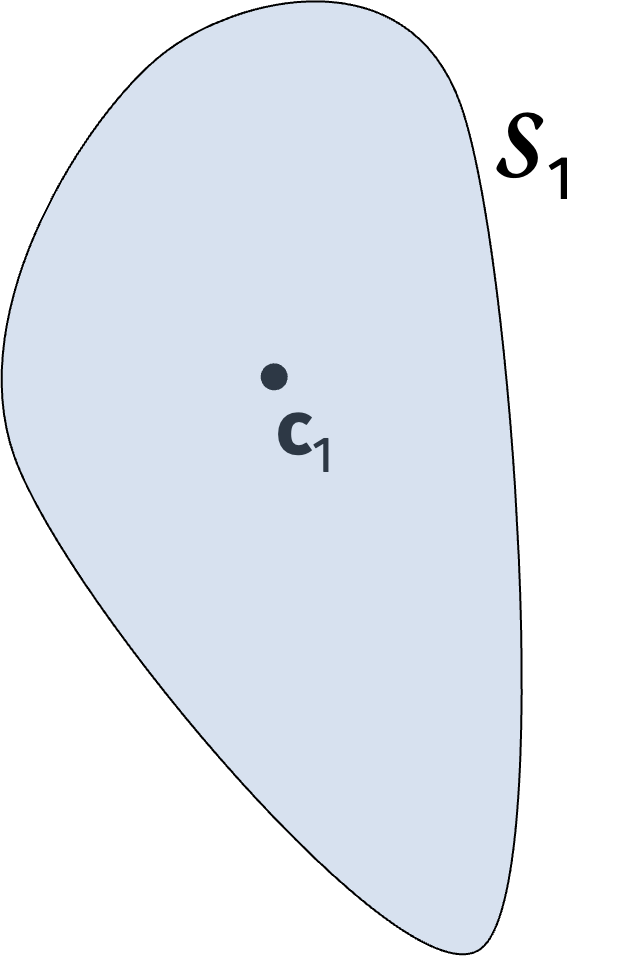
\includegraphics[width=\textwidth]{cog1.png}
\end{column}
\end{columns}
\end{frame}

\begin{frame}[t]
	\frametitle{center of gravity method}
	\begin{center}
		Natural ``cutting plane'' method.
	\end{center}
	\begin{columns}
		\begin{column}{.6\textwidth}
			\begin{itemize}
				\item $\mathcal{S}_1 = \mathcal{S}$
				\item For $t = 1, \ldots, T:$
				\begin{itemize}
					\item $\bv{c}_t = \text{center of gravity of } \mathcal{S}_t$.
					\item \alert{Compute $\nabla f(\bv{c}_t)$.}
					\item $\mathcal{H} = \{\bv{x} \big\vert \langle \nabla f(\bv{c}_t), \bv{x}-\bv{c}_t\rangle \leq 0\}$.
					\item $\mathcal{S}_{t+1} = \mathcal{S}_{t} \cap H$
				\end{itemize}
				\item Return $\hat{\mathbf{x}} = \argmin_t f(\bv{c}_t)$
			\end{itemize}
		\end{column}
		\begin{column}{.35\textwidth}
			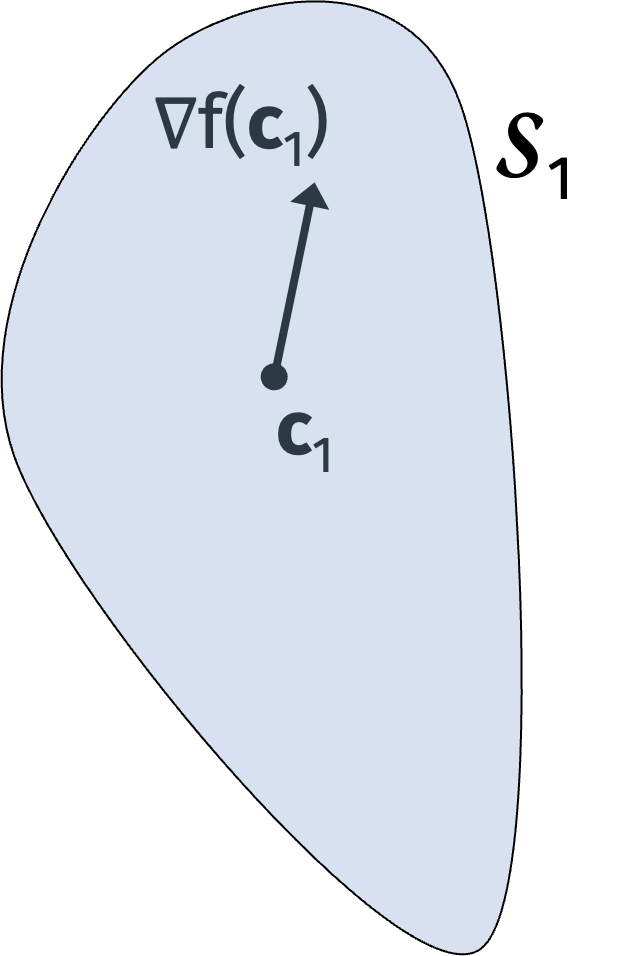
\includegraphics[width=\textwidth]{cog2.png}
		\end{column}
	\end{columns}
\end{frame}

\begin{frame}[t]
	\frametitle{center of gravity method}
	\begin{center}
		Natural ``cutting plane'' method.
	\end{center}
	\begin{columns}
		\begin{column}{.6\textwidth}
			\begin{itemize}
				\item $\mathcal{S}_1 = \mathcal{S}$
				\item For $t = 1, \ldots, T:$
				\begin{itemize}
					\item $\bv{c}_t = \text{center of gravity of } \mathcal{S}_t$.
					\item {Compute $\nabla f(\bv{c}_t)$.}
					\item \alert{$\mathcal{H} = \{\bv{x} \big\vert \langle \nabla f(\bv{c}_t), \bv{x}-\bv{c}_t\rangle \leq 0\}$.}
					\item \alert{$\mathcal{S}_{t+1} = \mathcal{S}_{t} \cap H$}
				\end{itemize}
				\item Return $\hat{\mathbf{x}} = \argmin_t f(\bv{c}_t)$
			\end{itemize}
		\end{column}
		\begin{column}{.6\textwidth}
			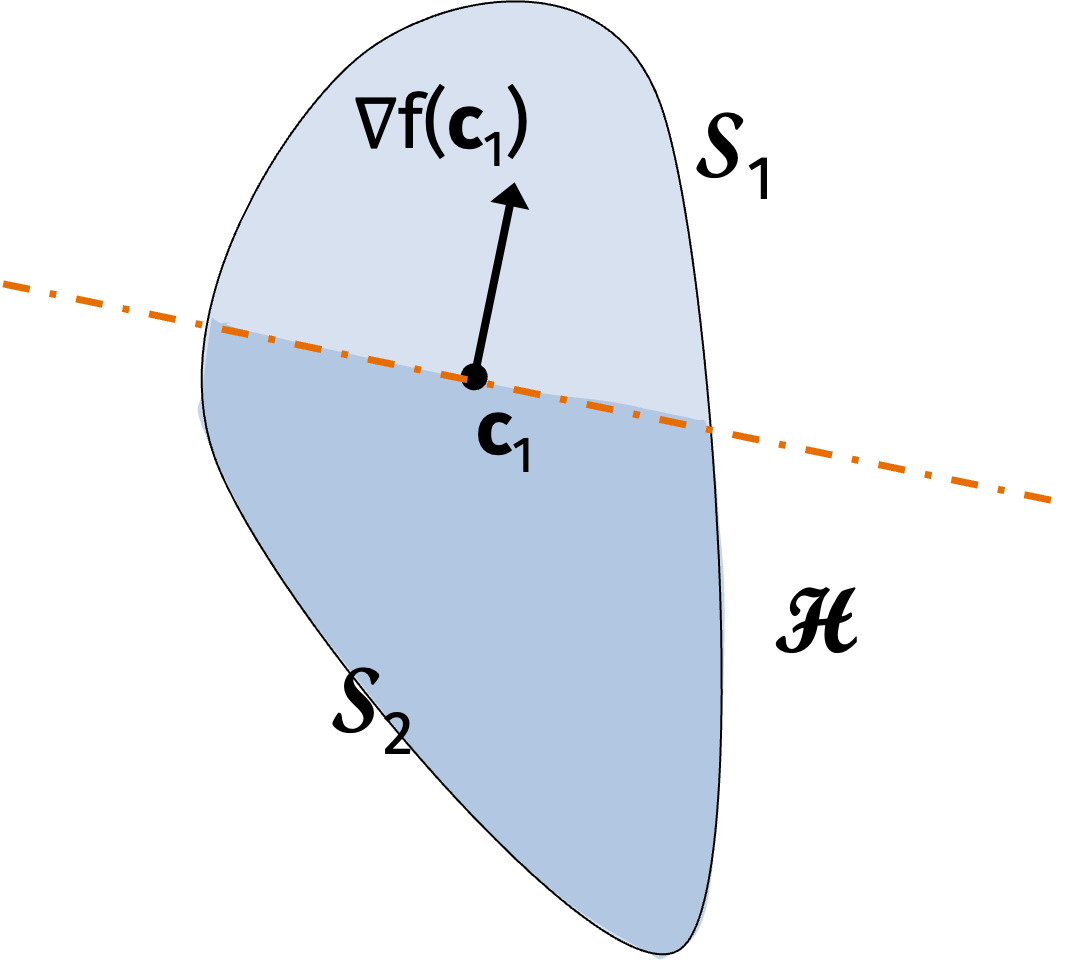
\includegraphics[width=\textwidth]{cog3.png}
		\end{column}
	\end{columns}
\end{frame}

\begin{frame}[t]
	\frametitle{center of gravity method}
	\textbf{Proof Reminder}:
	\begin{itemize}
		\item By Gr\"{u}nbaum's Theorem, cut the volume of the search space by a constant every step. 
		\item Need to reduce to a convex body whose volume is roughly $\epsilon^d$ smaller than the volume of $\mathcal{S}$.
		\item Final number of iterations scales with $\log(1/\epsilon^d)$
	\end{itemize}
\end{frame}

\begin{frame}[t]
		\frametitle{runtime issue}
		\textbf{In general computing the centroid is hard.} \#P-hard even when when $\mathcal{S}$ is an intersection of half-spaces (a polytope).
		
		Even if the problem isn't hard for your starting convex body $\mathcal{S}$, it likely will become hard for $\mathcal{S} \cap \mathcal{H}_1  \cap \mathcal{H}_2 \cap \mathcal{H}_3 \ldots$. 
		
		So while the \emph{oracle complexity} of dimension-dependent optimization was settled in the 60s, a number of basic questions in terms of \emph{computational complexity.}

		We will see how to resolve this issue with an elegant cutting plane methods called the \textbf{Ellipsoid Method} that was introduced by Naum Shor in 1977.
\end{frame}

\begin{frame}[t]
	\frametitle{problem simplification}
	\small
		\textbf{Slightly more general problem:}
		Given a convex set $\mathcal{K}$ via access to \emph{separation oracle} $S_\mathcal{K}$ for the set, determine if $\mathcal{K}$ is empty, or otherwise return any point $\bv{x}\in \mathcal{K}$. 
		\vspace{-2em}
		
		\begin{align*}
			\bv{S}_k(\bv{y}) = \begin{cases}
				\emptyset &\text{ if } \bv{y} \in \mathcal{K}. \\
				\text{separating hyperplane } (\bv{a},c) &\text{ if } \bv{y} \notin \mathcal{K}.
			\end{cases}
		\end{align*}
	
	Let $\mathcal{H} = \{\bv{x}: \bv{a}^T\bv{x} = c\}$.
	\vspace{-1em}
		\begin{center}
			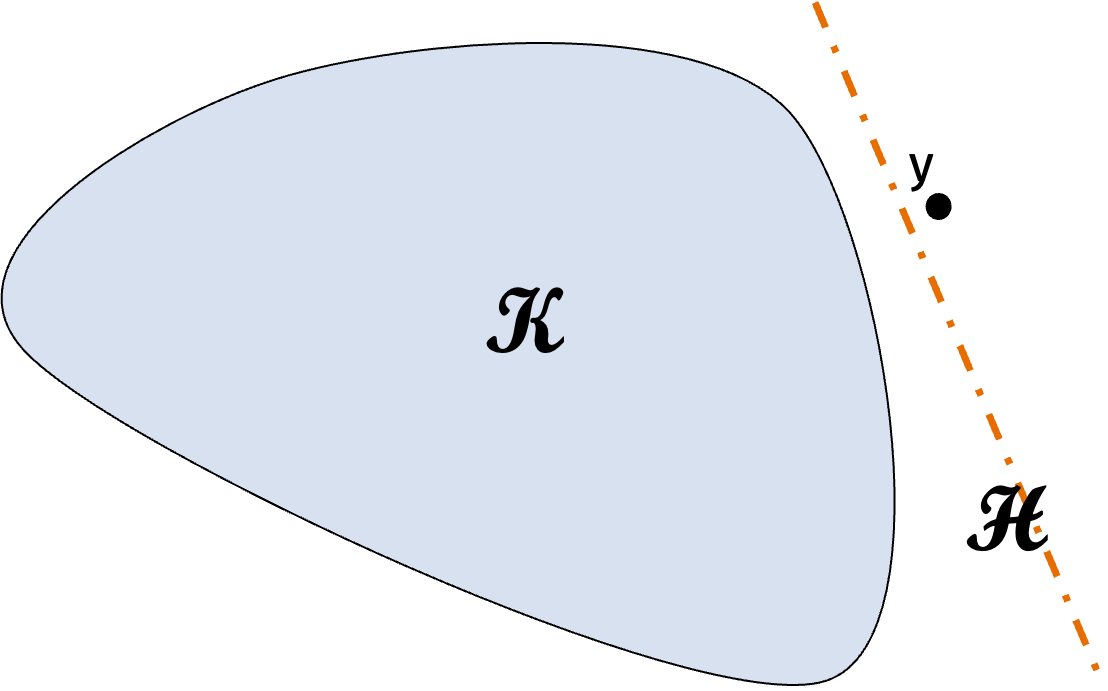
\includegraphics[width=.65\textwidth]{seperationoracle.png}
		\end{center}
	
\end{frame}

\begin{frame}[t]
	\frametitle{separation oracle}
	\textbf{Example:} How would you implement a separation oracle for a polytope $\{\bv{x}: \bv{A}\bv{x} \geq \bv{b}\}$. 
\end{frame}

\begin{frame}[t]
	\frametitle{from membership to optimization}
	\textbf{Original problem:} $\min_{\bv{x}\in \mathcal{S}} f(\bv{x})$.

	How to reduce to determining if a convex set $\mathcal{K}$ is empty or not?
	\begin{center}
	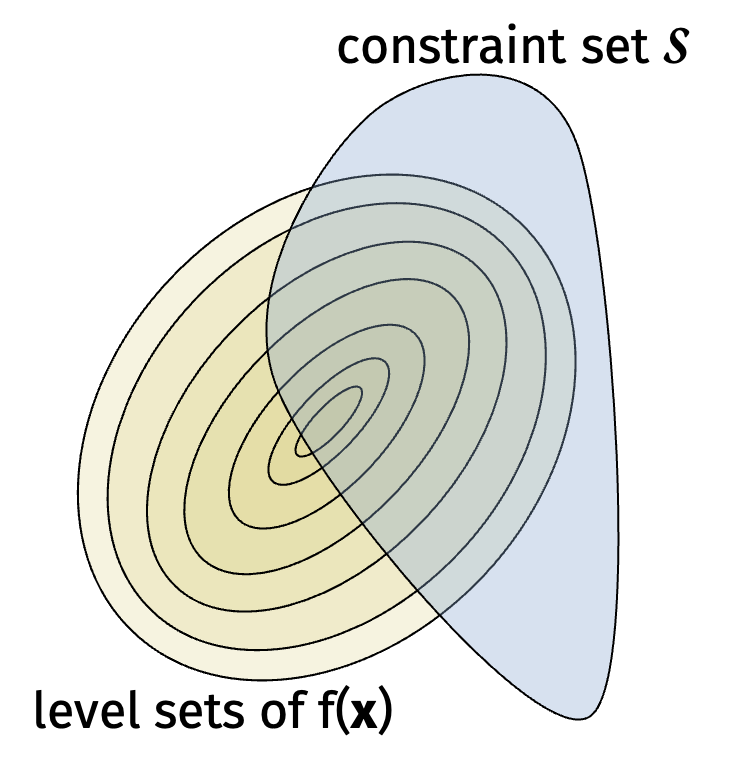
\includegraphics[width=.5\textwidth]{level_sets_constrained.png}
	\end{center}
	
\end{frame}

\begin{frame}[t]
	\frametitle{from membership to optimization}
	\textbf{Original problem:} $\min_{\bv{x}\in \mathcal{S}} f(\bv{x})$.

	How to reduce to determining if a convex set $\mathcal{K}$ is empty or not?
	\begin{center}
		\vspace{-1em}
	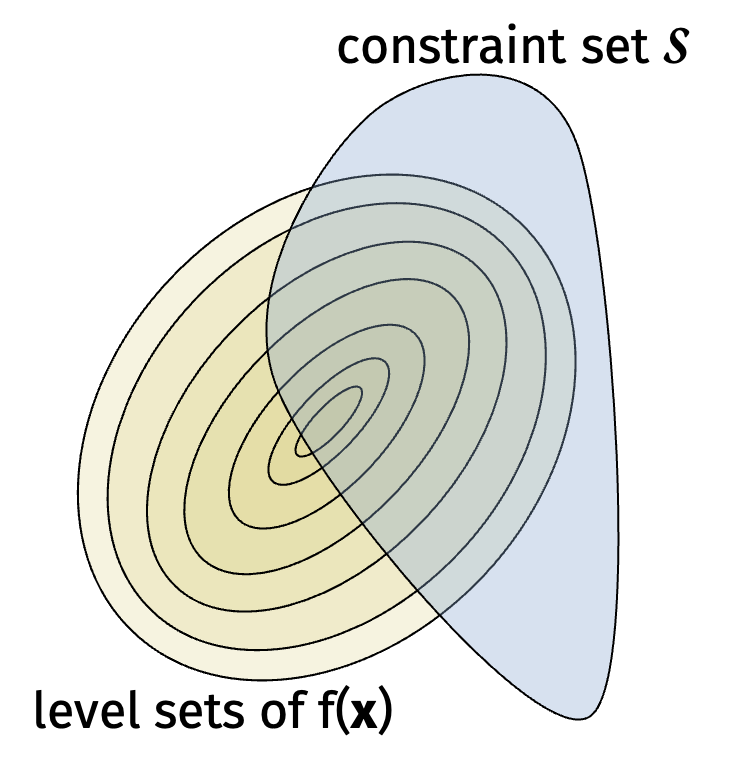
\includegraphics[width=.5\textwidth]{level_sets_constrained.png}
	\vspace{-1em}
	\end{center}
	
	\textbf{Binary search!} For a convex function $f(\bv{x})$, $\{\bv{x}: f(\bv{x}) \leq c\}$ is convex, and you can get a separation oracle via the gradient.
\end{frame}



\begin{frame}[t]
\frametitle{ellipsoid method sketch}
\textbf{Goal of ellipsoid algorithm:} Solve ``Is $\mathcal{K}$ empty or not?" given a separation oracle for $\mathcal{K}$ under the assumptions that:
\begin{enumerate}
	\item $\mathcal{K} \subset B(\bv{c}_R, R)$.
	\item If non-empty, $\mathcal{K}$ contains $B(\bv{c}_r, r)$ for some $r < R$. 
\end{enumerate}
\begin{center}
	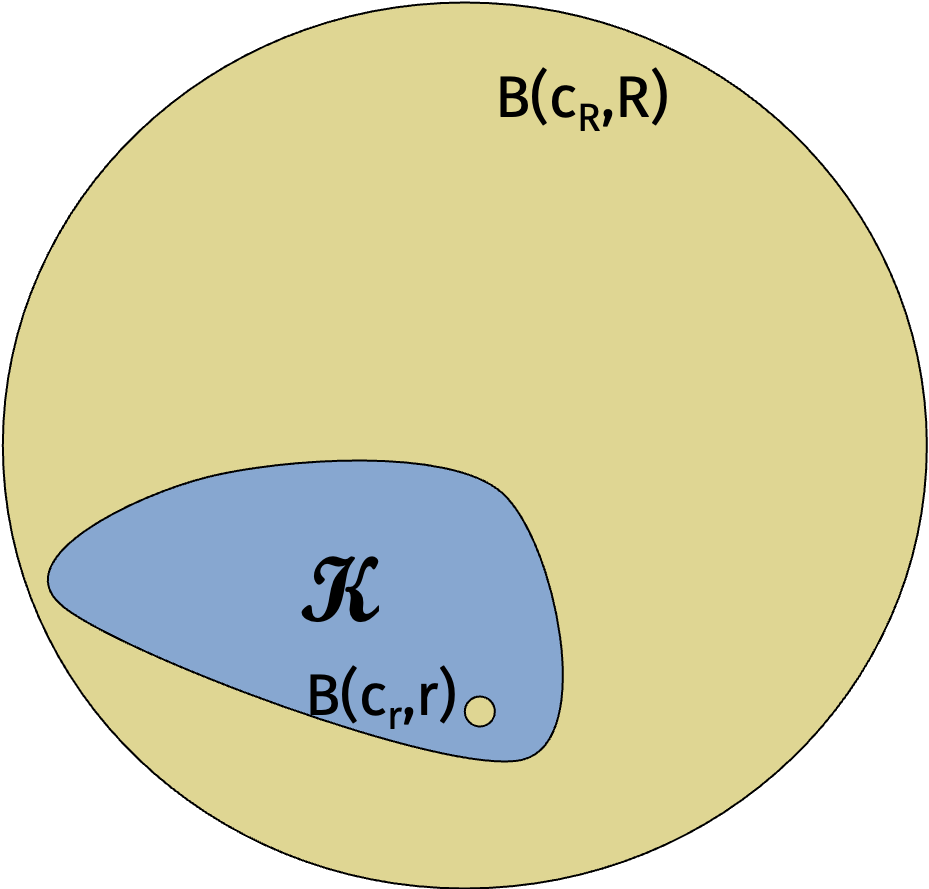
\includegraphics[width=.5\textwidth]{ellipsoid0.png}
\end{center}
\end{frame}

\begin{frame}[t]
	\frametitle{ellipsoid method sketch}
	\begin{center}
		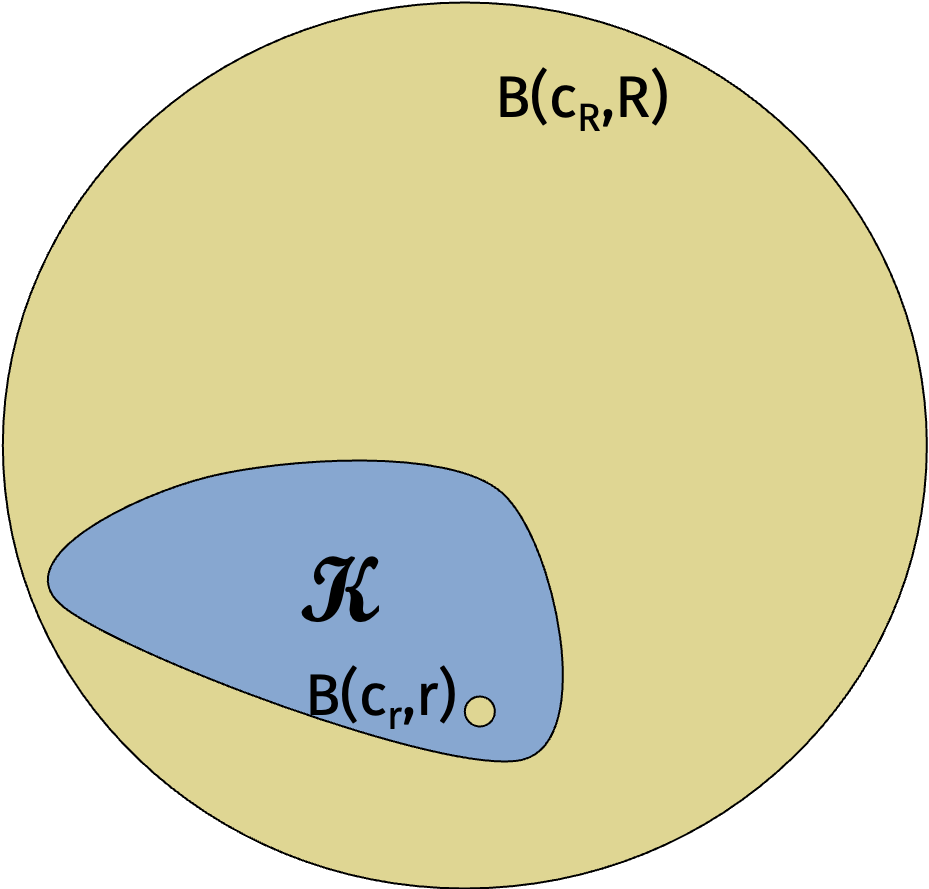
\includegraphics[width=.5\textwidth]{ellipsoid0.png}
	\end{center}
	\textbf{Application to original problem:} For a convex function $f$ such that $\|\nabla f(\bv{x})\|_2 \leq G$, it can be checked that the convex set $\{\bv{x} : f(\bv{x}) \leq \epsilon\}$ contains a ball of radius $\epsilon/G$. 
	\end{frame}
	

\begin{frame}[t]
	\frametitle{ellipsoid method sketch}
	Iterative method similar to center-of-gravity:
	\begin{enumerate}
		\item Check if center $\bv{c}_R$ of $B(\bv{c}_R, R)$ is in $\mathcal{K}$.
		\item If it is, we are done.
		\item  If not, cut search space in half, using separating hyperplane. 
	\end{enumerate}
	\begin{center}
		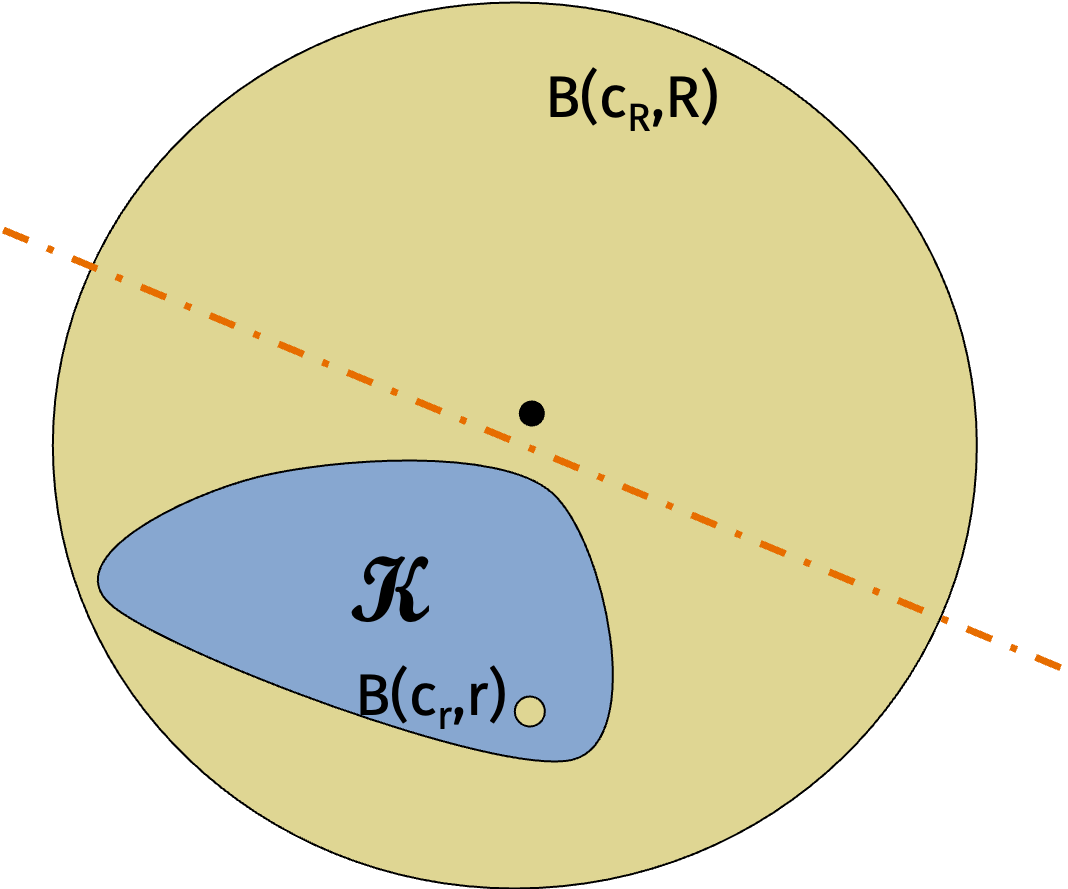
\includegraphics[width=.5\textwidth]{ellipsoid1.png}
	\end{center}
\end{frame}

\begin{frame}[t]
	\frametitle{ellipsoid method sketch}
	\textbf{Key insight:} Before moving on, approximate new search region by something that we can easily compute the centroid of. Specifically an ellipse!
	\vspace{-1em}
	\begin{center}
		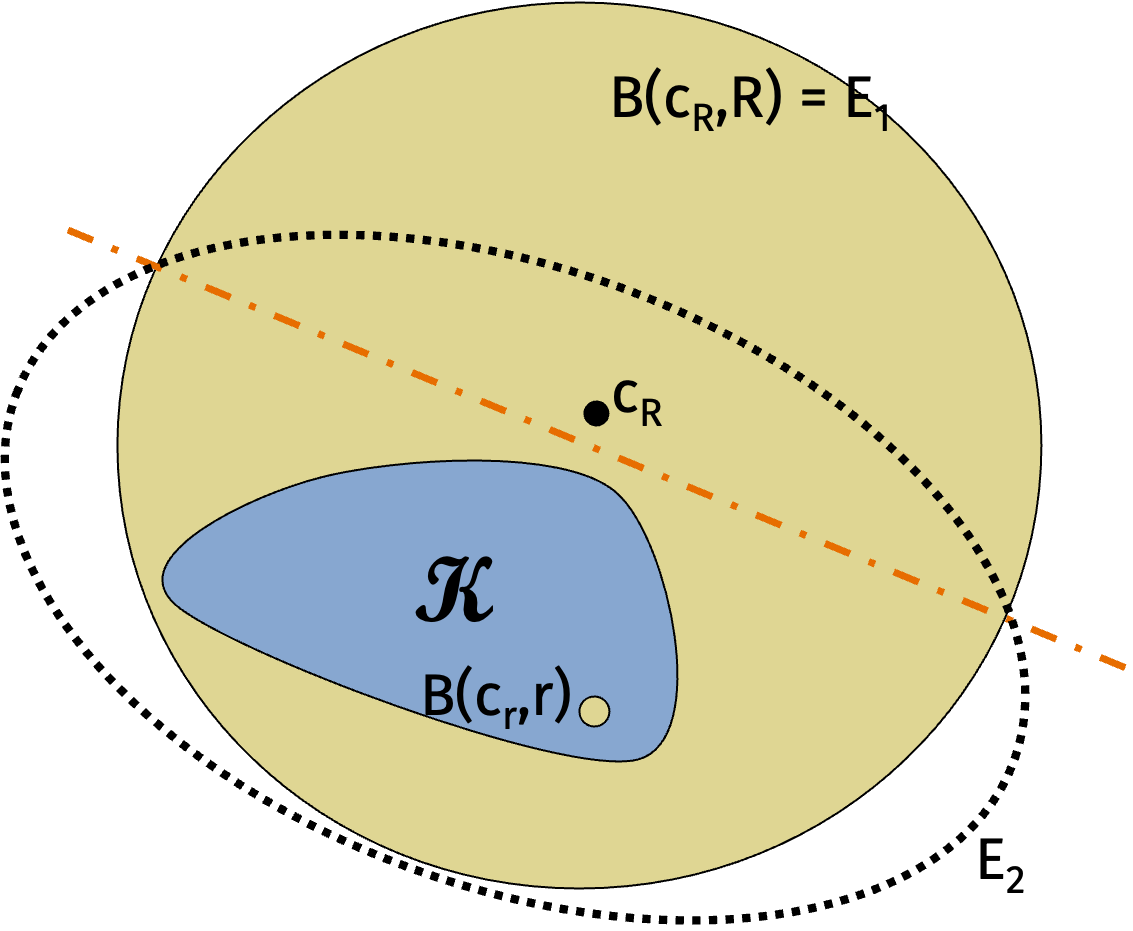
\includegraphics[width=.5\textwidth]{ellipsoid2.png}
	\end{center}
	\vspace{-1em}
Produce a sequence of ellipses that \emph{always contain} $\mathcal{K}$ and decrease in volume: $B(\bv{c}_R, R) = E_1, E_2, \ldots$. Once we get to an ellipse with volume $\leq B(\bv{c}_r, r)$, we know that $\mathcal{K}$ must be empty.
\end{frame}

\begin{frame}
		\frametitle{ellipse}
		An ellipse is a convex set of the form: $\{\bv{x}: \|\bv{A}(\bv{x} - \bv{c})\|_2^2 \leq \alpha\}$ for some constant $c$ and matrix $\bv{A}$. The center-of-mass is  $\bv{c}$. 
		\begin{center}
			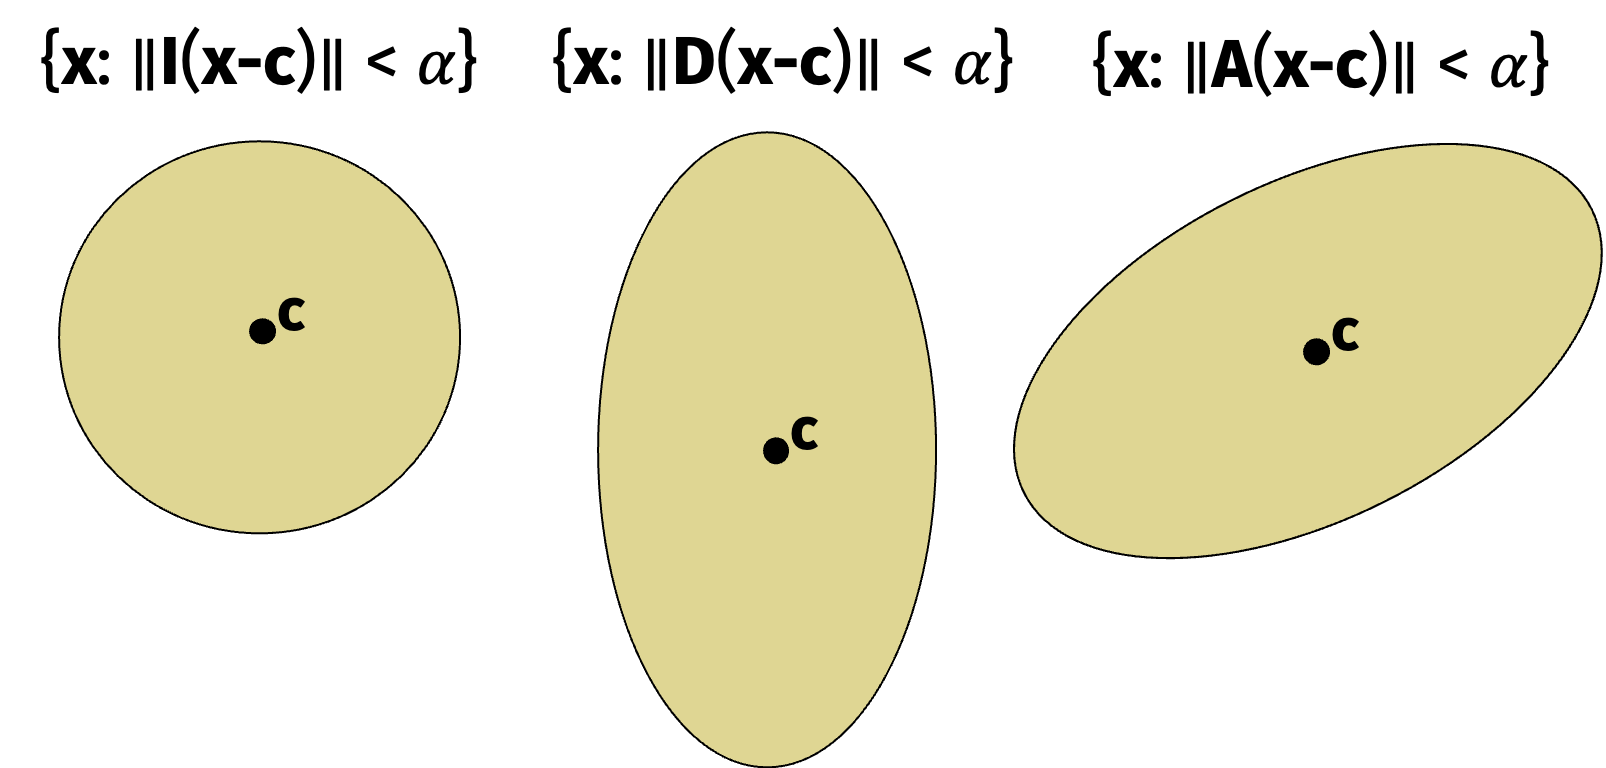
\includegraphics[width=\textwidth]{ellipses.png}
		\end{center}
	
	Often re-parameterized to say that the ellipse is all $\bv{x}$ with $\{\bv{x}: (\bv{x} - \bv{c})^T\bv{Q}^{-1}(\bv{x} - \bv{c})\leq 1\}$
\end{frame}

\begin{frame}
	\frametitle{ellipsoid update}
	There is a closed form solution for the equation of the smallest ellipse containing a given half-ellipse. I.e. let $\bv{E}_i$ have parameters $\bv{Q}_i,\bv{c}_i$ and consider the half-ellipse:
	\begin{align*}
		\bv{E}_i \cap \{\bv{x}: \bv{a}_i^T\bv{x} \leq \bv{a}_i^T\bv{c}_i\}. 
	\end{align*}
Then $\bv{E}_{i+1}$ is the ellipse with parameters:
\begin{align*}
	\bv{Q}_{i+1} &= \frac{d^2}{d^2 - 1}\left(\bv{Q}_{i} - \frac{2}{d+1} \bv{h}\bv{h}^T \right) & \bv{c}_{i+1}& = \bv{c}_{i} - \frac{1}{n+1}\bv{h},
\end{align*}
where $\bv{h} = \sqrt{\bv{a}_i^T\bv{Q}_i\bv{a}_i}\cdot \bv{a}_i$.

\textbf{\alert{Computing the update takes $O(d^2)$ time.}}
	
\end{frame}


\begin{frame}[t]
	\frametitle{geometric observation}
	\textbf{Claim:} $\vol(E_{i+1}) \leq (1-\frac{1}{2d})\vol(E_i)$.
	
	\textbf{Proof:} Via reduction to the ``isotropic case''. I will post a proof on the course website if you are interested. 
	\vspace{-.5em}
	\begin{center}
		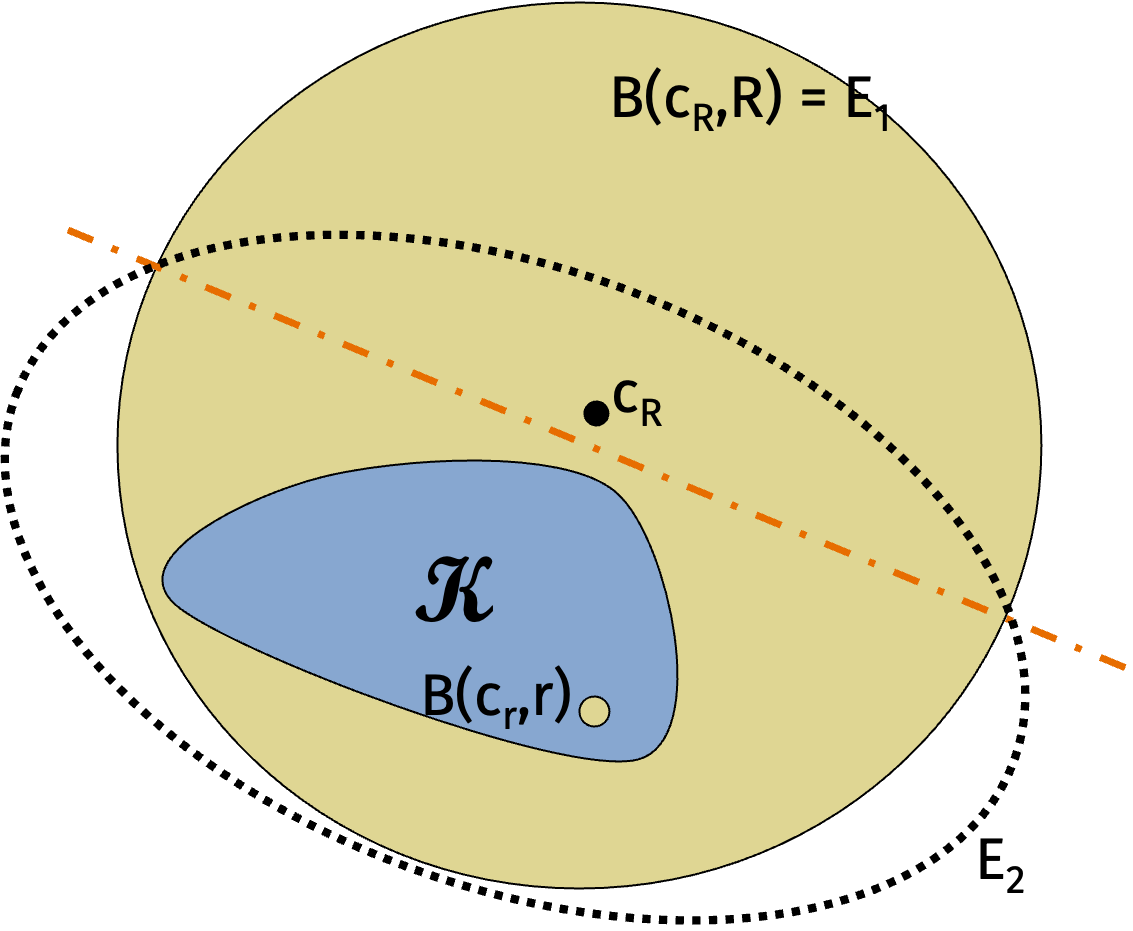
\includegraphics[width=.5\textwidth]{ellipsoid2.png}
	\end{center}
	\vspace{-.5em}
Not as good as the $(1-\frac{1}{e})$ constant-factor volume reduction we got from center-of-gravity, but still very good! 
\end{frame}


\begin{frame}[t]
	\frametitle{geometric observation}
	\textbf{Claim:} $\vol(E_{i+1}) \leq (1-\frac{1}{2d})\vol(E_i)$

	\begin{center}
		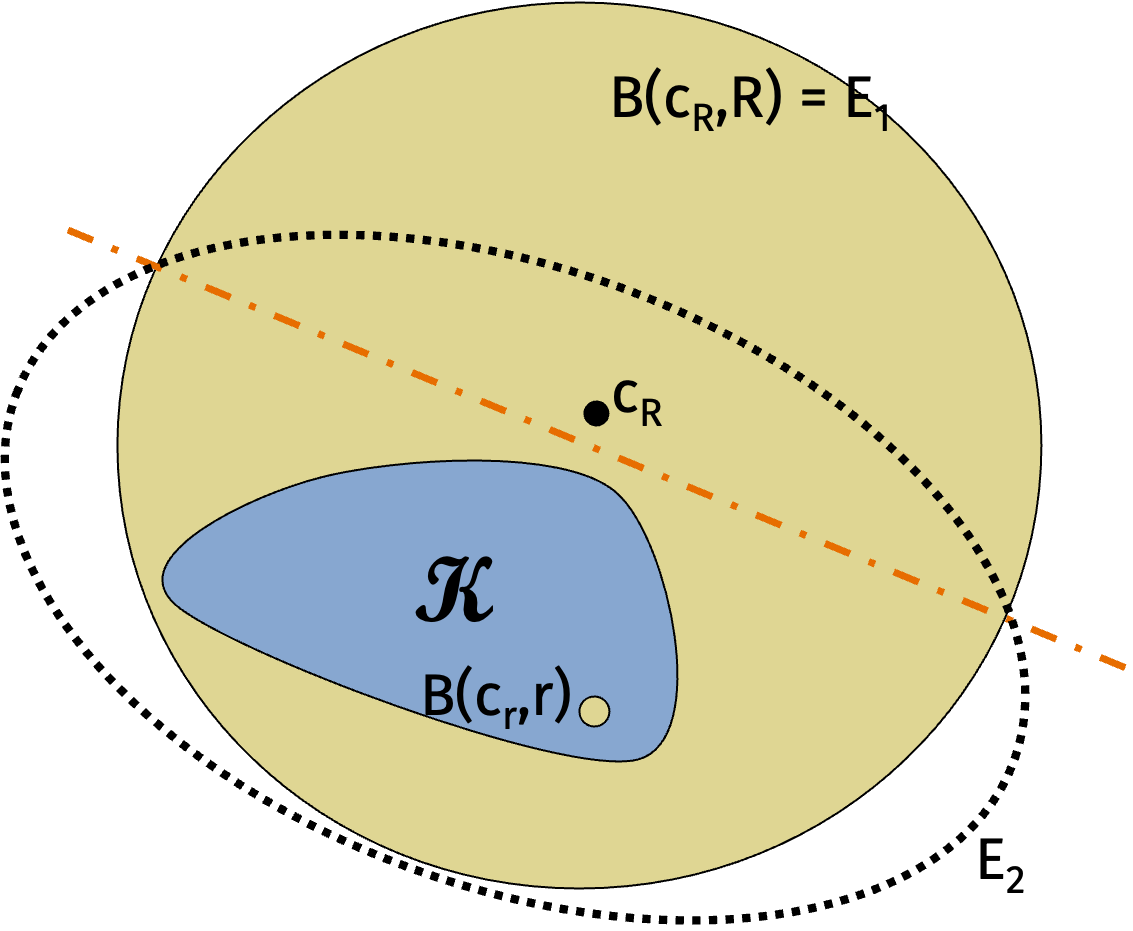
\includegraphics[width=.5\textwidth]{ellipsoid2.png}
	\end{center}
	\begin{center}
		After $O(d)$ iterations, we reduce the volume by a constant.
		
		In total require $O(d^2\log(R/r))$ iterations to solve the problem.
	\end{center}
\end{frame}

\begin{frame}[t]
	\frametitle{linear programming}
	\textbf{Linear programs} (LPs) are one of the most basic convex constrained, convex optimization problems:
	
	Let $\bv{c}\in \R^d, \bv{b}\in \R^n, \bv{A}\in \R^{n\times d}$ be fixed vectors that define the problem, and let $\bv{x}$ be our variable parameter.
	\begin{align*}
	\min f(\bv{x}) &= \bv{c}^T\bv{x}\\
	\text{subject to } \bv{A}\bv{x} &\geq \bv{b}.
	\end{align*}
	
Think about $\bv{A}\bv{x} \geq \bv{b}$ as a union of half-space constraints:
\begin{align*}
	&\{\bv{x}: \bv{a}_1^T\bv{x} \geq {b}_1 \}\\
		&\{\bv{x}: \bv{a}_2^T\bv{x} \geq {b}_2 \}\\
			&\hspace{2.3em}\vdots\\
			&\{\bv{x}: \bv{a}_n^T\bv{x} \geq {b}_n \}
\end{align*}
	
\end{frame}

\begin{frame}[t]
	\frametitle{killer application: linear programming}
	\begin{align*}
		\min f(\bv{x}) &= \bv{c}^T\bv{x}\\
		\text{subject to } \bv{A}\bv{x} &\geq \bv{b}.
	\end{align*}
	
	\begin{center}
		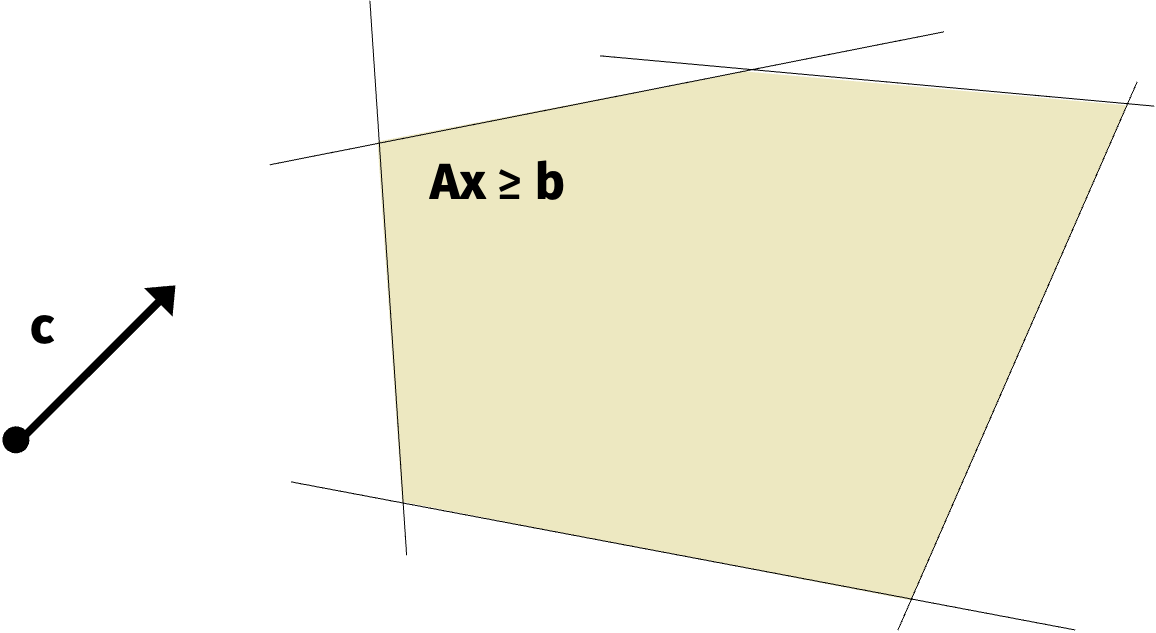
\includegraphics[width=.8\textwidth]{lpexample.png}
	\end{center}
\end{frame}

\begin{frame}
		\frametitle{linear programming applications}
	\begin{itemize}
		\item Classic optimization applications: industrial resource optimization problems were killer app in the 70s.
		\item Robust regression: $\min_{\bv{x}} \|\bv{A} \bv{x} - \bv{b}\|_1$. 
		\item $L1$ constrained regression: $\min_{\bv{x}} \|\bv{x}\|_1$ subject to $\bv{A}\bv{x} = \bv{b}$. Lots of applications in sparse recovery/compressed sensing.
		\item Solve $\min_{\bv{x}}\|\bv{A} \bv{x} - \bv{b}\|_{\infty}$.   
		\item Polynomial time algorithms for Markov Decision Processes. 
		\item \alert{\textbf{Many combinatorial optimization problems can be solved via \emph{LP relaxations}.}}
	\end{itemize}
\end{frame}

\begin{frame}[t]
	\frametitle{linear programming}
	\begin{theorem}[Khachiyan, 1979]
	Assume $n=d$. The \emph{ellipsoid method} solves any linear program with $L$-bit integer valued constraints \emph{exactly} in $O(n^4L)$ time. 
	\end{theorem}
	\begin{center}
		
\includegraphics[width=\textwidth]{ellipsoidnews.png}
		Front page of New York Times, November 9, 1979.
	\end{center}
\end{frame}

\begin{frame}[t]
	\frametitle{interior point methods}
	\begin{theorem}[Karmarkar, 1984]
		Assume $n=d$. The \emph{interior point method} solves any linear program with $L$-bit integer valued constraints in $O(n^{3.5}L)$ time. 
	\end{theorem}
	\begin{center}
	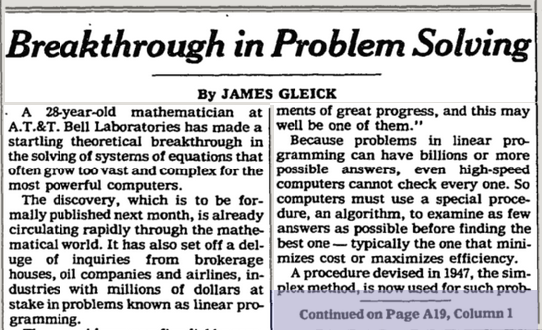
\includegraphics[width=.7\textwidth]{interiornews.png}
	
			Front page of New York Times, November 19, 1984.
	\end{center}
\end{frame}

\begin{frame}[t]
	\frametitle{interior point methods}
	Lecture notes are posted on the website (optional reading).
	\begin{center}
			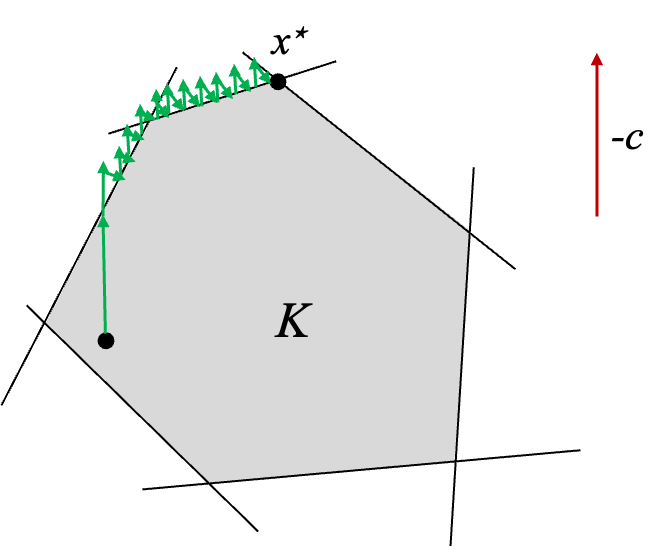
\includegraphics[width=.6\textwidth]{projected_gradient.png}
			
			Projected Gradient Descent Optimization Path
	\end{center}

\end{frame}

\begin{frame}[t]
	\frametitle{interior point methods}
	Lecture notes are posted on the website (optional reading).
	\begin{center}
		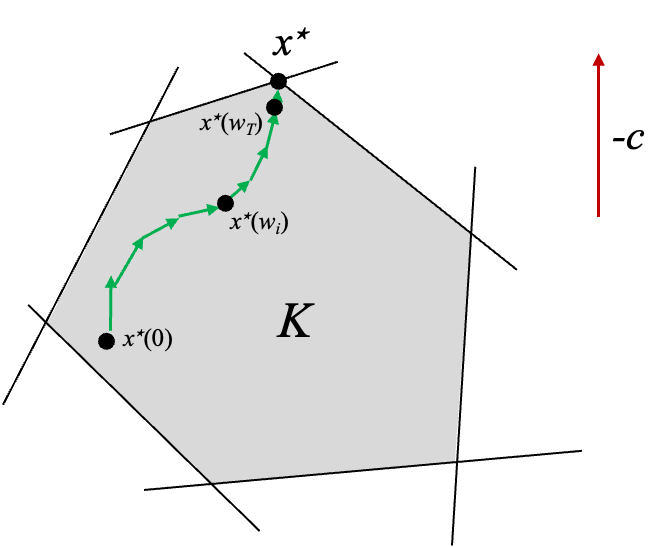
\includegraphics[width=.6\textwidth]{interior_point.png}
		
		Ideal Interior Point Optimization Path
	\end{center}
	
\end{frame}

\begin{frame}[t]
	\frametitle{polynomial time linear programming}
	Both results had a huge impact on the theory of optimization, although at the time neither the ellipsoid method or interior point method were faster than a heuristic known at the Simplex Method. 
	
	These days, improved interior point methods compete with and often outperform simplex.

	Polynomial time linear programming algorithms have also had a huge impact of \emph{combinatorial optimization.} They are often the work-horse behind approximation algorithms for NP-hard problems.  
\end{frame}

\begin{frame}[t]
	\frametitle{example: vertex cover}
	Given a graph $G$ with $n$ nodes and edge set $E$. Each node is assigned a weight $w_1, \ldots, w_n$.
	\begin{center}
		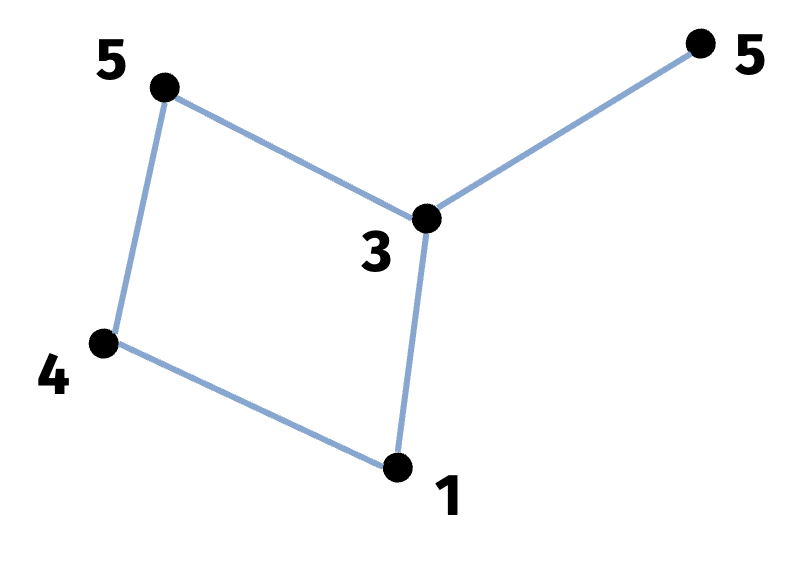
\includegraphics[width=.6\textwidth]{vertex_cover.png}
	\end{center}
	\textbf{Goal:} Select subset of nodes with minimum total weight that covers all edges.
\end{frame}

\begin{frame}[t]
	\frametitle{example: vertex cover}
	Given a graph $G$ with $n$ nodes and edge set $E$. Each node is assigned a weight $w_1, \ldots, w_n$.

	\textbf{Formally:} Denote if node $i$ is selected by assigning variable $x_i$ to $0$ or $1$. Let $\bv{x} = [x_1, \ldots, x_n]$.
	\begin{align*}
		\min_{\bv{x}} &\sum_{i=1}^n x_i w_i & &\text{subject to} & x_i &\in \{0,1\} \text{ for all $i$}\\
		&&&& x_i + x_j &\geq 1 \text{ for all } (i,j) \in E
	\end{align*}

	\textbf{NP-hard to solve exactly.} We will use convex optimization give a $2$-approximation in polynomial time.

	Function to minimize is linear (so convex) but constraint set is not convex. Why?
\end{frame}

\begin{frame}[t]
	\frametitle{relax-and-round}
	\textbf{High level approach}: 
	\begin{itemize}
		\item \emph{Relax} to a problem with convex constraints. 
		\item \emph{Round} optimal solution of convex problem back to original constraint set.
	\end{itemize}
	\begin{center}
		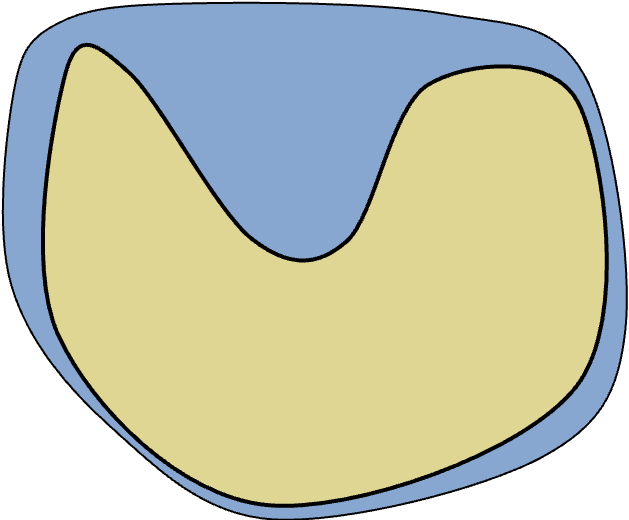
\includegraphics[width=.5\textwidth]{relaxround1.png}
	\end{center}
\end{frame}

\begin{frame}[t]
	\frametitle{relax-and-round}
	\textbf{High level approach}: 
	\begin{itemize}
		\item \emph{Relax} to a problem with convex constraints. 
		\item \emph{Round} optimal solution of convex problem back to original constraint set.
	\end{itemize}
	\begin{center}
		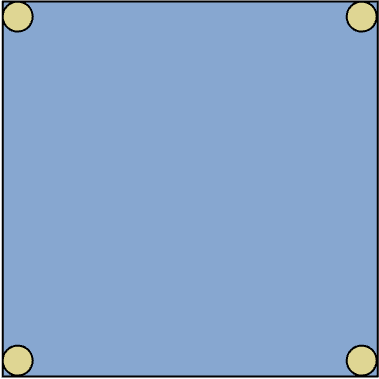
\includegraphics[width=.4\textwidth]{relaxround2.png}
	\end{center}
\end{frame}

\begin{frame}[t]
	\frametitle{relax-and-round}
	\textbf{High level approach}: 
	\begin{itemize}
		\item \emph{Relax} to a problem with convex constraints. 
		\item \emph{Round} optimal solution of convex problem back to original constraint set.
	\end{itemize}
Let $\bar{\mathcal{S}} \supseteq \mathcal{S}$ be the relaxed constraint set. Let $\bv{x}^* = \argmin_{\bv{x}\in \mathcal{S}} f(\bv{x})$ and let $\bar{\bv{x}}^* = \argmin_{\bv{x}\in \bar{\mathcal{S}}} f(\bv{x})$. We always have that:
\begin{align*}
	f(\bar{\bv{x}}^*) \leq f(\bv{x}^*). 
\end{align*}
So typically the goal is to round $\bar{\bv{x}}^*$ to $\mathcal{S}$ in such a way that we don't increase the function value too much.
\end{frame}

\begin{frame}[t]{relaxing vertex cover}
\textbf{Vertex Cover:}
	\begin{align*}
		\min_{\bv{x}} &\sum_{i=1}^n x_i w_i & &\text{subject to} & \alert{x_i} &\alert{\in \{0,1\}} \text{ for all $i$}\\
		&&&& x_i + x_j &\geq 1 \text{ for all } (i,j) \in E
	\end{align*}

\textbf{Relaxed Vertex Cover:}
\begin{align*}
	\min_{\bv{x}} &\sum_{i=1}^n x_i w_i & &\text{subject to} & \alert{0} &\alert{\leq x_i \leq 1} \text{ for all $i$}\\
	&&&& x_i + x_j &\geq 1 \text{ for all } (i,j) \in E
\end{align*}
The second problem is a linear program! It can be solved in $\poly(n)$ time! 
\end{frame}

\begin{frame}[t]{rounding vertex cover}
	Simply set all variable $x_i = 1$ of $\bar{x}_i^* \geq 1/2$ and $x_i = 0$ otherwise.
	\begin{center}
		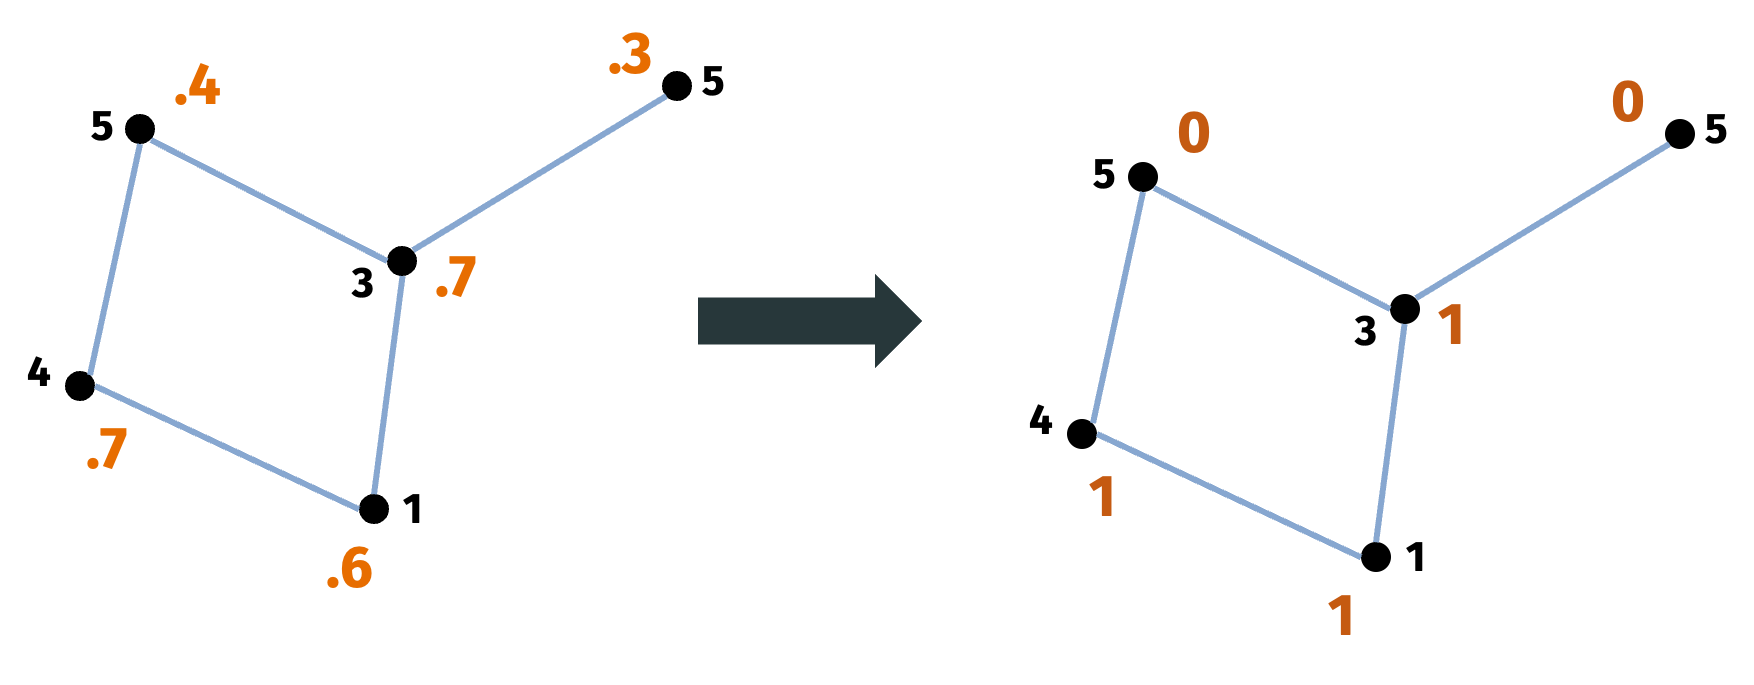
\includegraphics[width=\textwidth]{round.png}
	\end{center}
	\textbf{Observation 1:} All edges remain covered. I.e., the constraint $x_i + x_j \geq 1 \text{ for all } (i,j) \in E$ is not violated.
\end{frame}

\begin{frame}[t]{rounding vertex cover}
	\textbf{Observation 2:} Let $\bv{x}$ be the rounded version of $\bar{\bv{x}}^*$. We have $f(\bv{x}) \leq 2 \cdot f(\bar{\bv{x}})$, and thus $f(\bv{x}) \leq 2 \cdot f({\bv{x}^*})$. 

	\textbf{Proof:}

\end{frame}

\begin{frame}[t]{vertex cover}
	So, a polynomial time algorithm for solving LPs immediately yields a $2$-approximation algorithm for the NP-hard problem of vertex cover. 

	\begin{itemize}
		\item Proven that it is NP-hard to do better than a $1.36$ approximation in [Dinur, Safra, 2002]. 
		\item Recently improved to $\sqrt{2} \approx 1.41$ in [Khot, Minzer, Safra 2018], which proved the 2-to-2 games conjecture. 
		\item Widely believed that doing better than $2-\epsilon$ is NP-hard for any $\epsilon > 0$, and this is implied by Subhash Khot's Unique Games Conjecture.
	\end{itemize}
	There is a simpler greedy 2-approximation algorithm that doesn't use optimization at all. Try coming up with it on your own!
\end{frame}

\begin{frame}[standout]
	\begin{center}
			\large break
		\end{center}
\end{frame}

\begin{frame}{spectral methods}
	\textbf{Next section of course:} \emph{Spectral methods} and \emph{numerical linear algebra}.

	Spectral methods generally refer to methods based on the ``spectrum'' of a matrix. I.e. on it's eigenvectors/eigenvalues and singular vectors/singular values. We will look at applications in:
	\begin{itemize}
		\item Low-rank approximation and dimensionality reduction.
		\item Data clustering and related problems.
		\item Constructing data embeddings (e.g. Word2Vec).
	\end{itemize}
\end{frame}

\begin{frame}{spectral methods}
	\textbf{Reminder:} A vector $\bv{v}\in \R^{d}$ is an \emph{eigenvector} of a matrix $\bv{X}\in \R^{d\times d}$, if there exists a scalar $\lambda$ such that 
	\begin{align*}
		\bv{X}\bv{v} = \lambda \bv{v}
	\end{align*}
	The scalar $\lambda$ is called the \emph{eigenvalue} associated with $\bv{v}$.

	Matrices can often be written completely in terms of their eigenvectors and eigenvalues. This is called eigendecomposition. 

	We will actually focus on a related tool called \emph{singular value decomposition.}
\end{frame}



%\begin{frame}
%	\frametitle{spectral methods}
%	\textbf{Return to data compression}:
%	\begin{center}
%		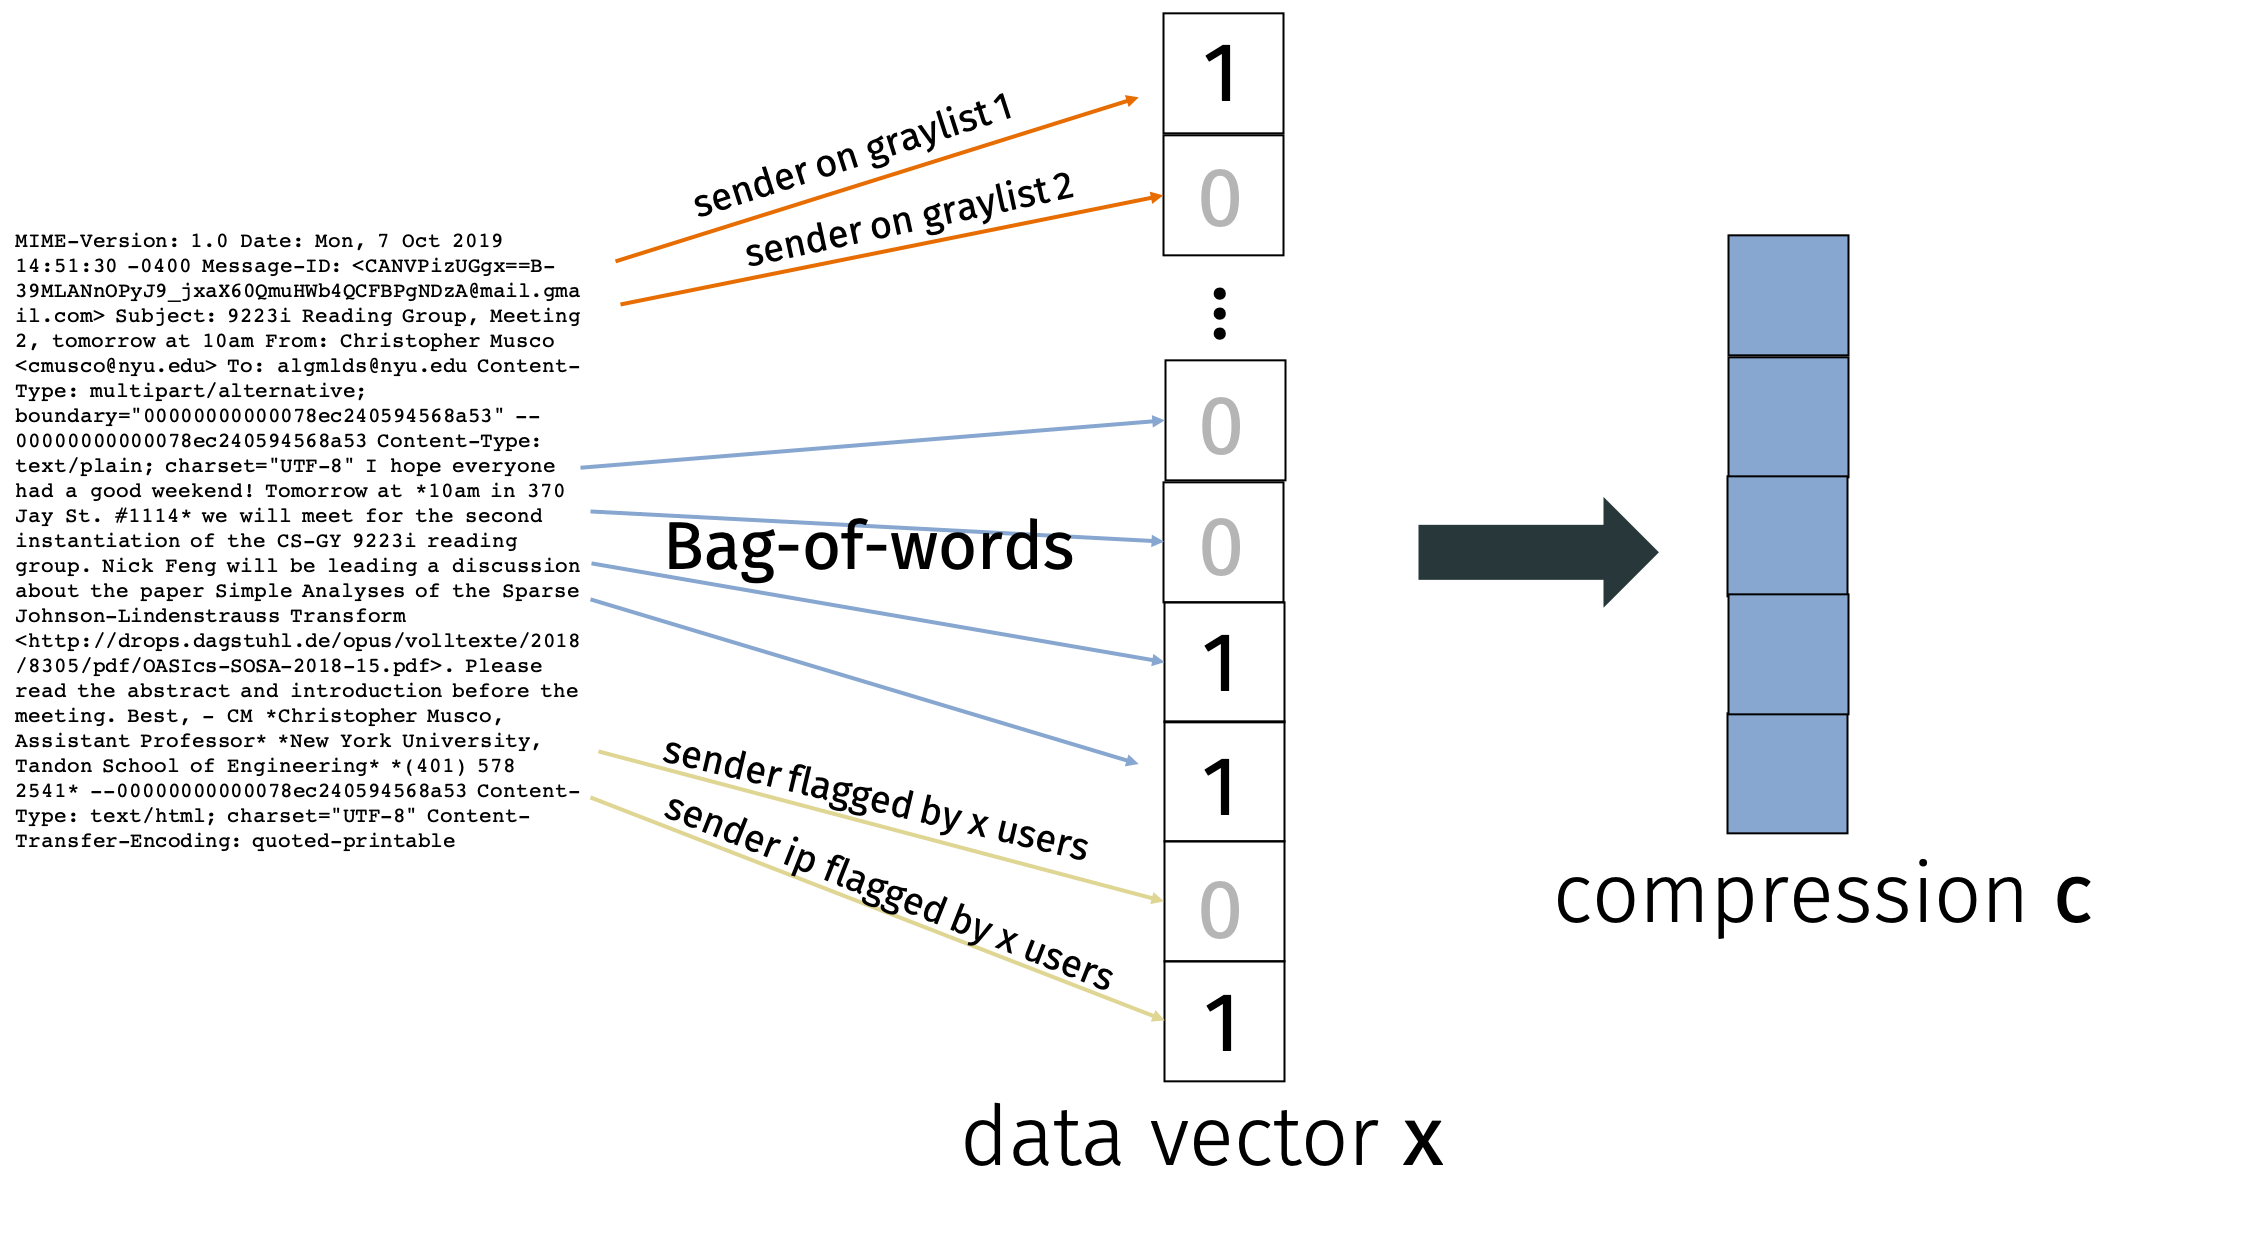
\includegraphics[width=.8\textwidth]{bow.png}
%	\end{center}
%\end{frame}

%\begin{frame}
%	\frametitle{spectral methods}
%	\textbf{Return to data compression}:
%	\begin{center}
%		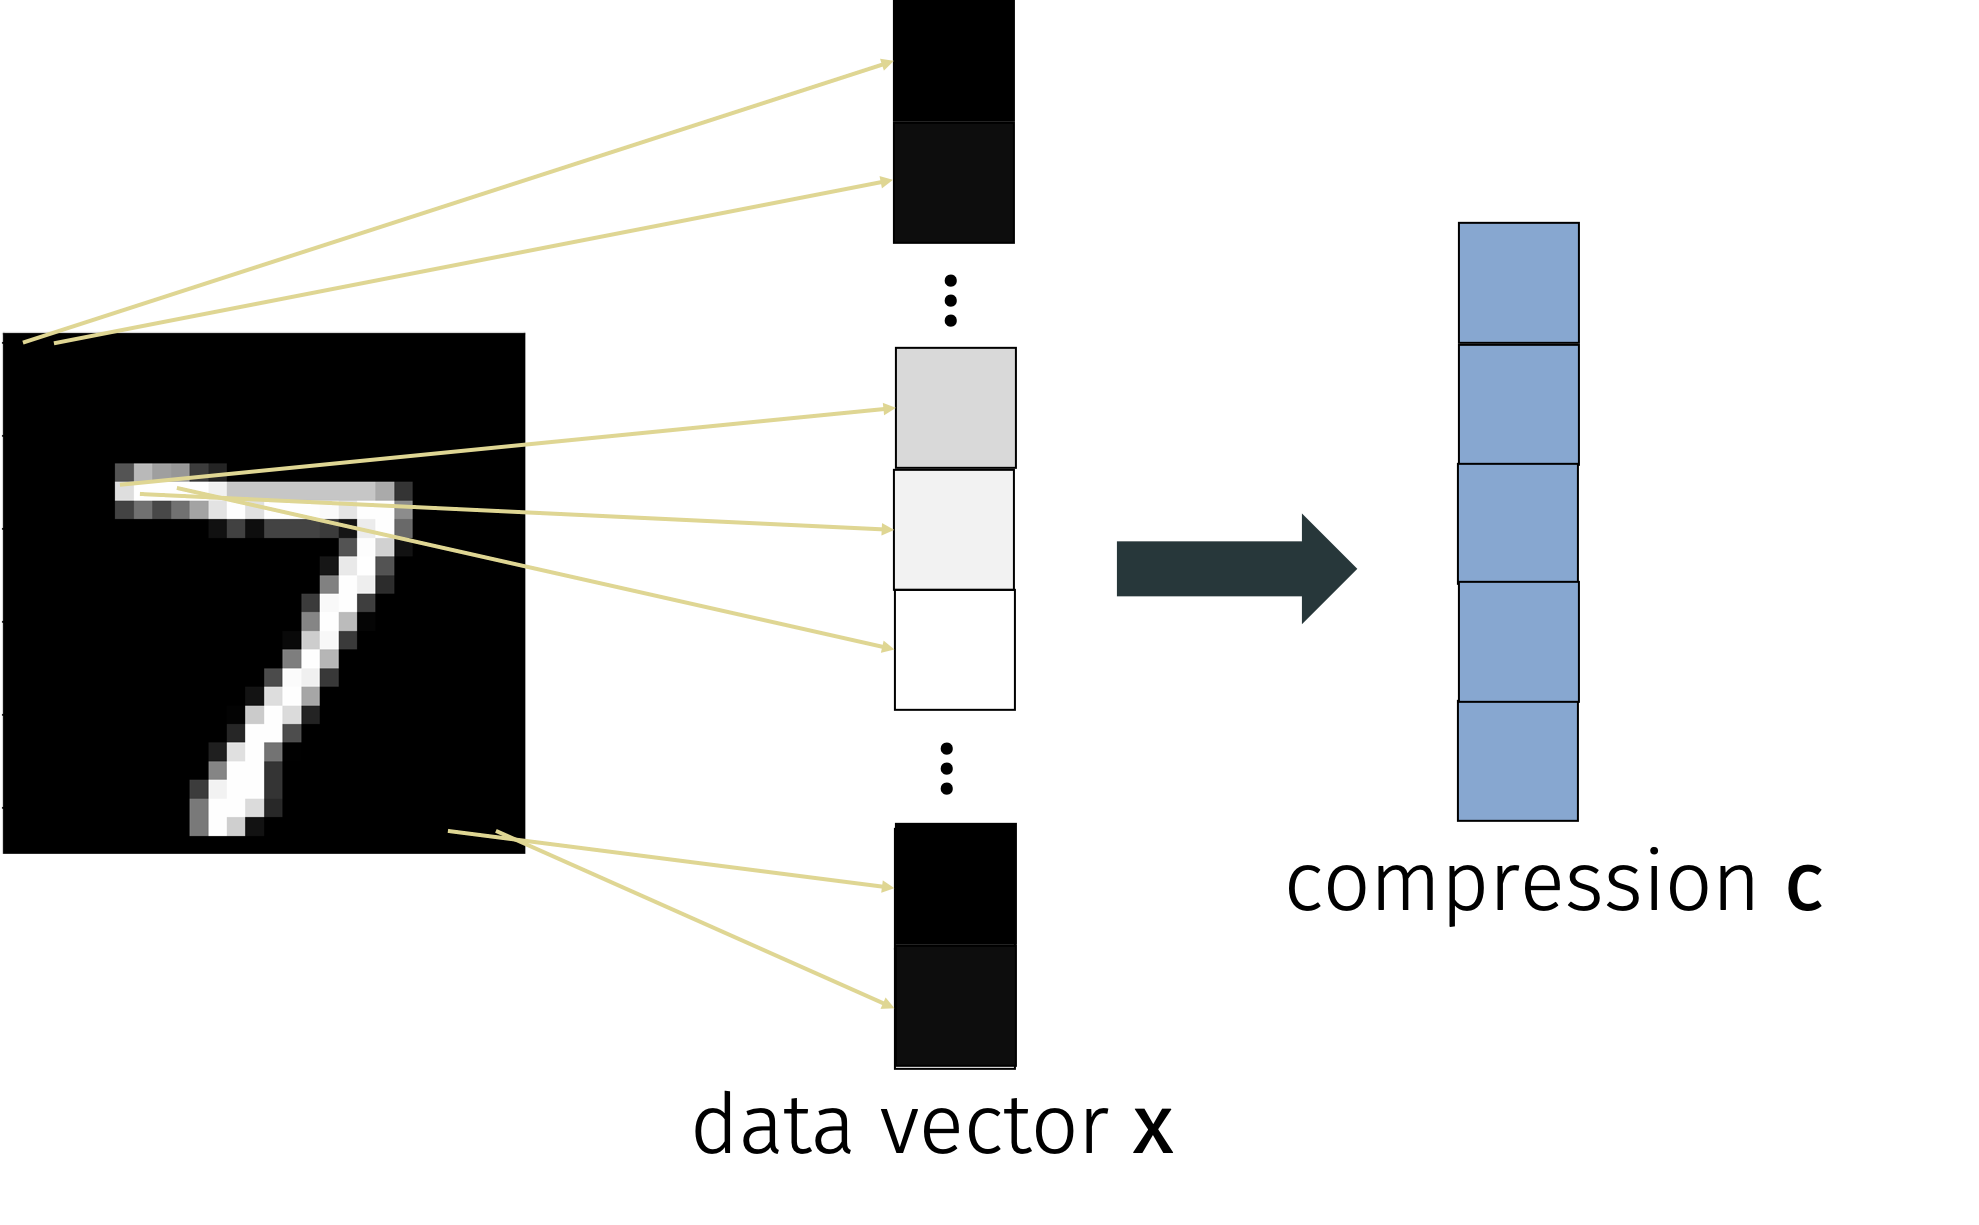
\includegraphics[width=.6\textwidth]{vectorize.png}
%	\end{center}
%\end{frame}

%\begin{frame}
%	\frametitle{spectral methods}
%	\textbf{Main difference from randomized methods:}
%	\begin{center}
%			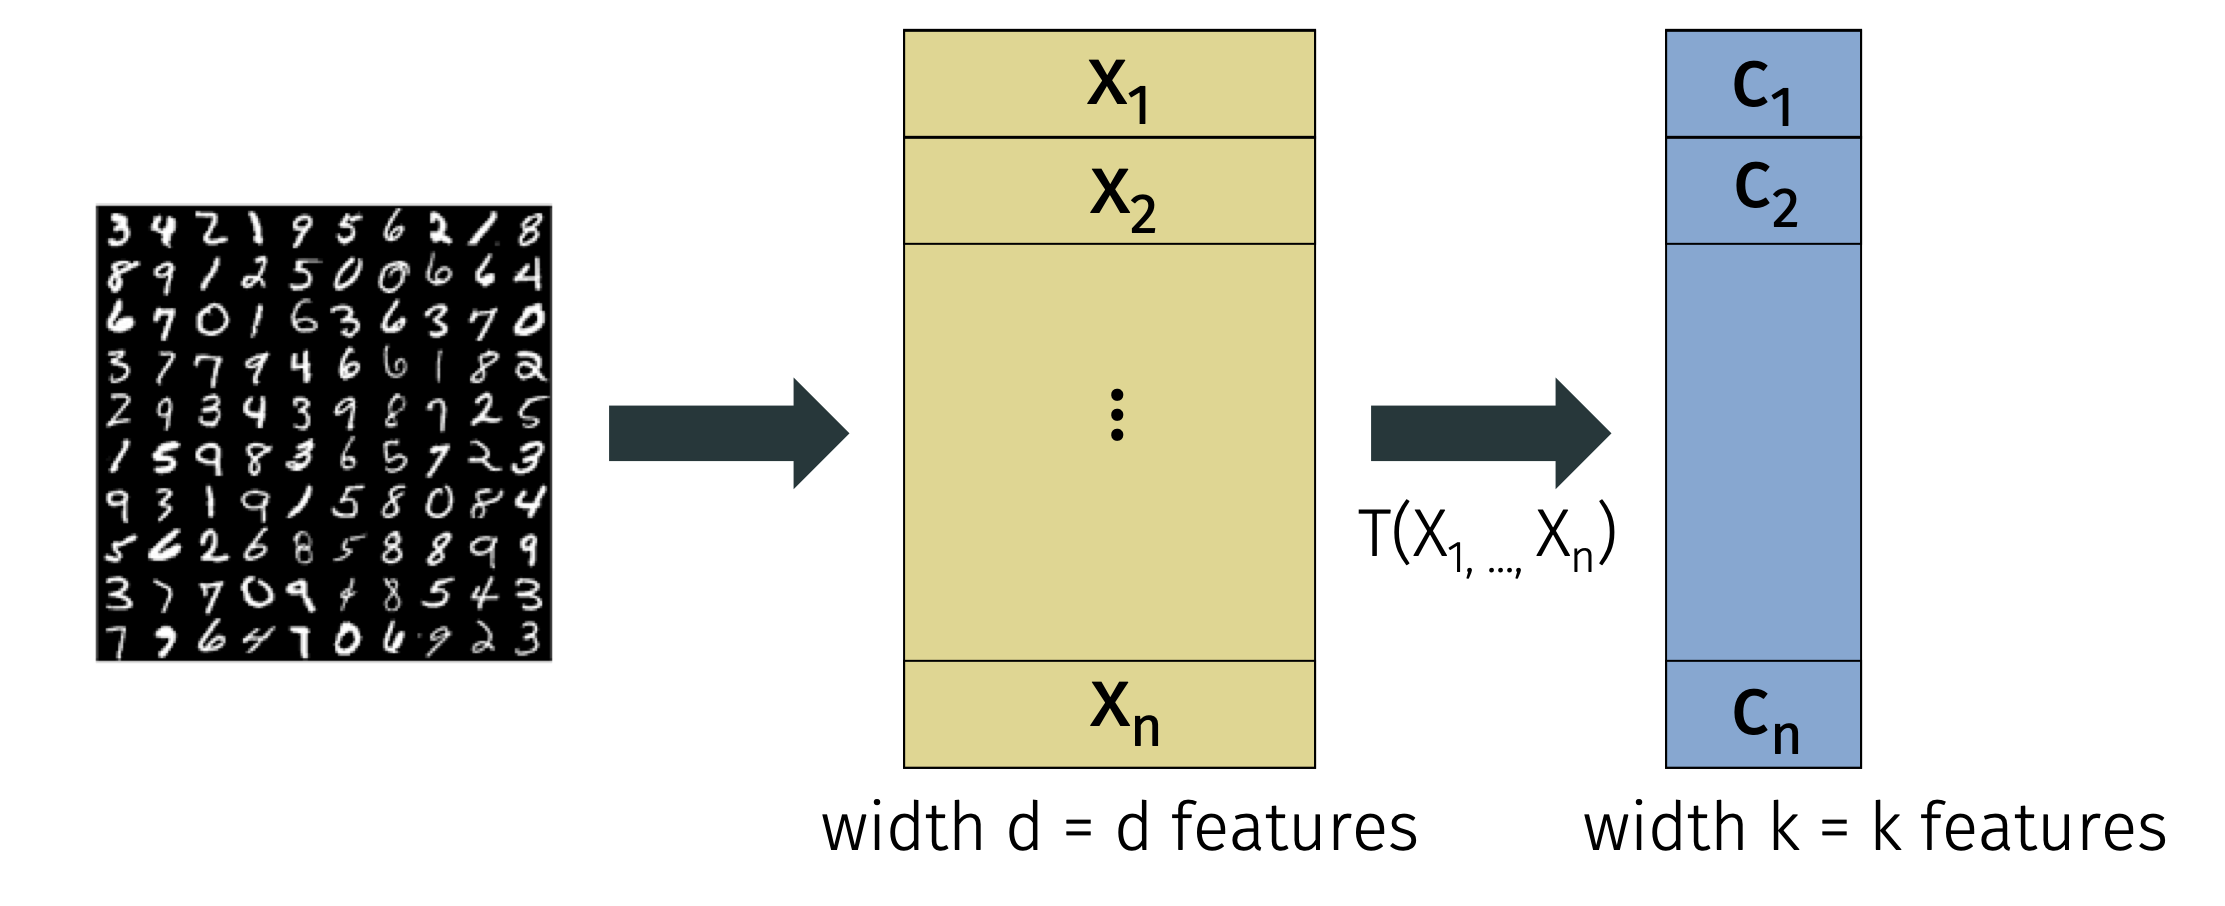
\includegraphics[width=.8\textwidth]{learned_compressioon.png}
%	\end{center}
%In this section, we will discuss \emph{data dependent} transformations. Johnson-Lindenstrauss, MinHash, SimHash were all \emph{data oblivious}. 
%\end{frame}
%
%\begin{frame}[t]
%	\frametitle{spectral methods}
%		\textbf{Advantages of data \alert{independent} methods:}
%	\vspace{8em}
%	
%	\textbf{Advantages of data \alert{dependent} methods:}
%\end{frame}

\begin{frame}[t]
	\frametitle{linear algebra reminder}
	If a \emph{square} matrix has orthonormal rows, it also has orthonormal columns:
	\begin{center}
		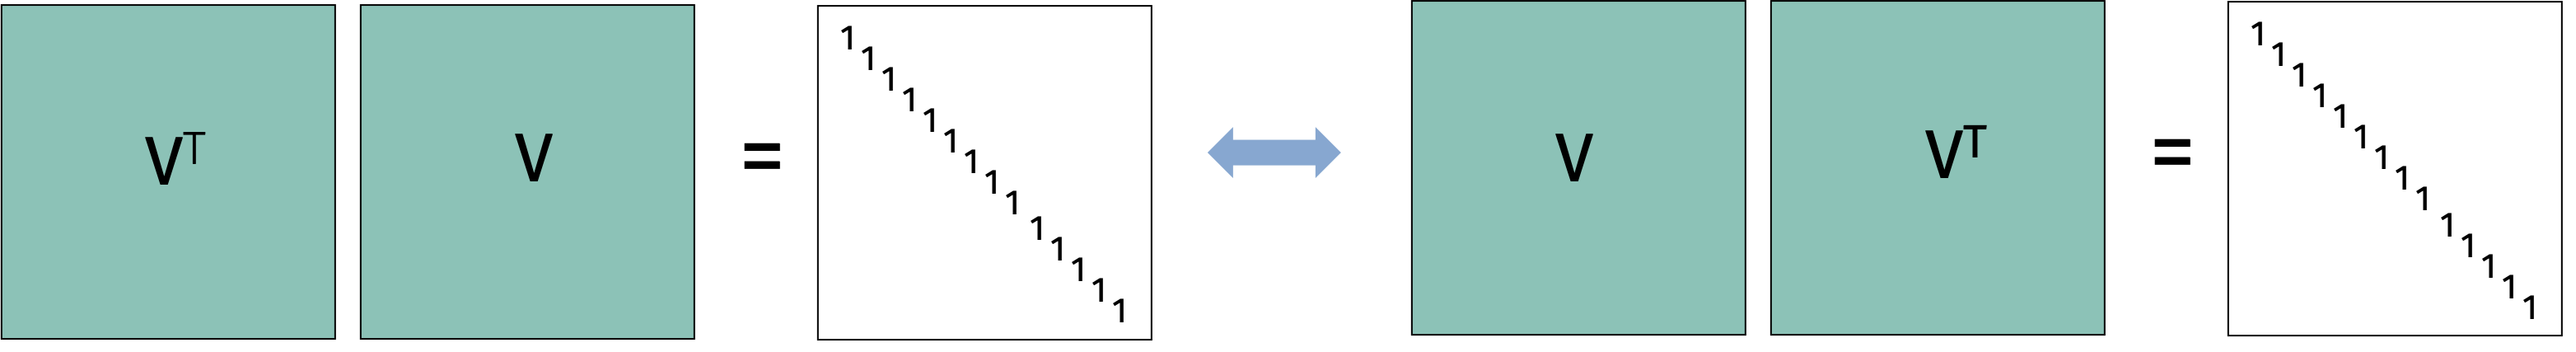
\includegraphics[width=\textwidth]{orth_square.png}
	\end{center}
	\begin{align*}
		\bv{V}^T\bv{V} = \bv{I} = \bv{V}\bv{V}^T
	\end{align*}
	
	\begin{align*}
		 \begin{bmatrix}
		 -0.62  &  0.78 &  -0.11\\
		-0.28   & -0.35 &  -0.89 \\
		-0.73  &  -0.52  &  0.44
		\end{bmatrix}
	\cdot 
		\begin{bmatrix}
   -0.62 &   -0.28 &   -0.73\\
0.78 &   -0.35  & -0.52\\
-0.11 &  -0.89 &    0.44
	\end{bmatrix}
= 		 \begin{bmatrix}
	1 &  0 &  0\\
	0   & 1 &  0 \\
	0  &  0  &  1
\end{bmatrix}
	\end{align*}
\end{frame}

\begin{frame}[t]
	\frametitle{linear algebra reminder}
	Implies that for any vector $\bv{x}$, $\|\bv{V}\bv{x}\|_2^2 = \|\bv{x}\|_2^2$ and $\|\bv{V}^T \bv{x}\|_2^2$.
	
	\vspace{1em}
	
	Same thing goes for Frobenius norm: for any matrix $\bv{X}$, $\|\bv{V}\bv{X}\|_F^2 = \|\bv{X}\|_F^2$ and $\|\bv{V}^T \bv{X}\|_F^2 = \|\bv{X}\|_F^2$.
\end{frame}

\begin{frame}[t]
	\frametitle{linear algebra reminder}
	The same is \emph{not true} for rectangular matrices:
	\begin{center}
		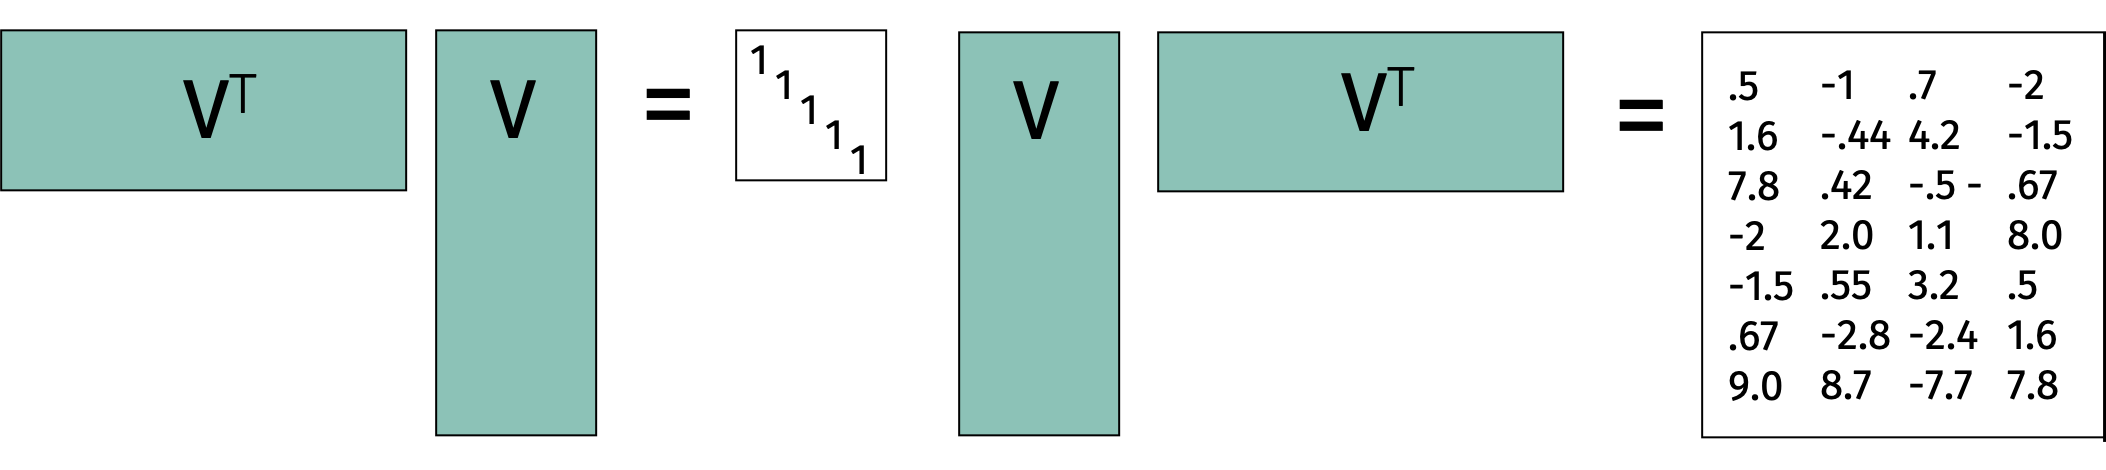
\includegraphics[width=\textwidth]{orth_rect.png}
	\end{center}
	\begin{align*}
		\bv{V}^T\bv{V} &= \bv{I} & &\text{but} & \bv{V}\bv{V}^T & \neq \bv{I}
	\end{align*}

For any $\bv{x}$, $\|\bv{V}\bv{x}\|_2^2 =\|\bv{x}\|_2^2$ \emph{but} $\|\bv{V}^T\bv{x}\|_2^2 \neq \|\bv{x}\|_2^2$ in general.  


%Equivalently, $\bv{x}$, $\|\bv{x}^T\bv{V}^T\|_2^2 =\|\bv{x}\|_2^2$ \emph{but} $\|\bv{x}^T\bv{V}\|_2^2 \neq \|\bv{x}\|_2^2$ in general.  
	
\end{frame}

\begin{frame}[t]
	\frametitle{linear algebra reminder}
	Multiplying a vector by $\bv{V}$ with orthonormal columns \emph{rotates and/or reflects} the vector. 
	\begin{center}
		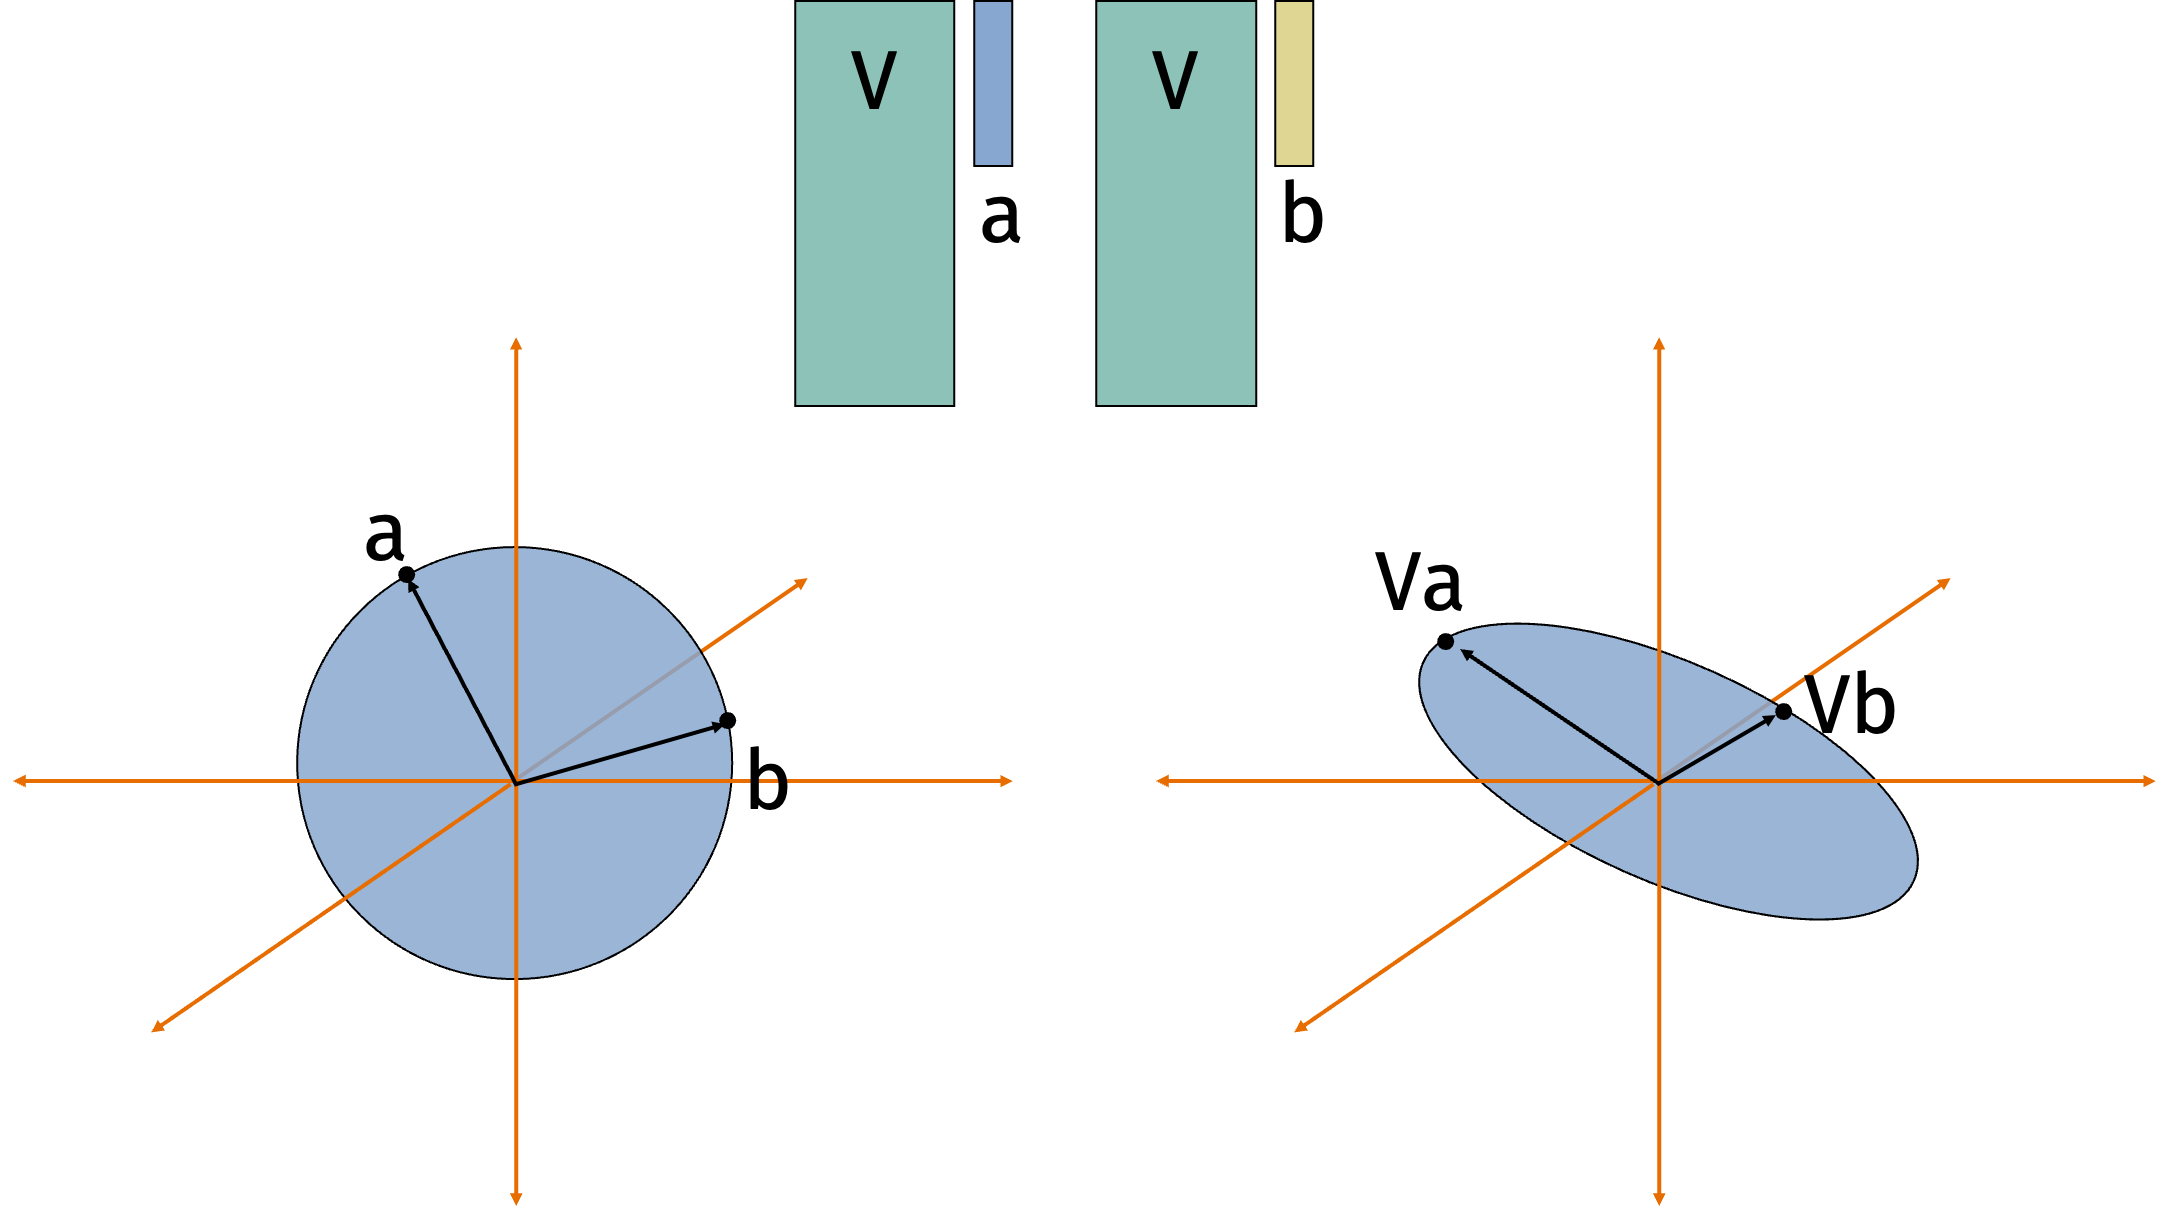
\includegraphics[width=\textwidth]{rotation_new.png}
	\end{center}
\end{frame}

\begin{frame}[t]
	\frametitle{linear algebra reminder}
	Multiplying a vector by a rectangular matrix $\bv{V}^T$ with orthonormal rows \emph{projects} the vector (representing it as coordinates in the lower dimensional space). 
	\begin{center}
		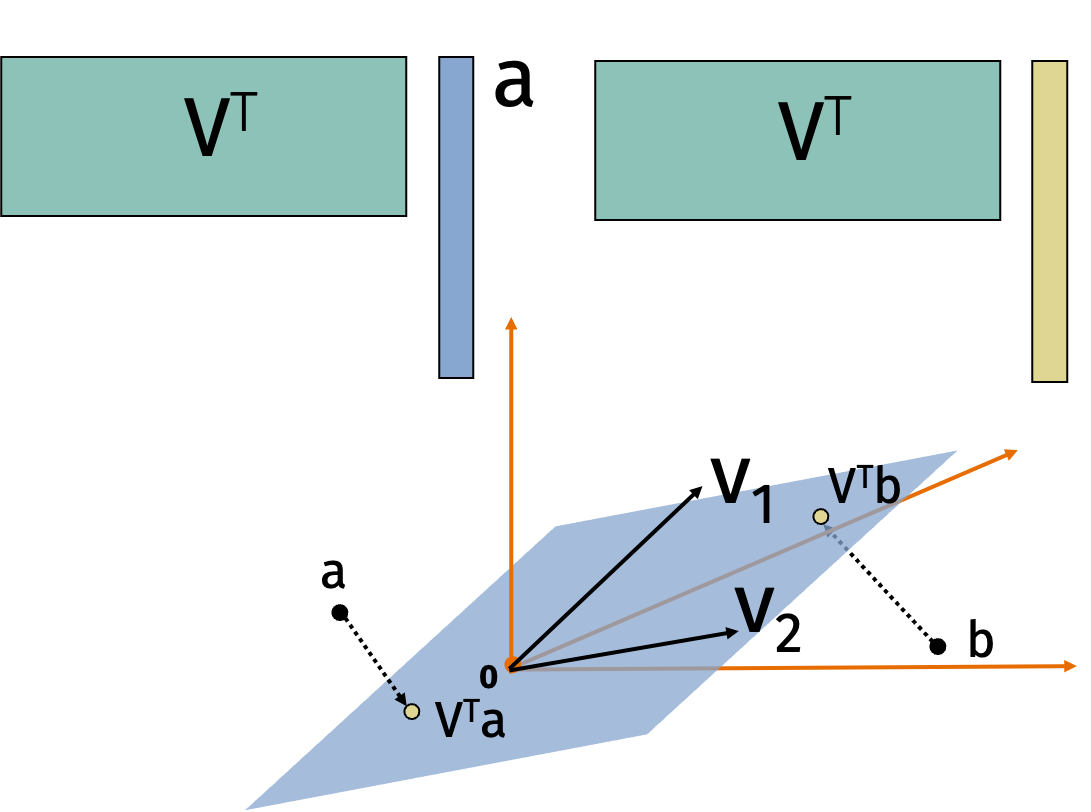
\includegraphics[width=.6\textwidth]{project.png}
	\end{center}
So we always have that $\|\bv{V}^T\bv{x}\|_2 \leq \|\bv{x}\|_2$.
\end{frame}

\begin{frame}
	\frametitle{singular value decomposition}
	\begin{center}
		\alert{One of the most fundamental results in linear algebra.}
	\end{center}
\vspace{-.5em}
	\emph{Any} matrix $\bv{X}$ can be written:
	\begin{center}
		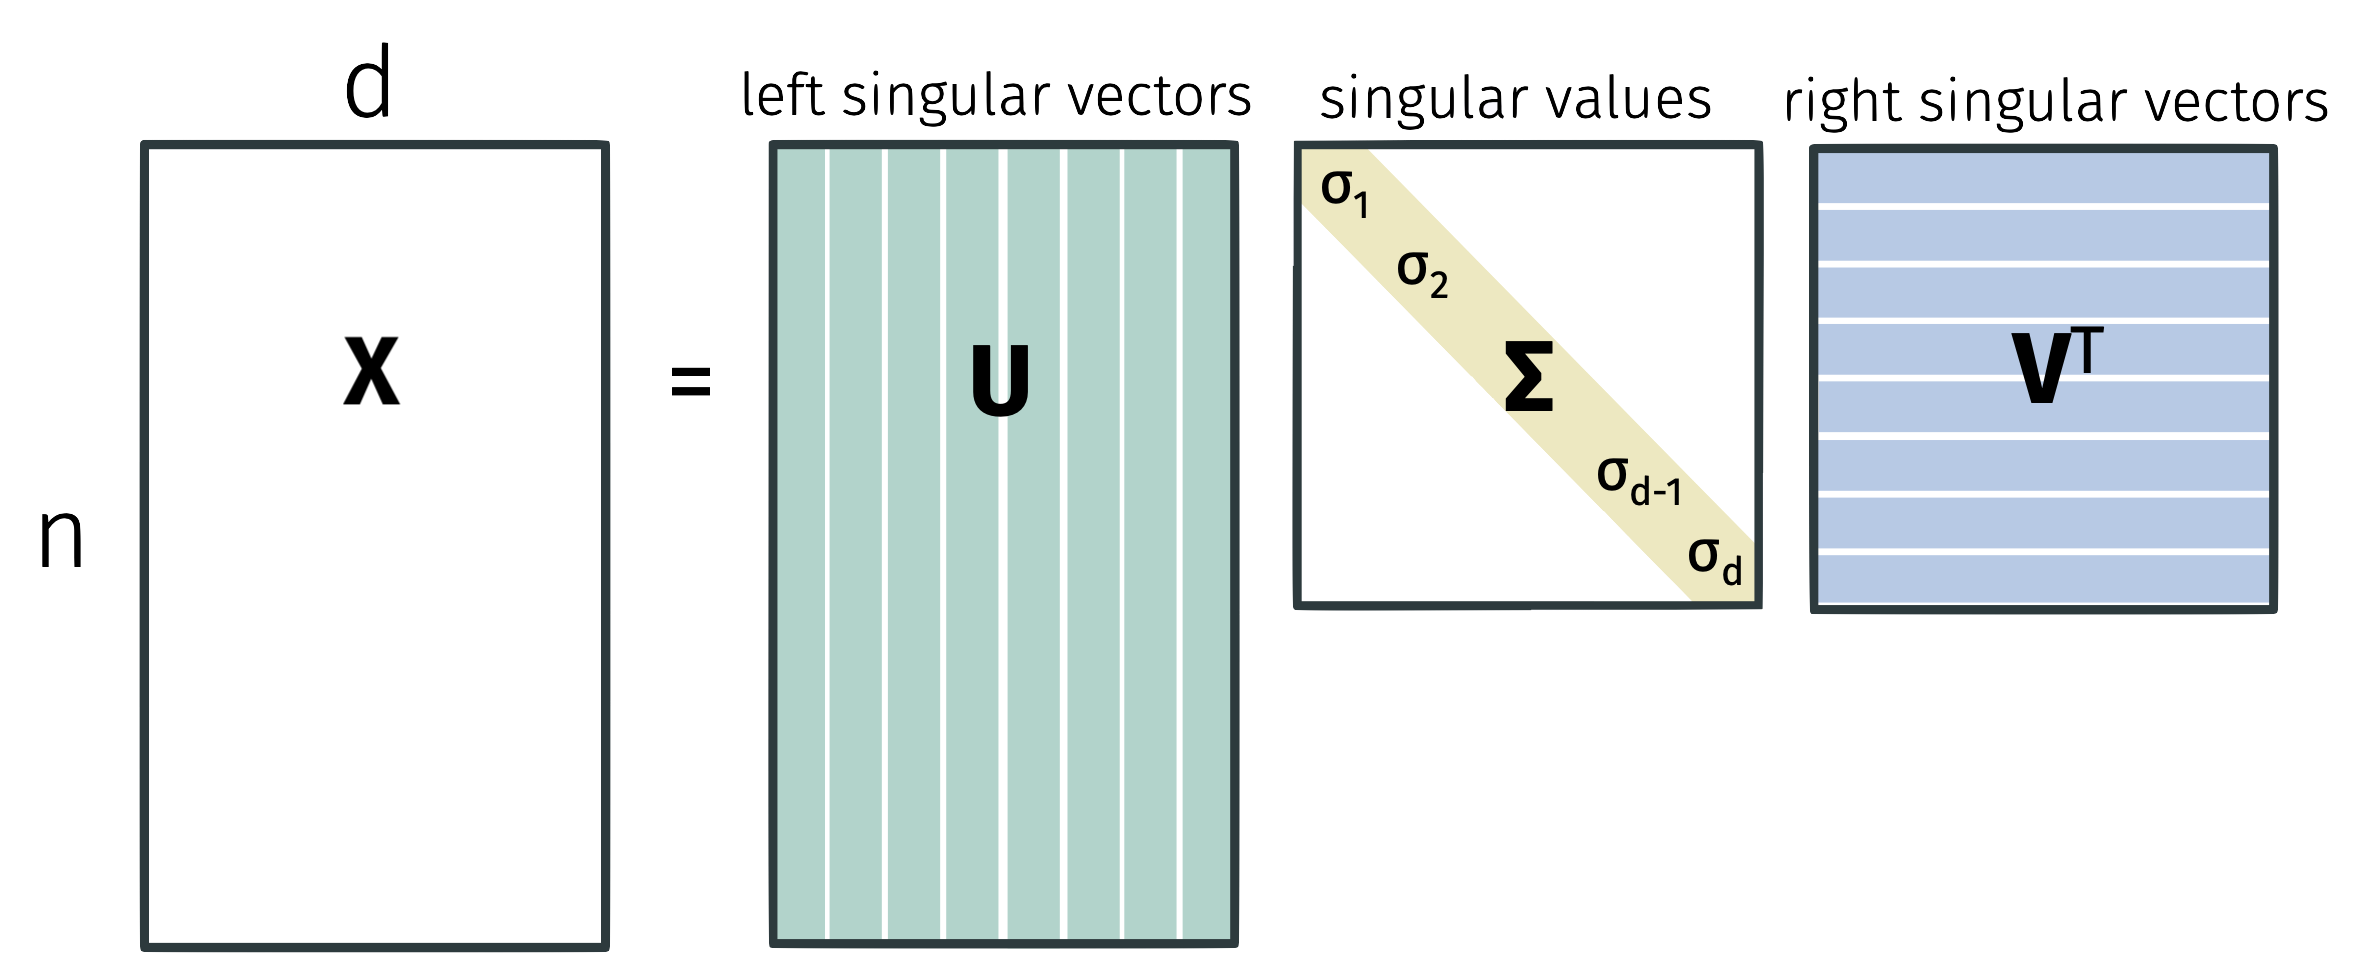
\includegraphics[width=.9\textwidth]{svd.png}
	\end{center} 
	Where $\bv{U}^T\bv{U} = \bv{I}$,  $\bv{V}^T\bv{V} = \bv{I}$, and $\sigma_1 \geq \sigma_2 \geq \ldots \sigma_d \geq 0$. 
	
%	Note that $\sum_{i=1}^d \sigma_i^2 = \|\bv{X}\|_F^2$. 

Singular values are unique. Factors are not. E.g. would still get a valid SVD by multiplying both $i^\text{th}$ column of $\bv{V}$ and $\bv{U}$ by $-1$.
\end{frame}

\begin{frame}[t]
	\frametitle{singular value decomposition}
	\begin{center}
		\alert{Important \emph{take away} from singular value decomposition.}
	\end{center}
	
	Multiplying any vector $\bv{a}$ by a matrix $\bv{X}$ to form $\bv{Xa}$ can be viewed as a composition of 3 operations:
	\begin{enumerate}
		\item Rotate/reflect the vector (multiplication by  to $\bv{V}^T$). 
		\item Scale the coordinates (multiplication by $\bs{\Sigma}$. 
		\item Rotate/reflect the vector again (multiplication by $\bv{U}$). 
	\end{enumerate}
\end{frame}

\begin{frame}[t]
	\frametitle{singular value decomposition: rotate/reflect}
	\begin{center}
		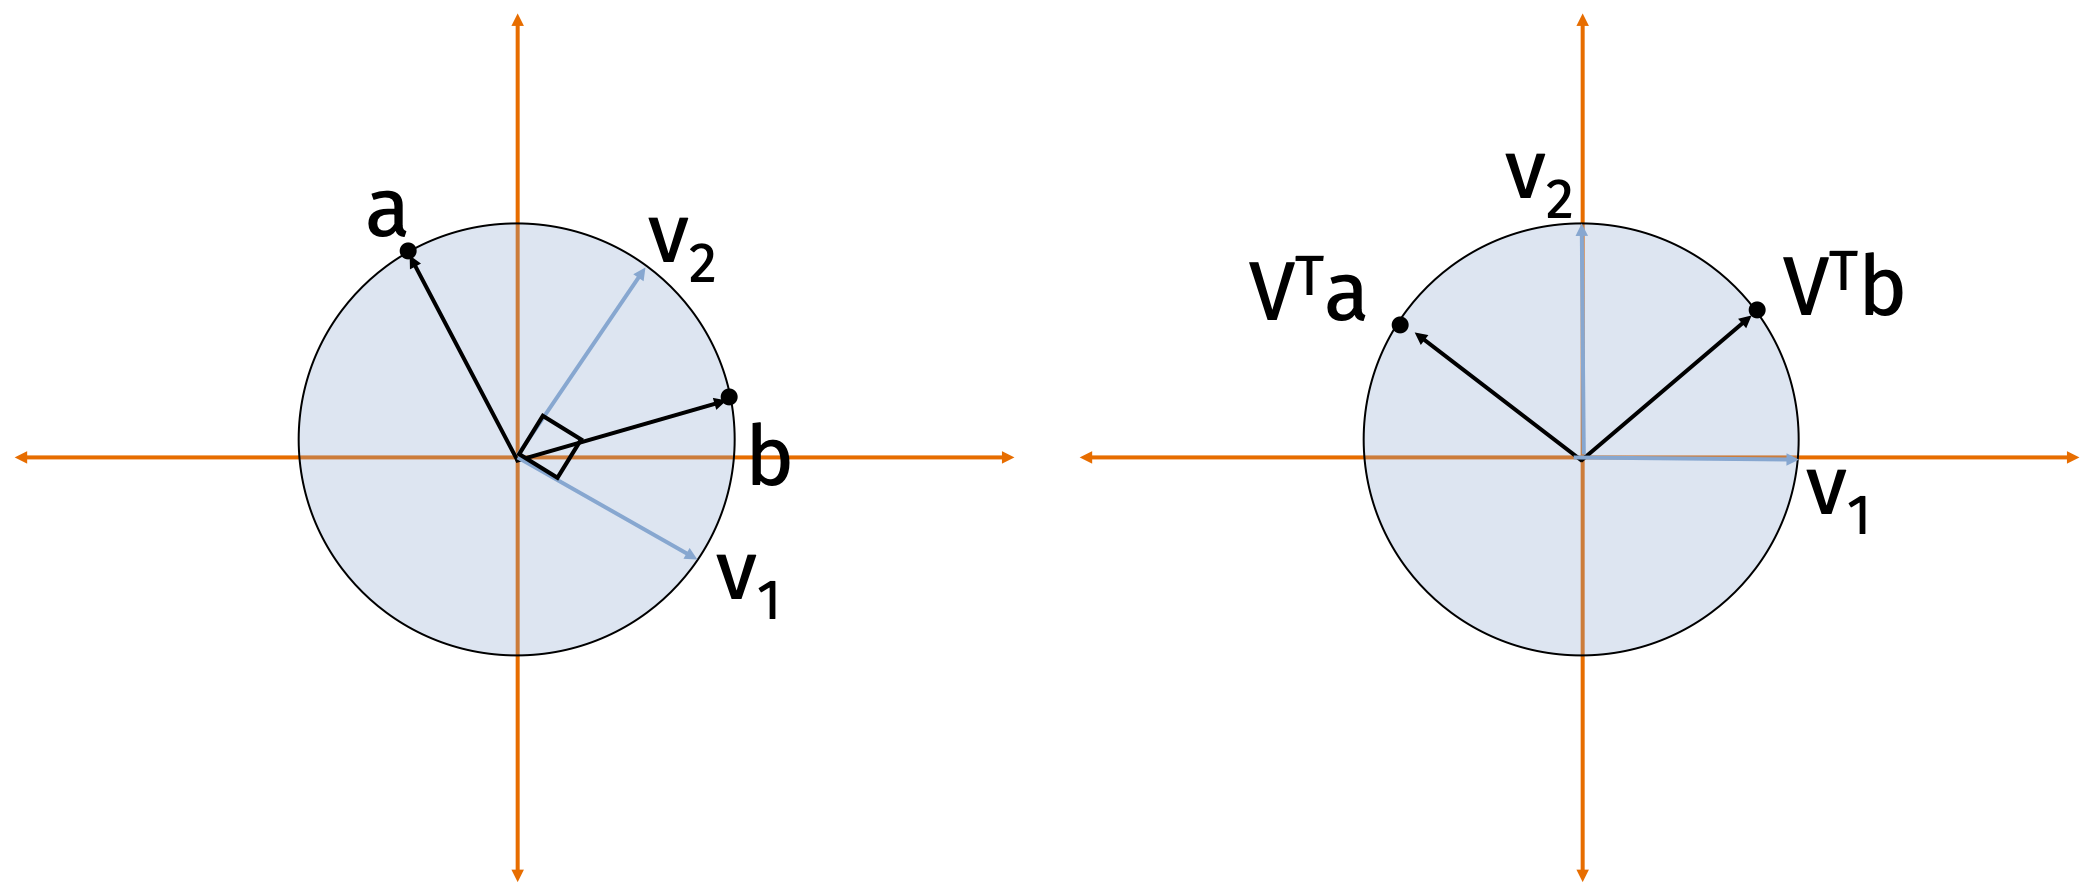
\includegraphics[width=.8\textwidth]{rotate1.png}
		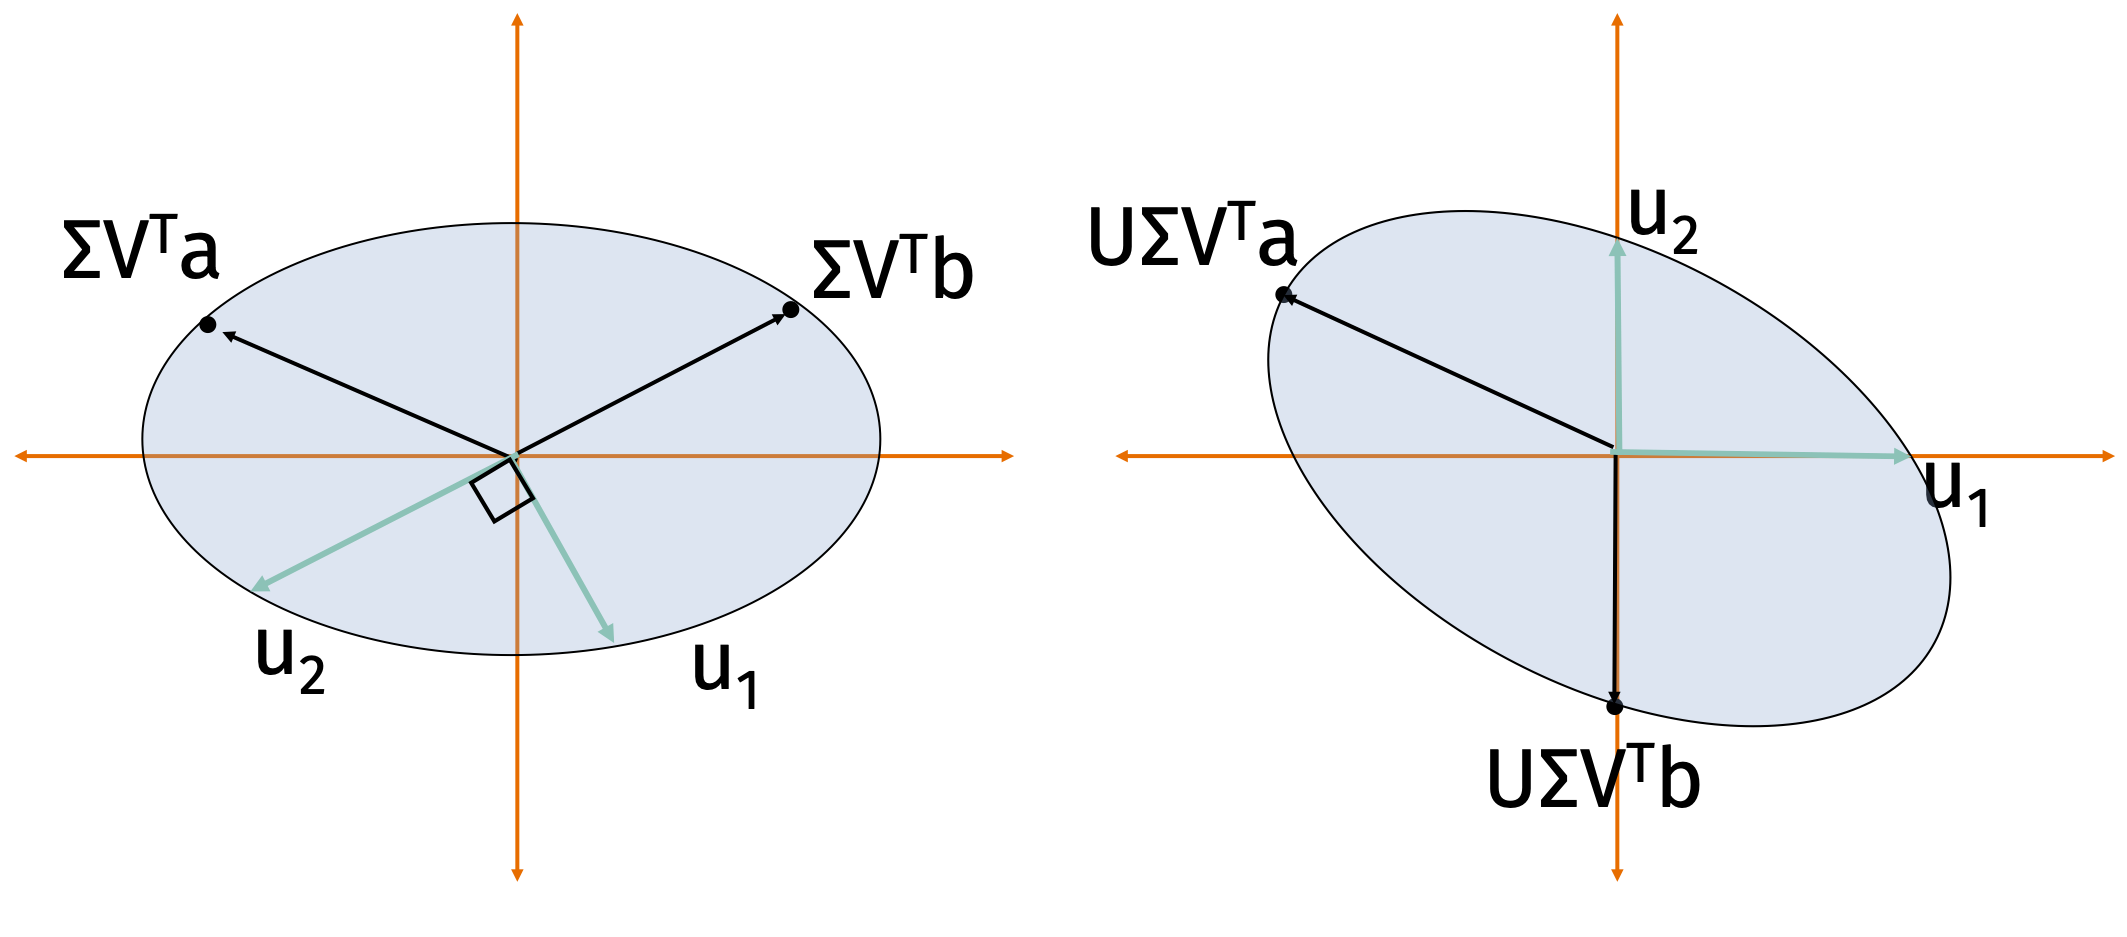
\includegraphics[width=.8\textwidth]{rotate2.png}
	\end{center}
\end{frame}

\begin{frame}[t]
	\frametitle{comparison to eigendecomposition}
	Recall that an eigenvalue of a \emph{square} matrix $\bv{X} \in \R^{d\times d}$ is any vector $\bv{v}$ such that $\bv{X}\bv{v} = \lambda \bv{v}$. A matrix has at most $d$ linearly independent eigenvectors. If a matrix has a full set of $d$ eigenvectors $\bv{v}_1, \ldots, \bv{v}_d$ with eigenvalues $\lambda_1, \ldots, \lambda_d$ it is called ``diagonalizable'' and can be written as:
	\begin{align*}
		\bv{V}\bs{\Lambda}\bv{V}^{-1}.
	\end{align*}
	$\bv{V}$'s columns are $\bv{v}_1, \ldots, \bv{v}_d$.
\end{frame}

\begin{frame}
		\frametitle{comparison to eigendecomposition}
		\begin{columns}
			\begin{column}{.5\textwidth}
				\begin{center}
					\textbf{Singluar value decomposition}
				\end{center}
			\begin{itemize}
				\item Exists for all matrices, square or rectangular.
				\item Singular values are always positive.
				\item Factors $\bv{U}$ and $\bv{V}$ are orthogonal.
			\end{itemize}
			\end{column}
			\begin{column}{.5\textwidth}
					\begin{center}
					\textbf{Eigendecomposition}
					\end{center}
		\begin{itemize}
			\item Exists for \emph{some} square matrices.
			\item Eigenvalues can be positive or negative.
			\item Factor $\bv{V}$ is orthogonal if and only if $\bv{X}$ is symmetric.
		\end{itemize}
				\end{column}
		\end{columns}
\end{frame}

\begin{frame}[t]
	\frametitle{connection to eigendecomposition}
	\begin{itemize}
		\item $\bv{U}$ contains the orthogonal eigenvectors of $\bv{X}\bv{X}^T$. 
		\item $\bv{V}$ contains the orthogonal eigenvectors of $\bv{X}^T\bv{X}$. 
		\item $\sigma_i^2 = \lambda_i(\bv{X}\bv{X}^T) = \lambda_i(\bv{X}^T\bv{X})$
	\end{itemize}
	
\end{frame}


\begin{frame}[t]
	\frametitle{svd applications}
	Lots of applications. 
	\begin{itemize}
		\item Compute pseudoinverse $\bv{V}\bs{\Sigma}^{-1} \bv{U}^T$. 
		\item Read off condition number of $\bv{X}$, $\sigma_1^2/\sigma_d^2$. 
		\item Compute matrix norms. E.g. $\|\bv{X}\|_2 = \sigma_1$, $\|\bv{X}\|_F = \sqrt{\sum_{i=1}^d \sigma_i^2}$.
		\item Compute matrix square root -- i.e. find a matrix $\bv{B}$ such that $\bv{B}\bv{B}^T = \bv{X}$.  Used e.g. in sampling from Gaussian with covariance $\bv{X}$.
		\item Principal component analysis.
	\end{itemize}
	\begin{center}
		\alert{\textbf{Killer app:} Read off optimal \emph{low-rank} approximations for $\bv{X}$.}
	\end{center}
\end{frame} 

\begin{frame}[t]
	\frametitle{rank}
	The column span of a matrix $\bv{X}\in \R^{n\times d}$ is the set of all vectors that can be written as $\bv{X}\bv{a}$ for some $\bv{a}$.

	The dimension of the column span, $D_c$, is the maximum number of linear independent vectors in that set. 

	The row span of a matrix $\bv{X}\in \R^{n\times d}$ is the set of all vectors that can be written as $\bv{b}^T\bv{X}$ for some $\bv{b}$.

	The dimension of the row span, $D_r$, is the maximum number of linear independent vectors in that set. 
\end{frame}

\begin{frame}[t]
	\frametitle{rank}
	For a matrix $\bv{X}\in \R^{n\times d}$ we have:
	\begin{align*}
		D_c &\leq d\\
		D_r &\leq n \\
		D_c &= D_r.
	\end{align*}
	We call the value of $D_c = D_r$ the \emph{rank} of $\bv{X}$.
\end{frame}

\begin{frame}
	\frametitle{low-rank approximation}
	Approximate $\bv{X}$ as the product of two rank $k$ matrices:
	\vspace{-1em}
	\begin{center}
		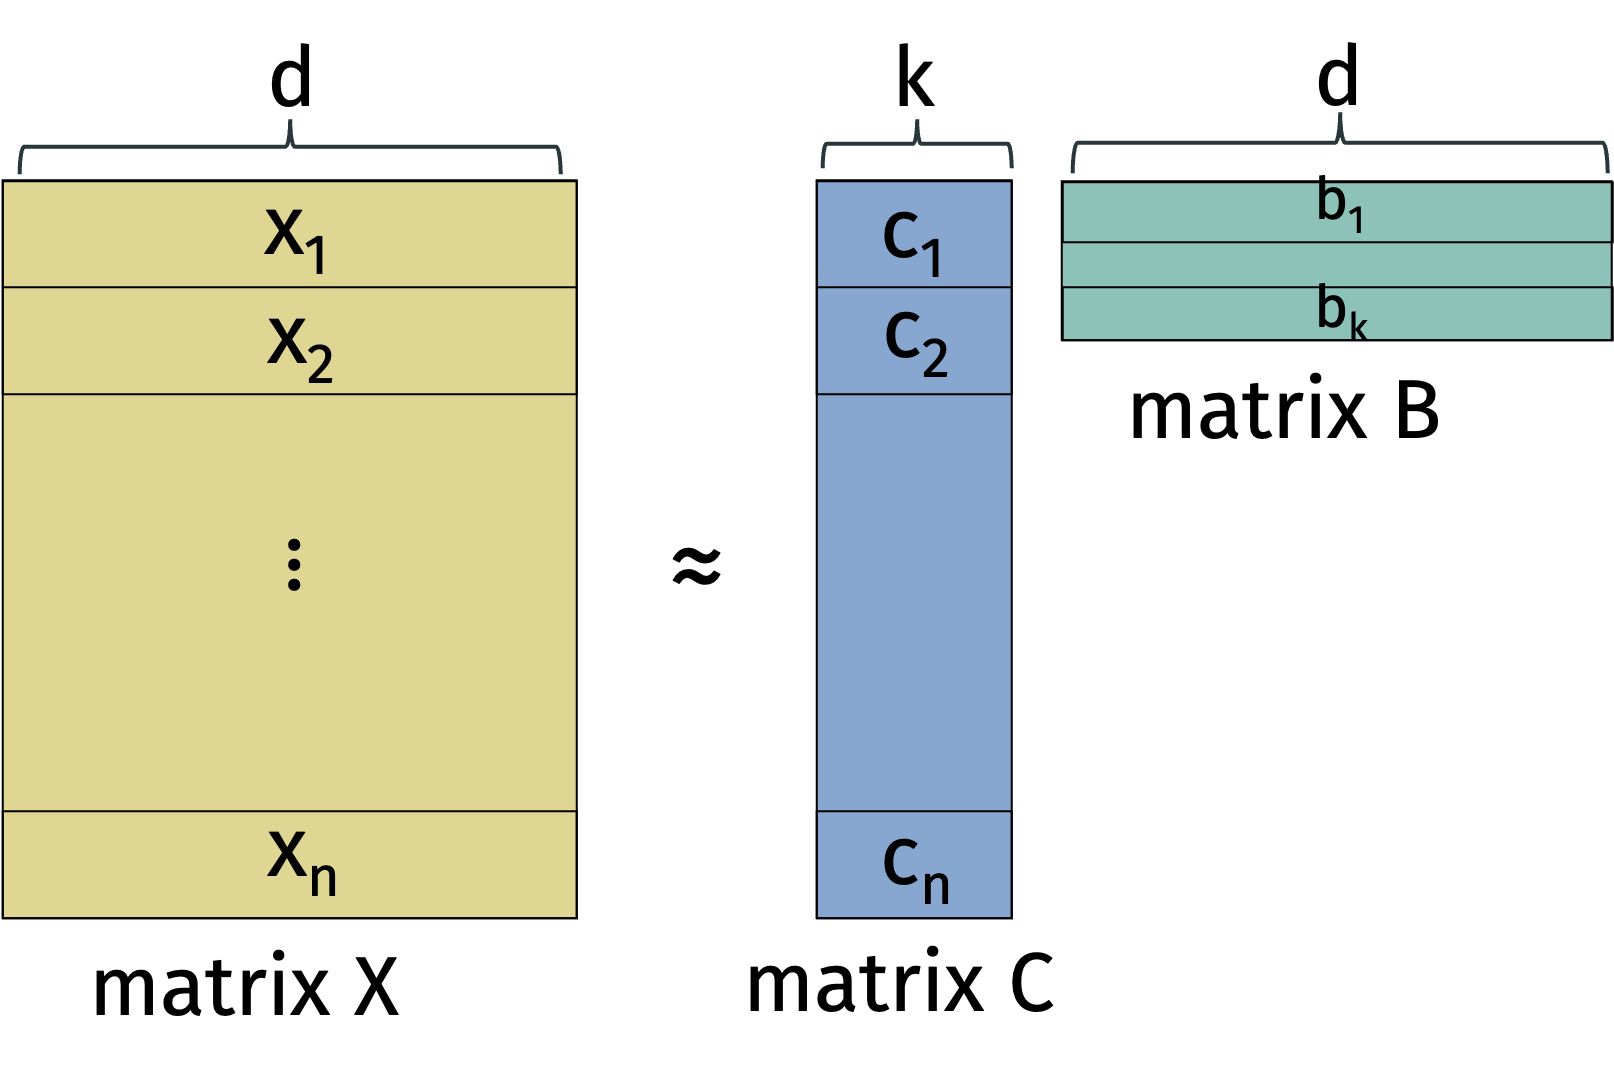
\includegraphics[width=.7\textwidth]{low-rank-basic.png}
	\end{center}
	\vspace{-.5em}
Typically choose $\bv{C}$ and $\bv{B}$ to minimize: 
\begin{align*}
	\min_{\bv{B},\bv{C}} \|\bv{X} - \bv{C}\bv{B}\|
\end{align*}
for some matrix norm. Common choice is $\|\bv{X} - \bv{C}\bv{B}\|_F^2$.
\end{frame}

\begin{frame}
	\frametitle{applications of low-rank approximation}
		\vspace{-1em}
	\begin{center}
		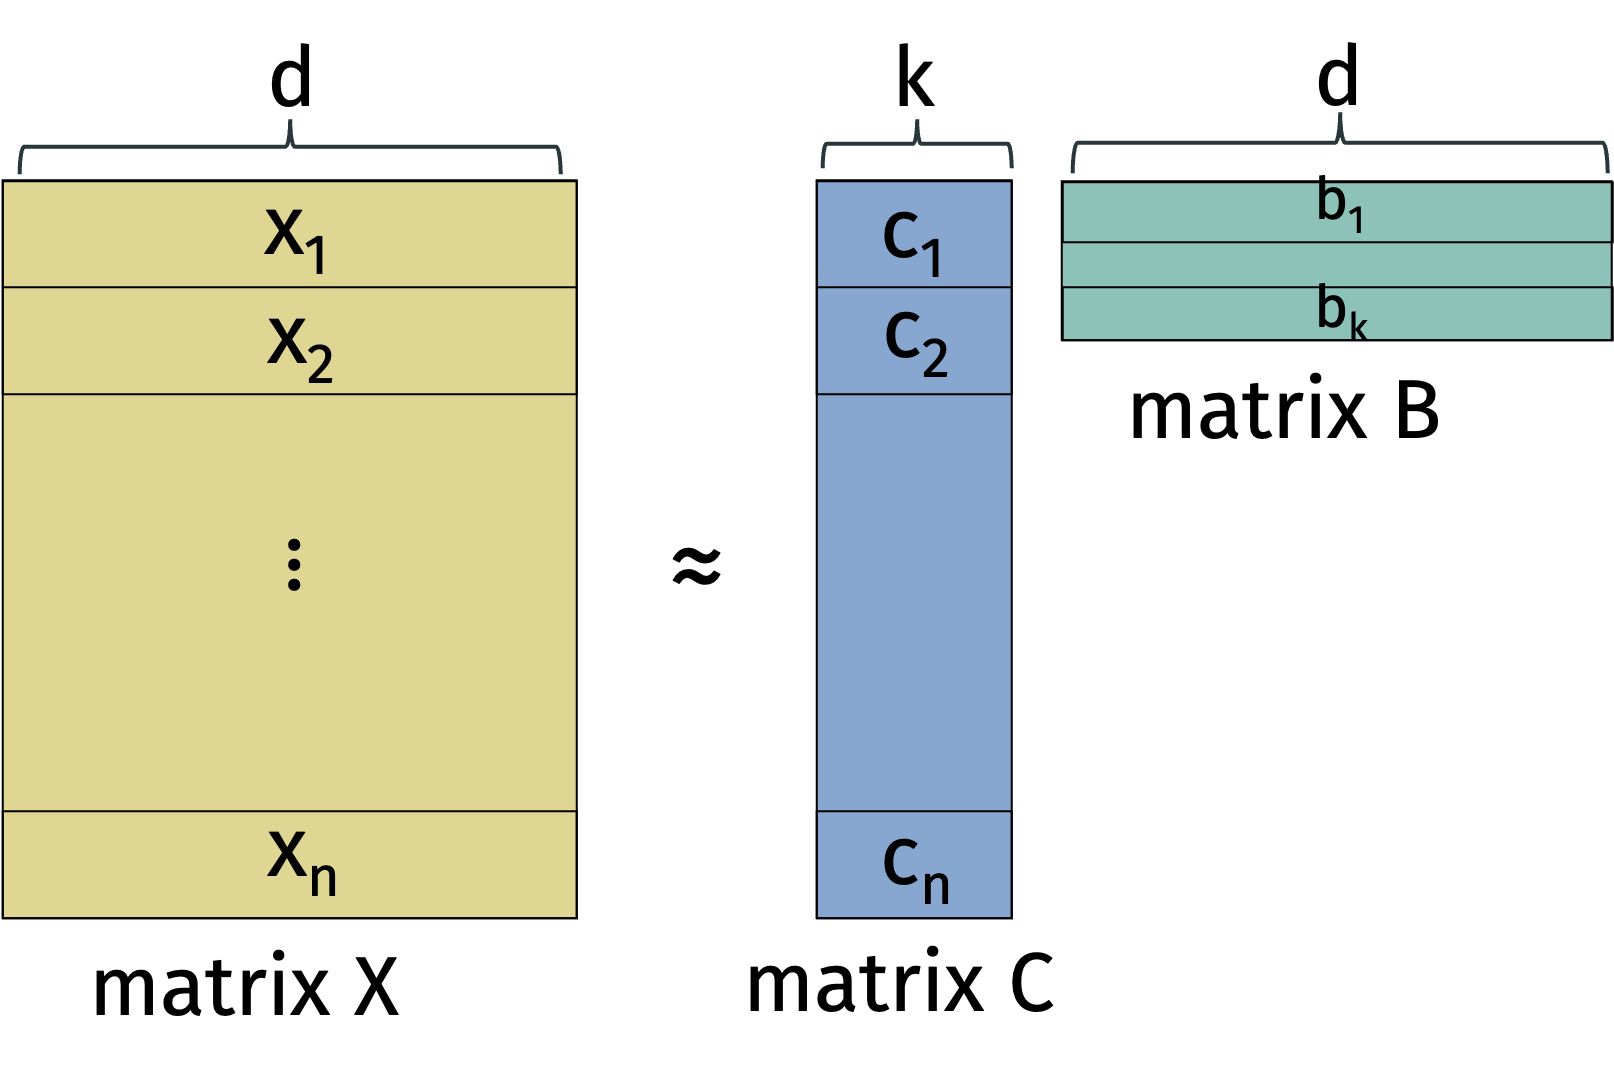
\includegraphics[width=.6\textwidth]{low-rank-basic.png}
	\end{center}
	\begin{itemize}
		\item $\bv{C} \bv{B}$ takes $O(k(n+d))$ space to store instead of $O(nd)$.
		\item Regression problems involving $\bv{C} \bv{B}$ can be solved in $O(nk^2)$ instead of $O(nd^2)$ time.
		\item Will see a bunch more in a minute.
	\end{itemize}
\end{frame}

\begin{frame}
	\frametitle{low-rank approximation}
	Without loss of generality can assume that the right matrix is orthogonal. I.e. $\bv{W}^T$ with $\bv{W}^T\bv{W} = \bv{I}$
	\vspace{-1em}
	\begin{center}
		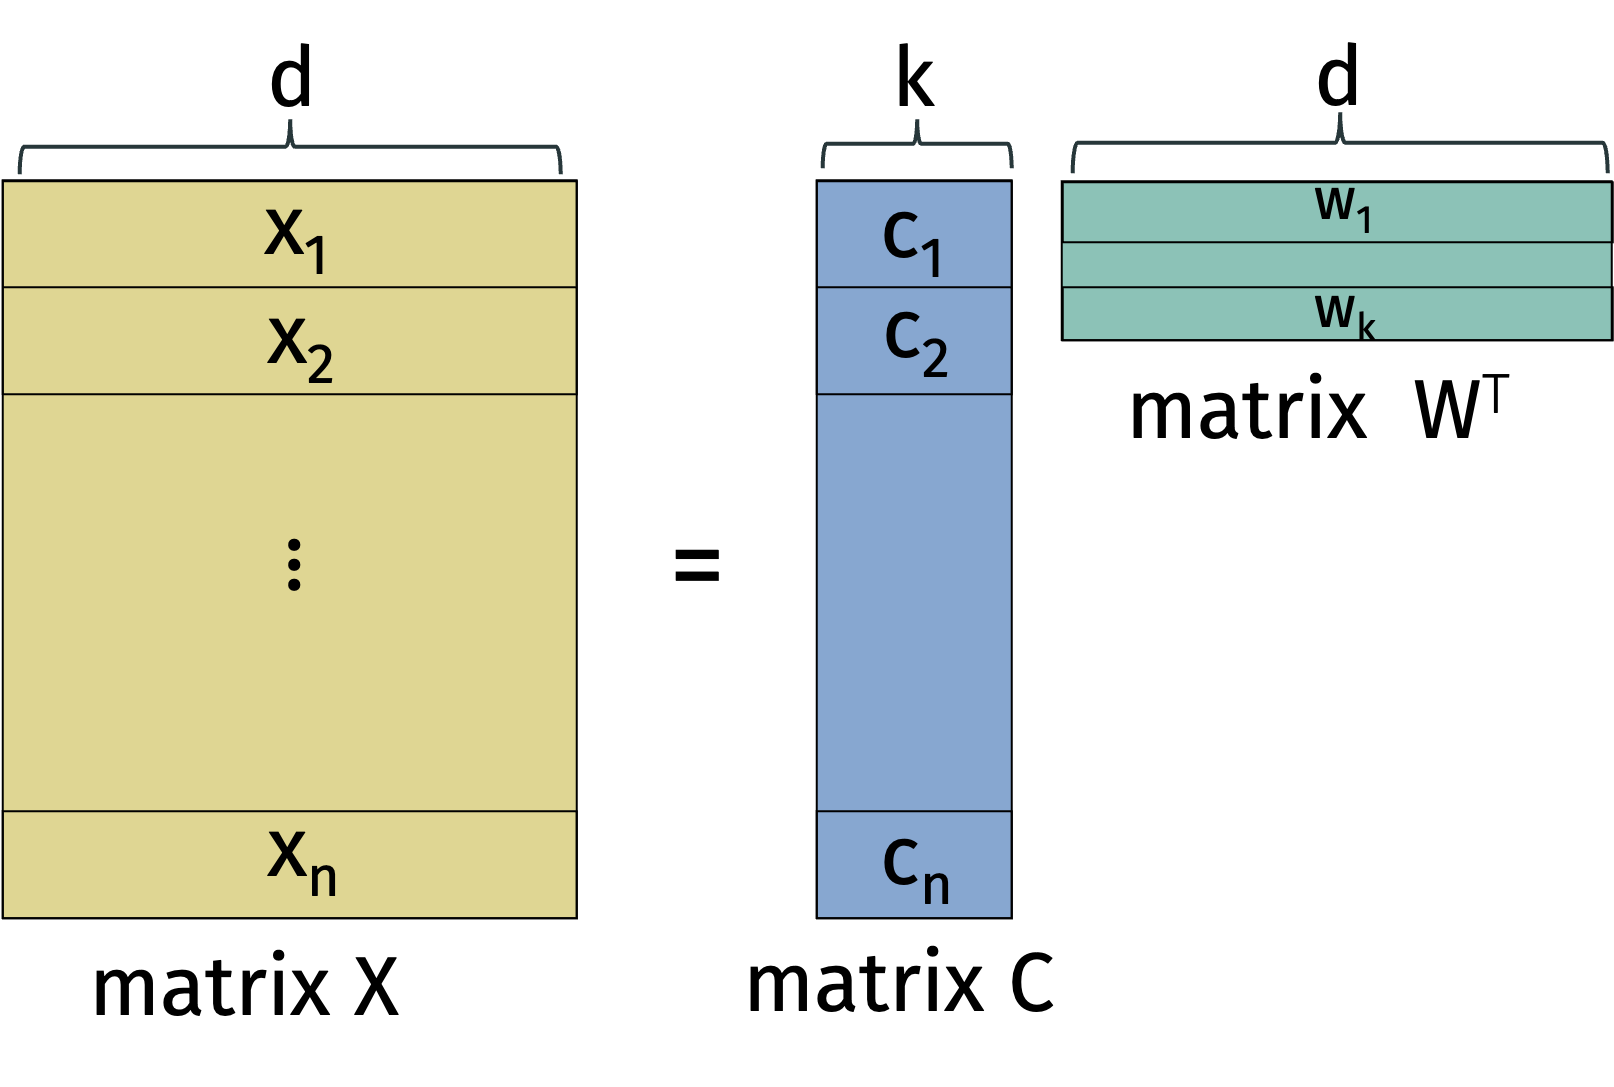
\includegraphics[width=.6\textwidth]{low-rank-orth.png}
	\end{center}
Then we should choose $\bv{C}$ to minimize:
\begin{align*}
	\min_{\bv{C}} \|\bv{X} - \bv{C}\bv{W}^T\|_F^2
\end{align*}
This is just $n$ least squares regression problems!
\end{frame}

\begin{frame}
	\frametitle{low-rank approximation}
	\begin{align*}
		\bv{c}_i = \argmin_{\bv{c}} \|\bv{W} \bv{c} - \bv{x}_i\|_2^2
	\end{align*}
\vspace{3em}

\begin{align*}
	\bv{c}_i  &= \bv{W}^T\bv{x}_i \\
	\bv{C} &= \bv{X}\bv{W}
\end{align*}

So our optimal low-rank approximation always has the form:
\begin{align*}
	\bv{X} \approx \bv{X}\bv{W}\bv{W}^T
\end{align*}
\end{frame}

\begin{frame}
	\frametitle{projection matrices}
	$\bv{W}\bv{W}^T$ is a symmetric \emph{projection matrix}.
	\begin{center}
		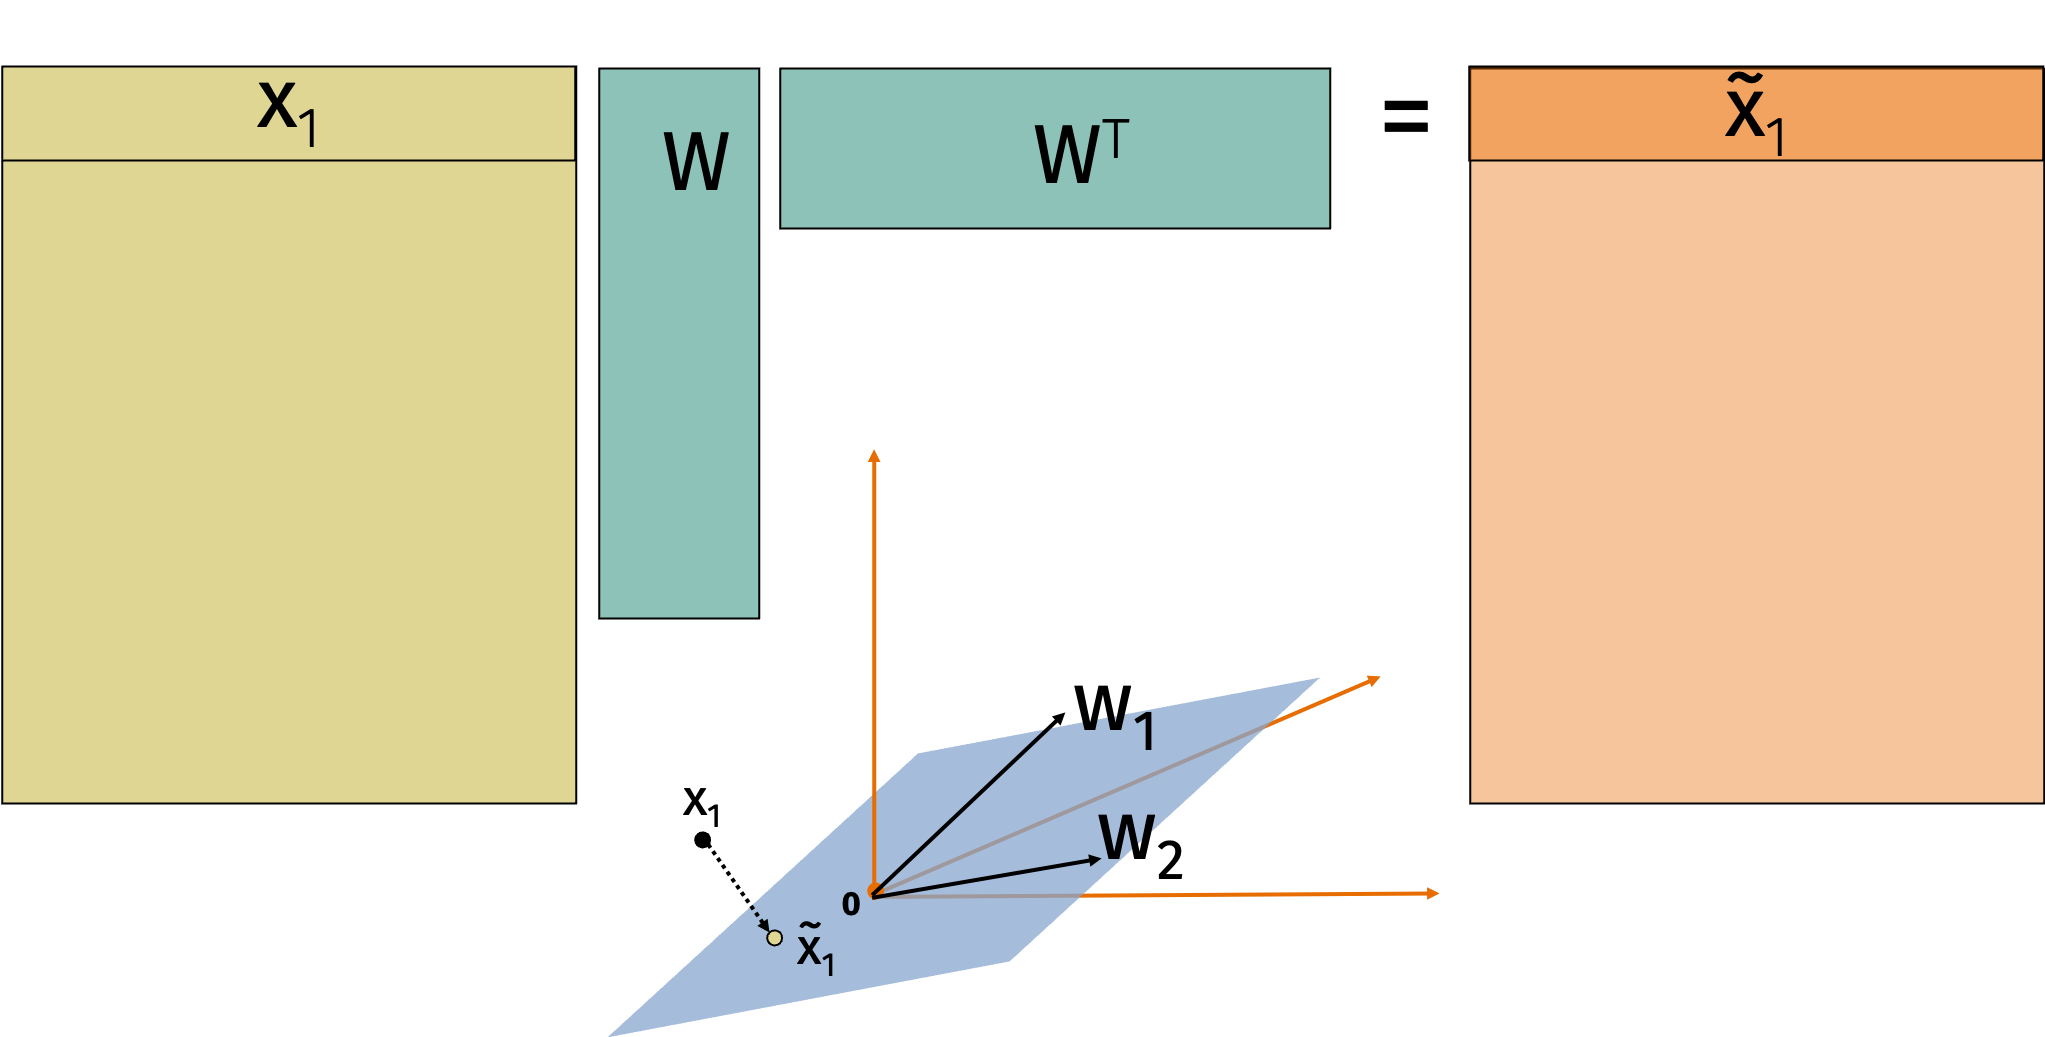
\includegraphics[width=\textwidth]{projection.png}
	\end{center}
%	When a data point $\bv{x}$ already lies in the subspace spanned by $\bv{V}$'s columns, projection doesn't do anything. So  $\bv{x} = \bv{x}\bv{V}\bv{V}^T$.
\end{frame}

\begin{frame}
	\frametitle{low-rank approximation}
	\vspace{-1em}
	\begin{center}
		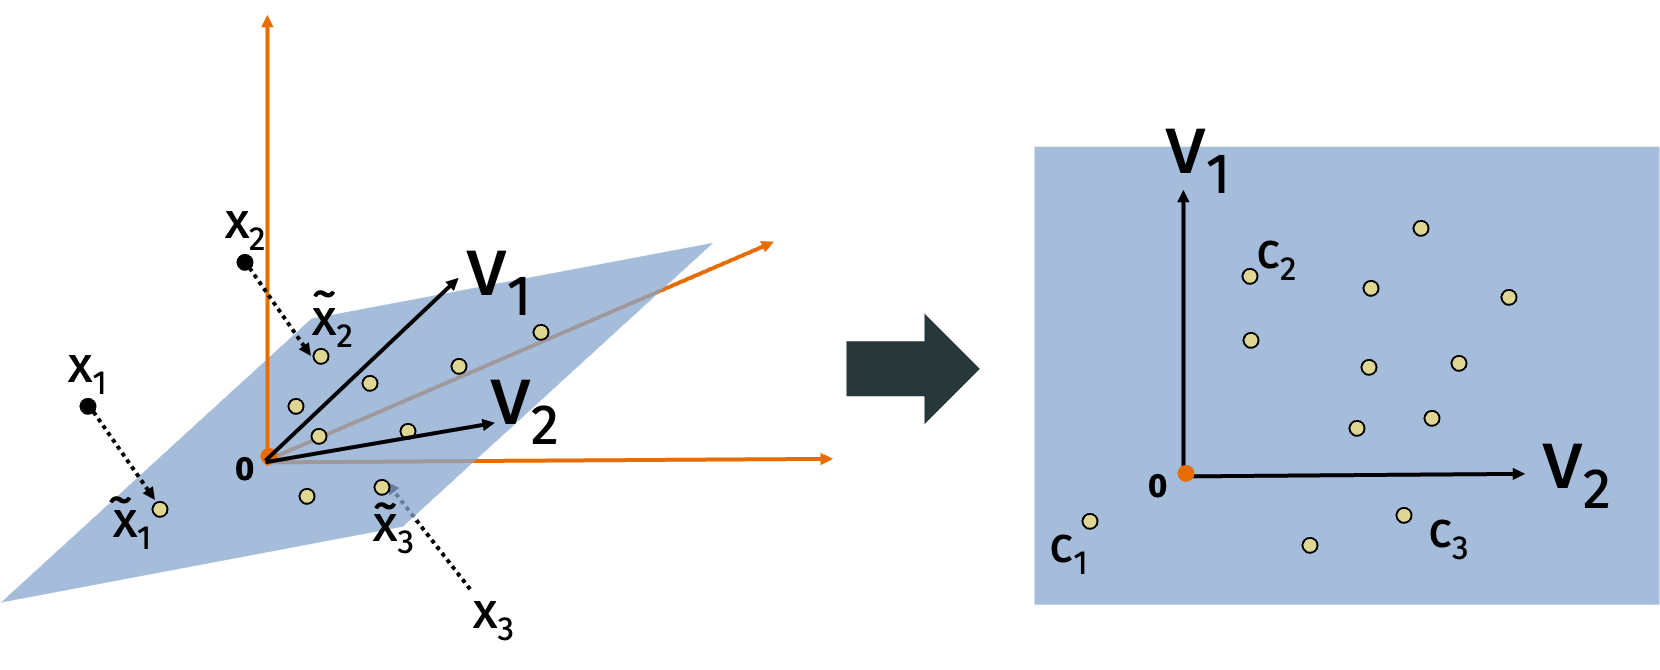
\includegraphics[width=.8\textwidth]{project_full.png}
	\end{center}
	\begin{center}
		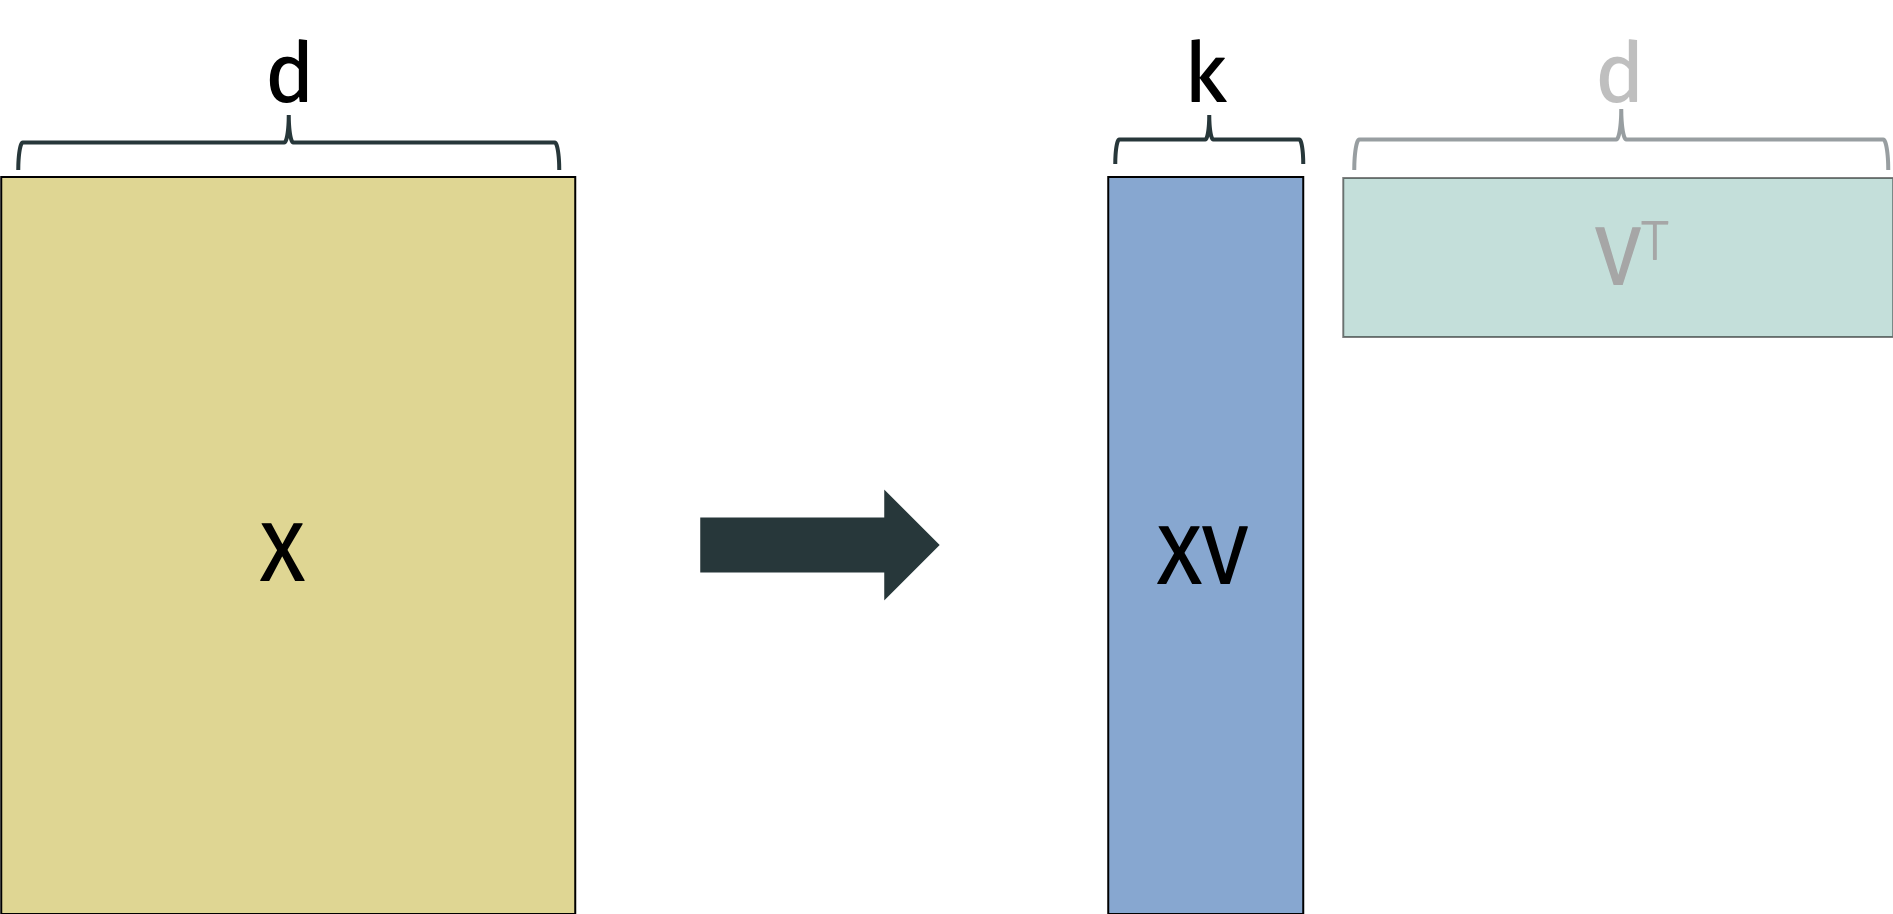
\includegraphics[width=.5\textwidth]{lowrankcompress.png}
	\end{center}
	$\bv{C} = \bv{XW}$ can be used as a compressed version of data matrix $\bv{X}$. 
\end{frame}

\begin{frame}
	\frametitle{data compression}
	Let $\bv{C} = \bv{XW}$. We have that:
	\begin{align*}
		\|\bv{x}_i - \bv{x}_j\|_2 \approx \|\bv{x}_i^T\bv{WW}^T- \bv{x}_j^T\bv{WW}^T\|_2 = \|\bv{c}_i - \bv{c}_i\|_2
	\end{align*}
Similarly, we expect that:
\begin{itemize}
	\item $\|\bv{x}_i\|_2 \approx \|\bv{c}_i\|_2$
	\item $\langle \bv{x}_i, \bv{x}_j \rangle \approx \langle \bv{c}_i, \bv{c}_j \rangle$
	\item etc.
\end{itemize}
\begin{center}
	\alert{How does this compare to Johnson-Lindenstrauss projection?}
\end{center}
\end{frame}

\begin{frame}
	\frametitle{why is data approximately low-rank?}
	Rows of $\bv{X}$ (data points) are approximately spanned by $k$ vectors. Columns of $\bv{X}$ (data features) are approximately spanned by $k$ vectors.
	\begin{center}
		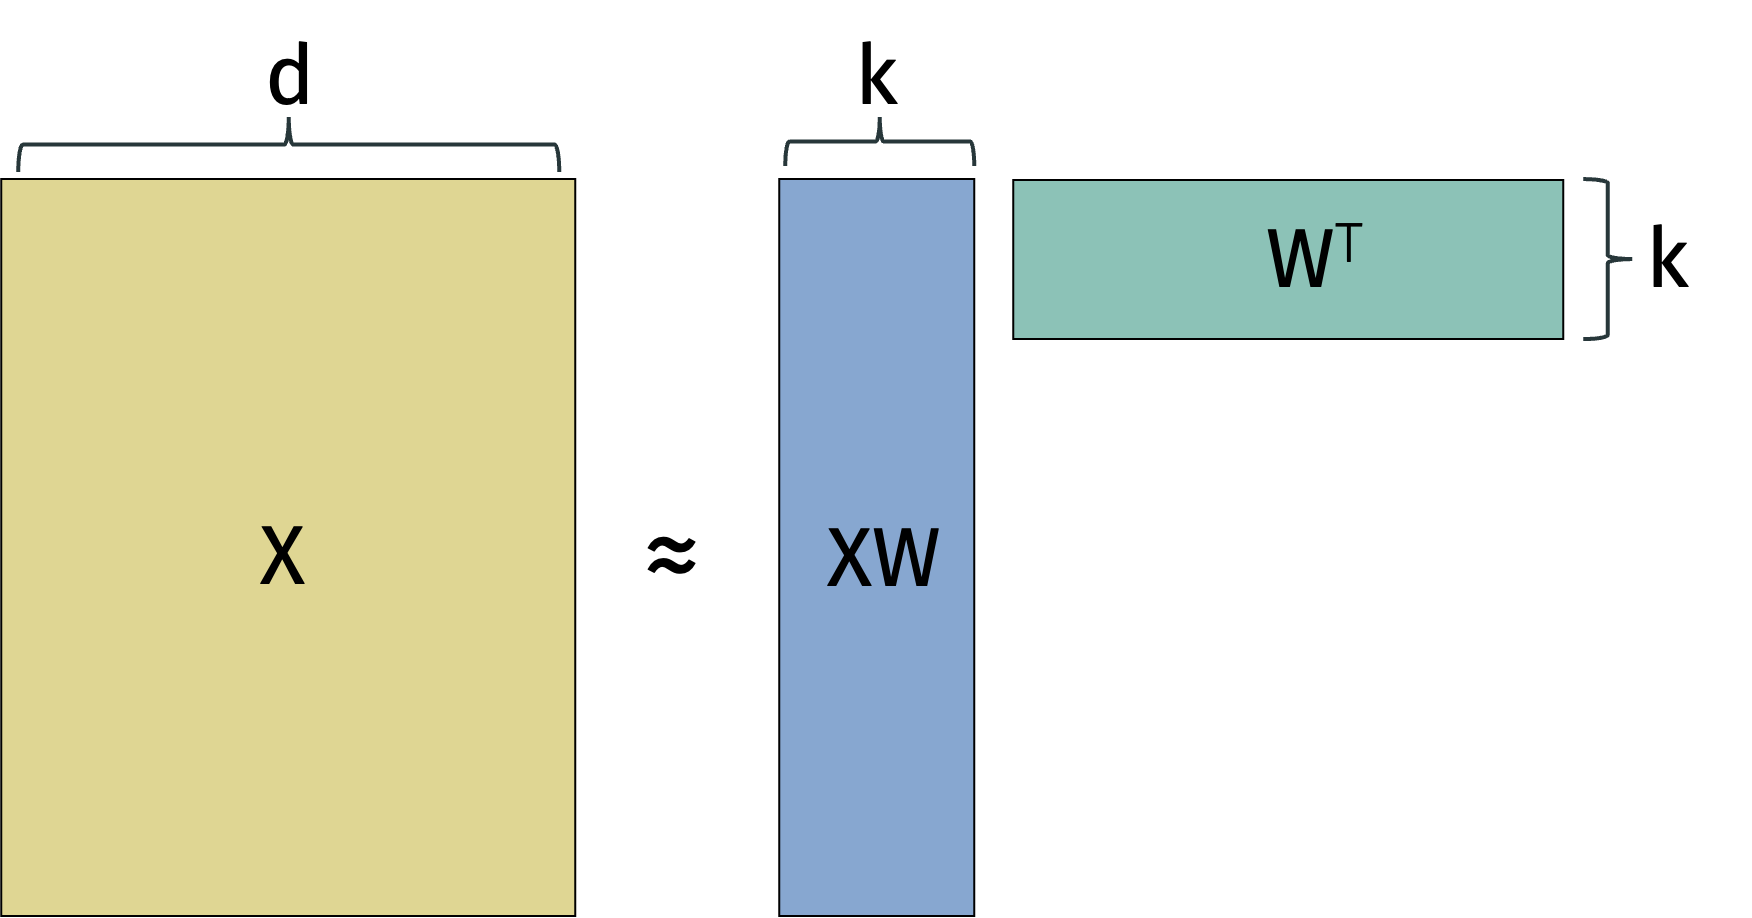
\includegraphics[width=.5\textwidth]{dualview.png}
	\end{center}
\end{frame}

\begin{frame}
	\frametitle{row redundancy}
	If a data set only had $k$ unique data points, it would be exactly rank $k$. If it has $k$ ``clusters'' of data points (e.g. the 10 digits) it's often very close to rank $k$. 
	\begin{center}
		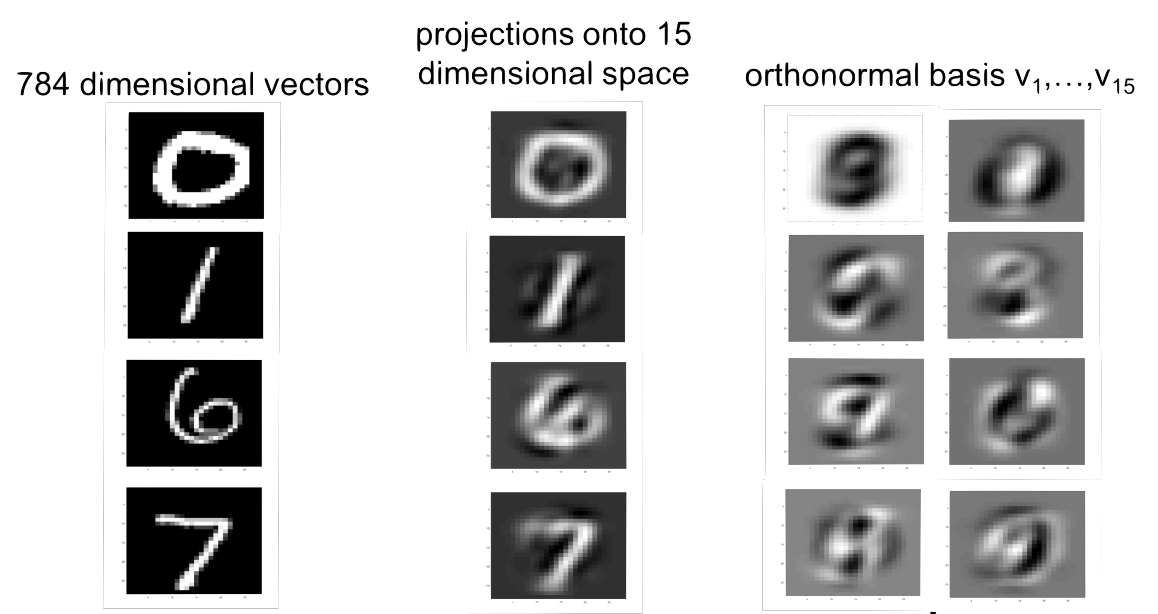
\includegraphics[width=.6\textwidth]{rowview.png}
	\end{center}
\end{frame}

\begin{frame}
	\frametitle{column redundancy}
	Colinearity/correlation of data features leads to a low-rank data matrix. 
	\begin{center}
		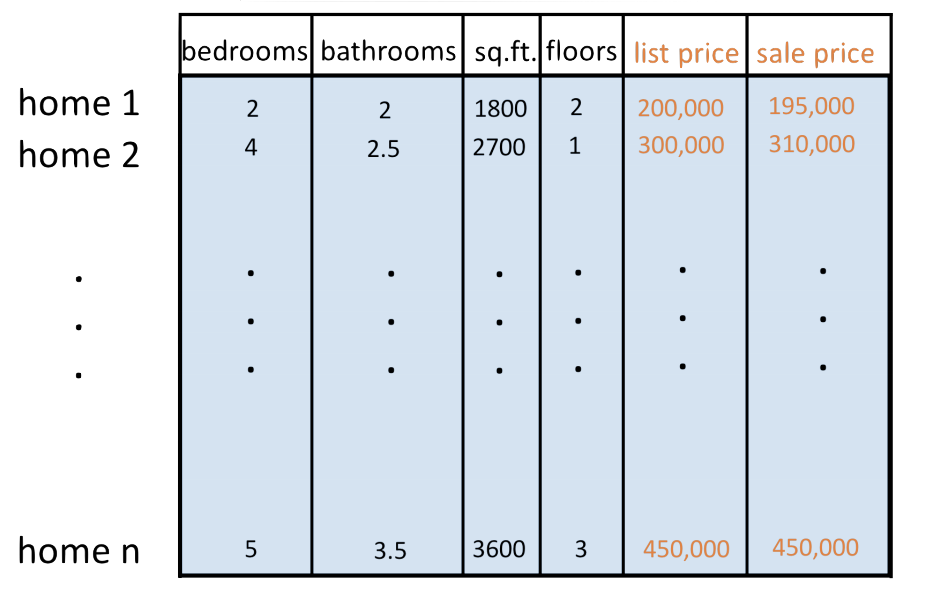
\includegraphics[width=.6\textwidth]{columnview.png}
	\end{center}
\end{frame}

\begin{frame}
	\frametitle{applications of low-rank approximation}
	Fact that $\|\bv{x}_i - \bv{x}_j\|_2 \approx \|\bv{x}_i^T\bv{WW}^T- \bv{x}_j^T\bv{WW}^T\|_2 = \|\bv{c}_i - \bv{c}_i\|_2$ leads to lots of applications.
	\begin{itemize}
		\item Data compression. E.g. used in state-of-the-art data dependent methods for nearest neighbor search.
		\item Data visualization when $k = 2$ or $3$. 
		\begin{center}
			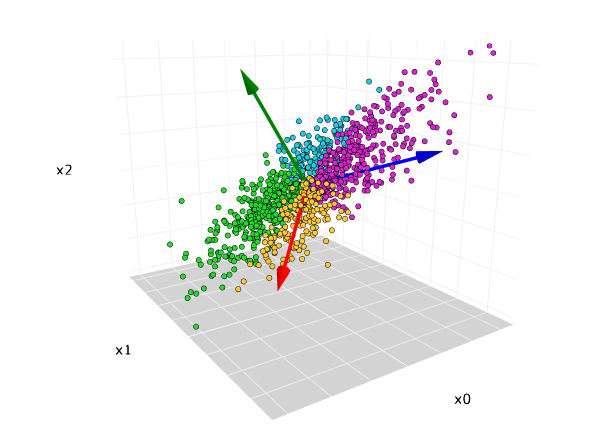
\includegraphics[width=.53\textwidth]{pca_vis.png}\hspace{1em} 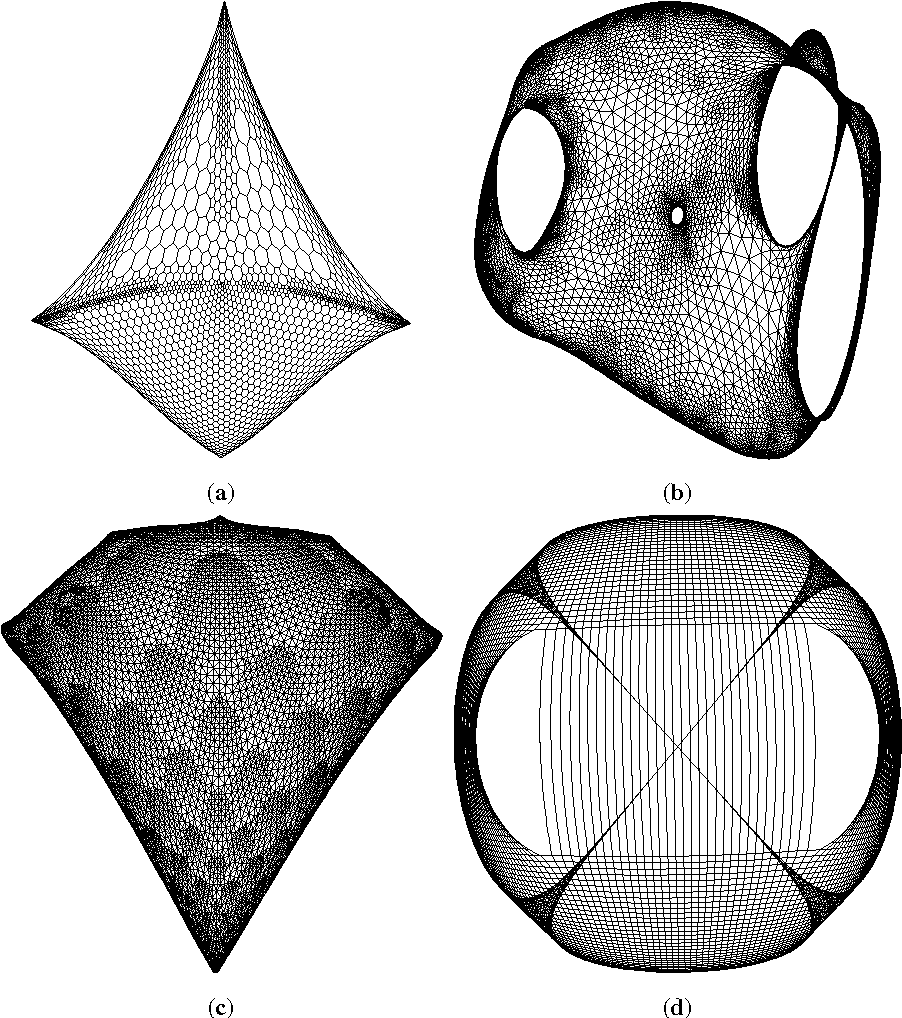
\includegraphics[width=.28\textwidth]{eigenvector_drawings.png}
		\end{center}
	\item  Data embeddings (next lecture).
	\end{itemize}
\end{frame}

\begin{frame}
	\frametitle{applications of low-rank approximation}
		\begin{itemize}
		\item Reduced order modeling for solving physical equations.
		\begin{center}
			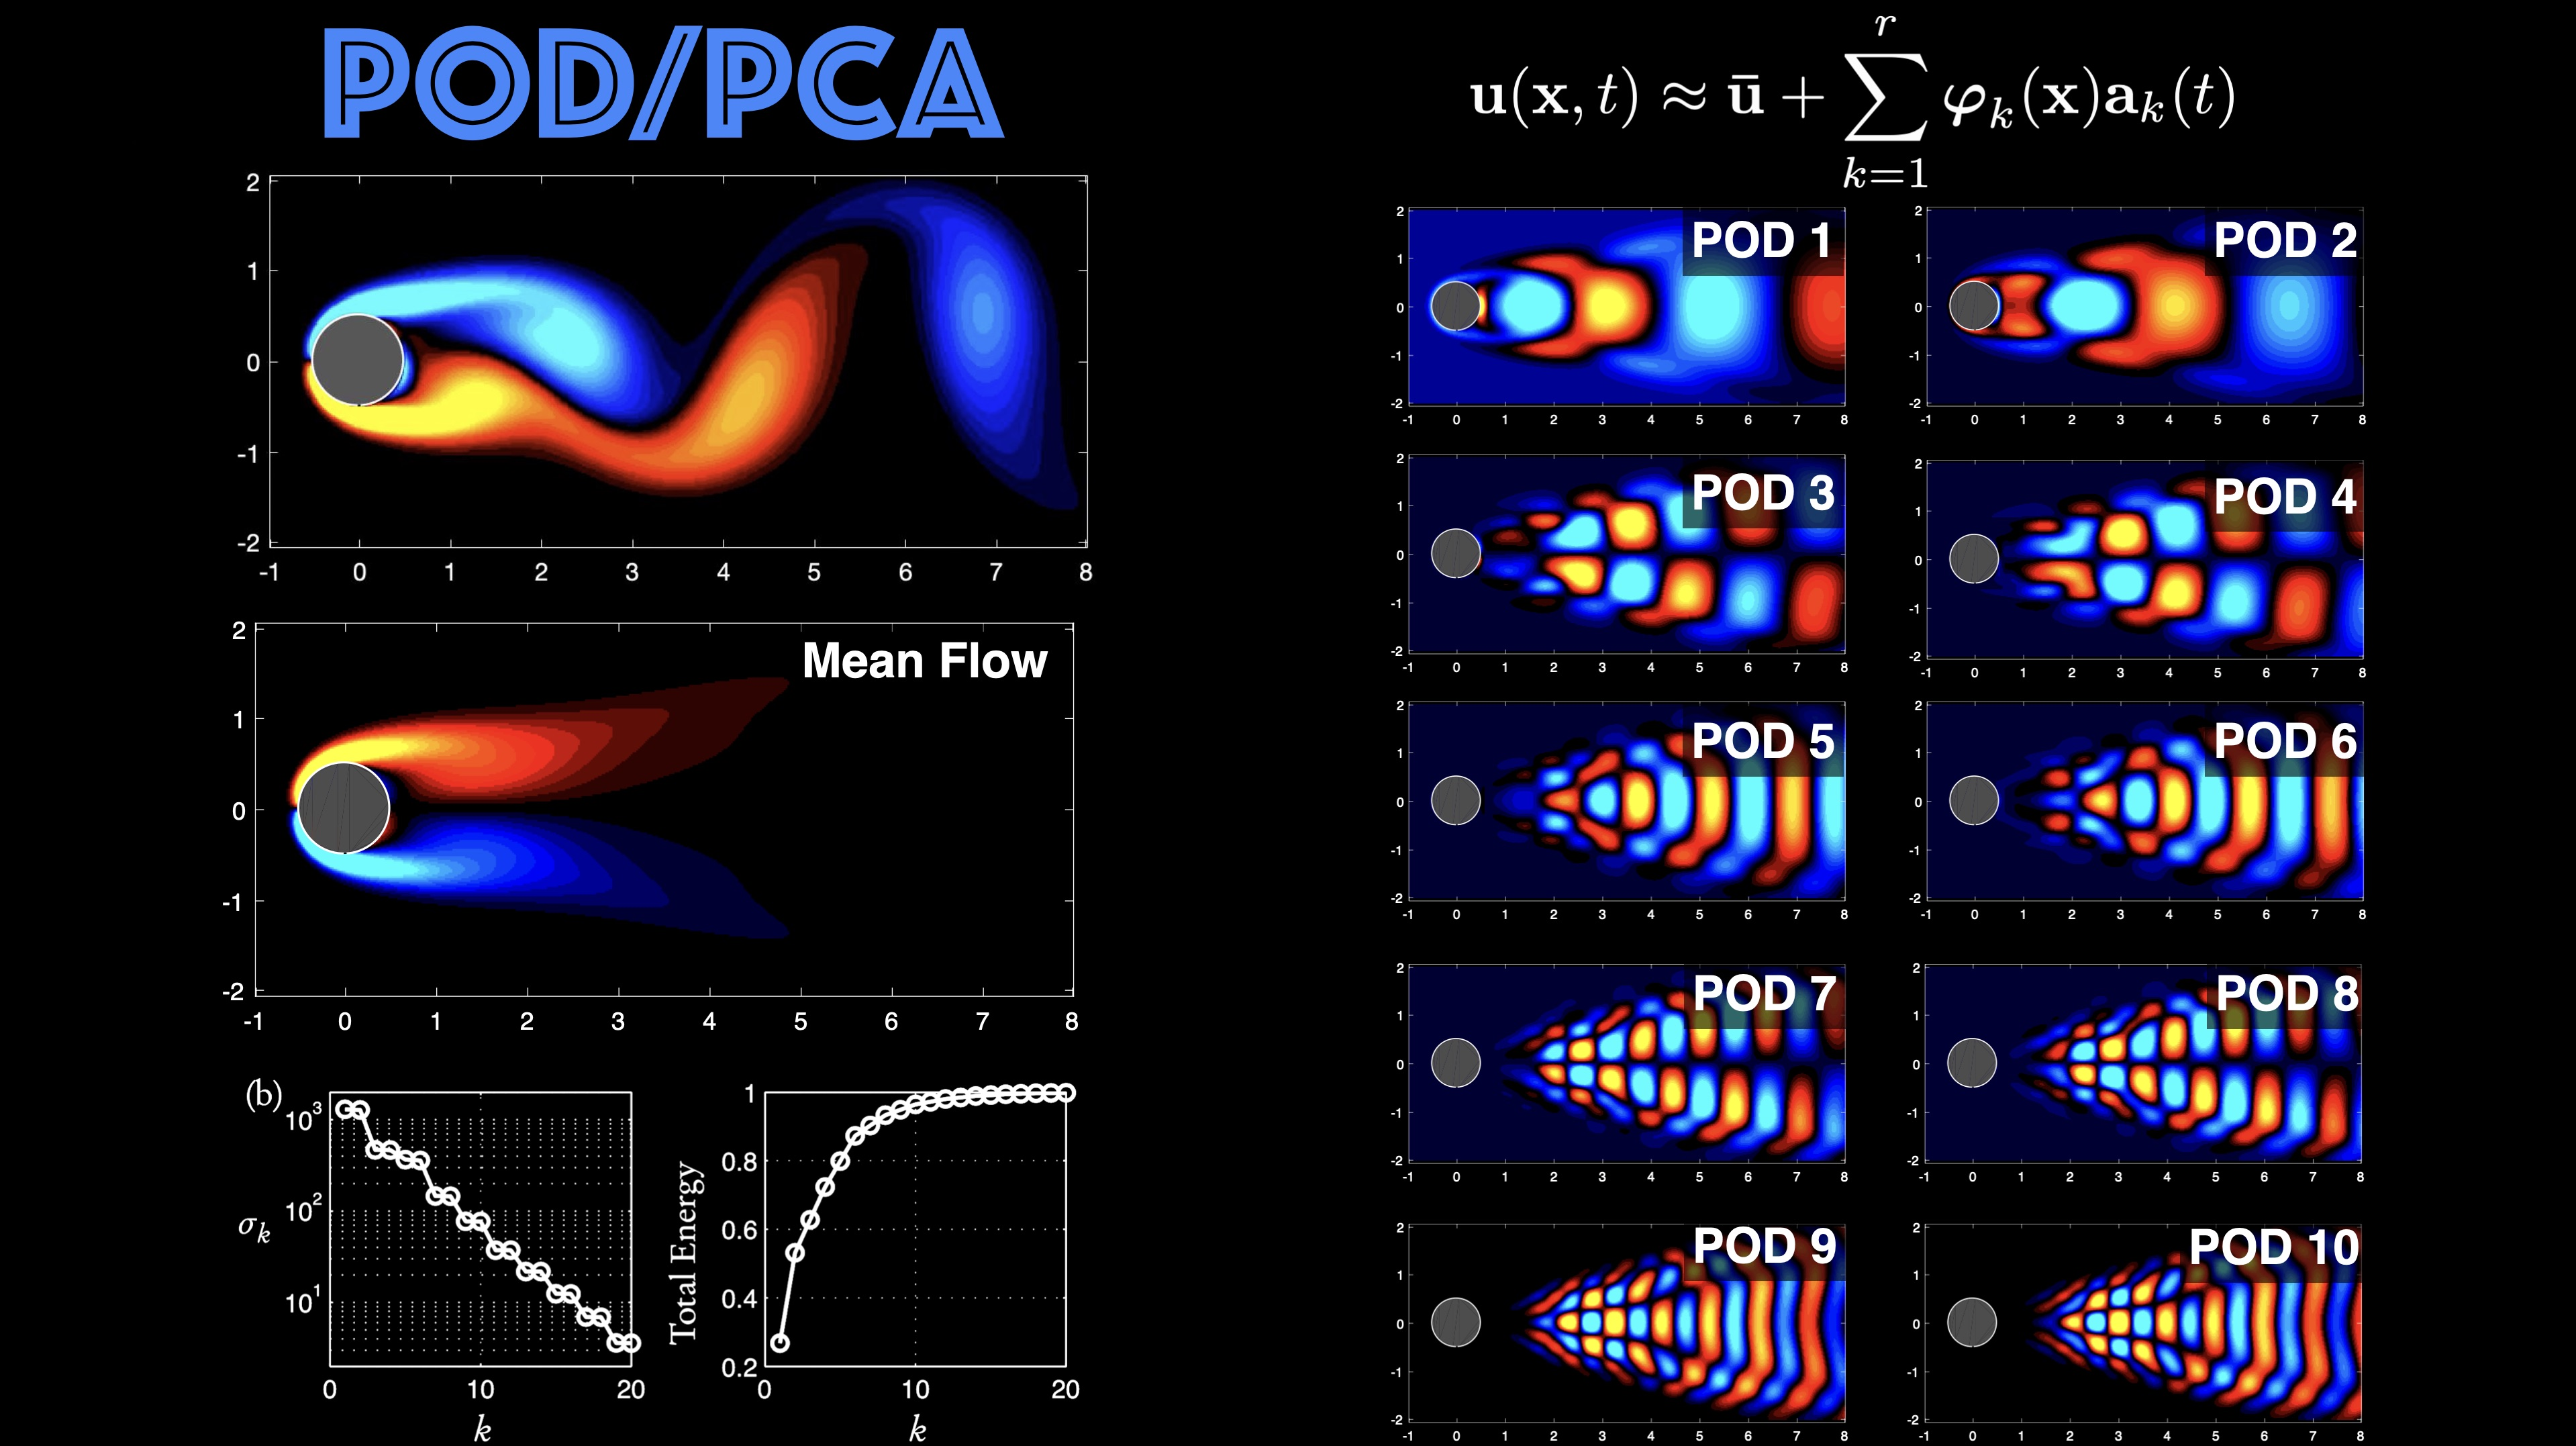
\includegraphics[width=.6\textwidth]{diffeq.jpg}
		\end{center}
		\item Constructing preconditioners in optimization.
		\item Noisy triangulation (on problem set).
	\end{itemize}
\end{frame}

\begin{frame}[t]
	\frametitle{partial svd}
	Can find the best projection from the singular value decomposition.
	\begin{center}
		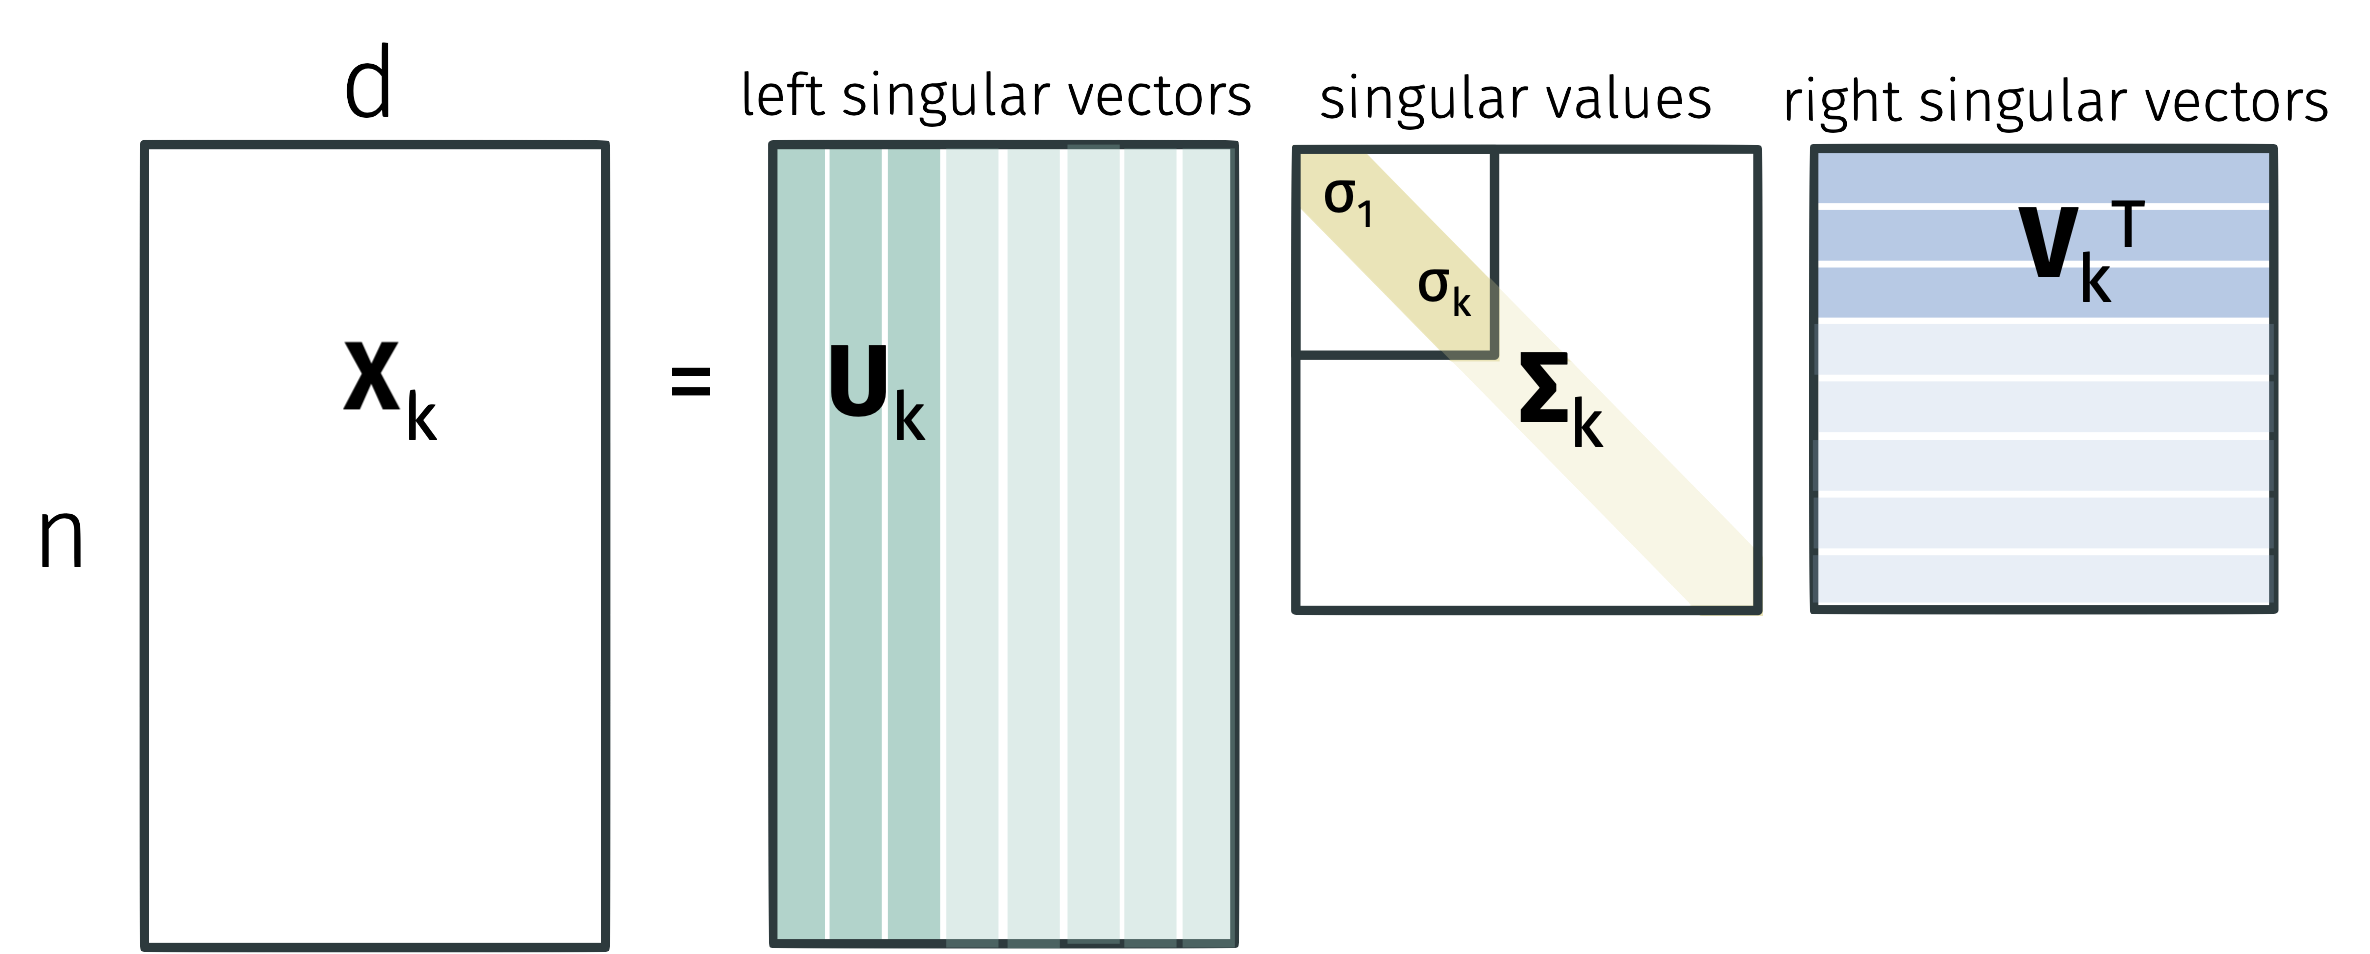
\includegraphics[width=.9\textwidth]{svdk.png}
	\end{center} 
	\begin{align*}
	\bv{V}_k = 	\argmin_{\text{orthogonal }\bv{W} \in \R^{d\times k}} \|\bv{X} - \bv{X}\bv{W}\bv{W}^T\|_F^2
%	 = \argmax_{\text{orthonormal }\bv{V} \in \R^{d\times k}} \|\bv{X}\bv{V}\bv{V}^T\|_F^2
	\end{align*}
\end{frame}

\begin{frame}[t]
	\frametitle{optimal low-rank approximation}
	\textbf{Claim:} $\bv{X}_k = \bv{U}_k\bs{\Sigma}_k\bv{V}_k^T =  \bv{X} \bv{V}_k\bv{V}_k^T$. 
\end{frame}

\begin{frame}[t]
	\frametitle{optimality of svd}
	\textbf{Claim 1:}
	\begin{align*}
		\argmin_{\text{rank $k$ }\bv{B}}  \|\bv{X} - \bv{B}|_F^2 = \bv{U}\cdot \argmin_{\text{rank $k$ }\bv{B}}   \|\bs{\Sigma}\bv{V}^T -  \bv{B}\|_F^2
	\end{align*}

		\begin{center}
	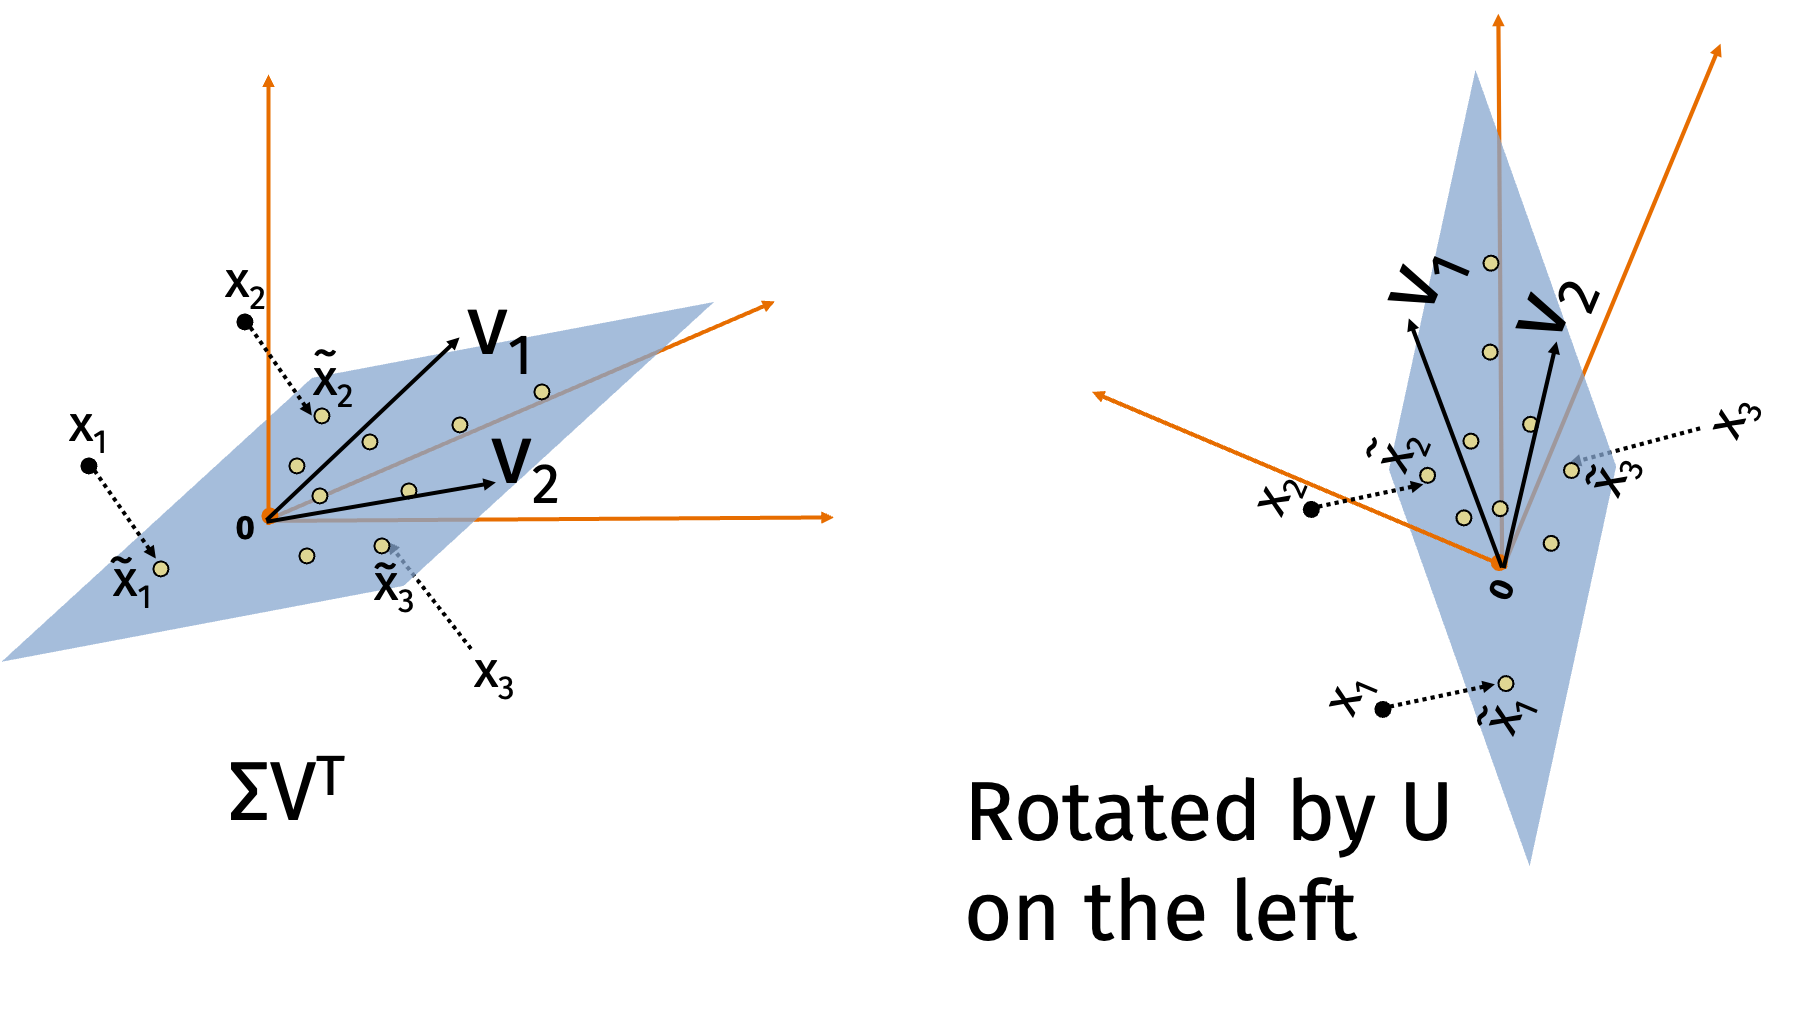
\includegraphics[width=.8\textwidth]{rotation_arg.png}
\end{center} 
\end{frame}

\begin{frame}[t]
	\frametitle{optimality of svd}	
	\textbf{Claim 2:}
	\begin{align*}
		\argmin_{\text{rank $k$ }\bv{B}}  \|\bs{\Sigma}\bv{V}^T -  \bv{B}\|_F^2 = \argmin_{\text{rank $k$ }\bv{B}}  \|\bv{V}\bs{\Sigma} -  \bv{B}^T\|_F^2
	\end{align*}
	
	\textbf{Claim 3:}
	\begin{align*}
		\argmin_{\text{rank $k$ }\bv{B}}  \|\bv{V}\bs{\Sigma} -  \bv{B}^T\|_F^2 = \argmin_{\text{rank $k$ }\bv{B}}  \|\bs{\Sigma} -  \bv{V}^T\bv{B}^T\|_F^2 
	\end{align*}

Chose $\bv{B}^T$ so that $\bv{V}^T\bv{B}^T = \bs{\Sigma}_k$.
\end{frame}

\begin{frame}[t]
	\frametitle{useful observations}
		\begin{center}
		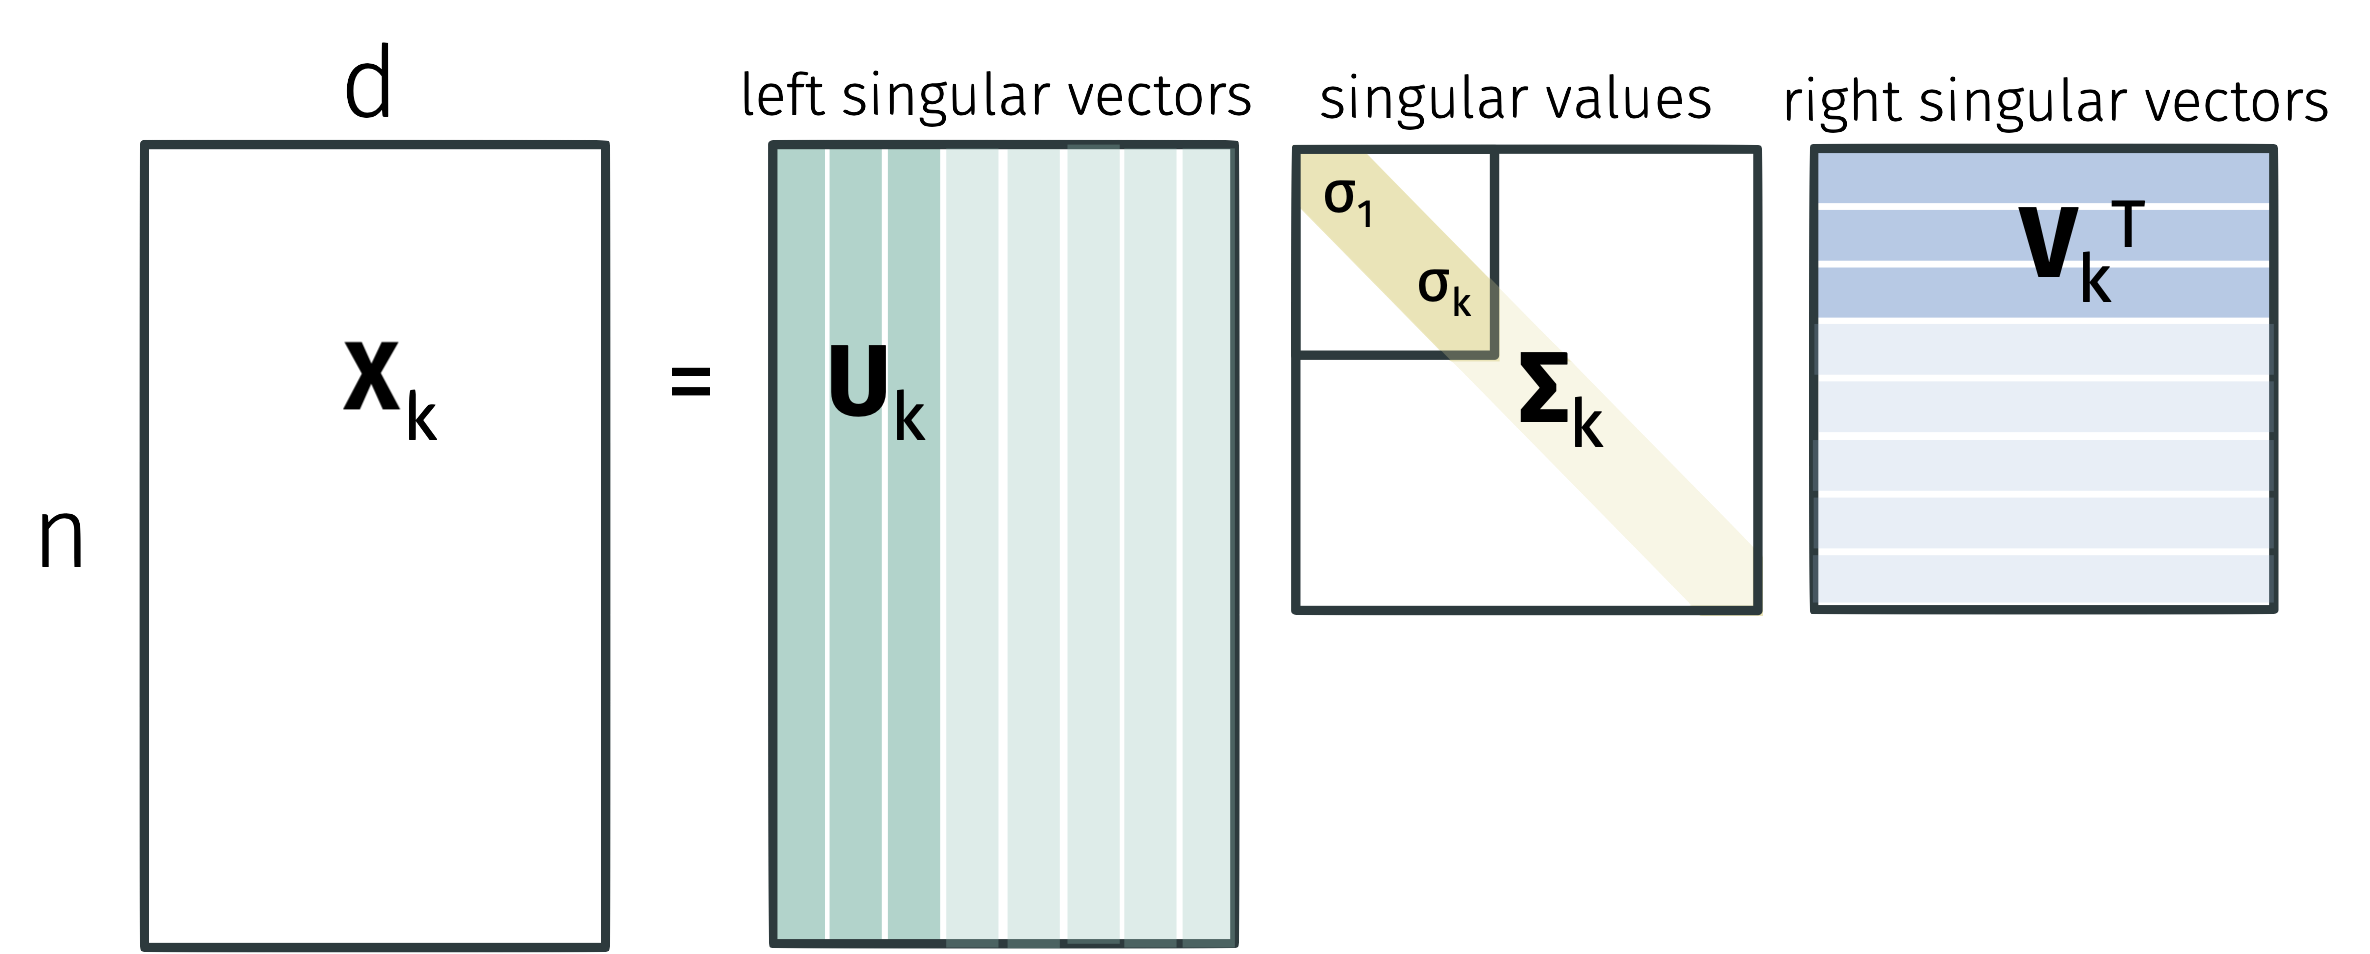
\includegraphics[width=.7\textwidth]{svdk.png}
	\end{center} 
\textbf{Observation 1:}
\begin{align*}
	\argmin_{\bv{W} \in \R^{d\times k}} \|\bv{X} - \bv{X}\bv{W}\bv{W}^T\|_F^2 = \argmax_{\bv{W} \in \R^{d\times k}} \|\bv{X}\bv{W}\bv{W}^T\|_F^2
\end{align*}
{Follows from fact that for \emph{all} orthogonal $\bv{W}$:}
\begin{align*}
	 \|\bv{X} - \bv{X}\bv{W}\bv{W}^T\|_F^2 =  \|\bv{X}\|_F^2 - \|\bv{X}\bv{W}\bv{W}^T\|_F^2
\end{align*} 
\end{frame}

\begin{frame}[t]
	\frametitle{useful observations}
	\textbf{Claim:}
	 \begin{align*}
		\|\bv{X} - \bv{X}\bv{W}\bv{W}^T\|_F^2 =  \|\bv{X}\|_F^2 - \|\bv{X}\bv{W}\bv{W}^T\|_F^2
	\end{align*} 
	\begin{center}
	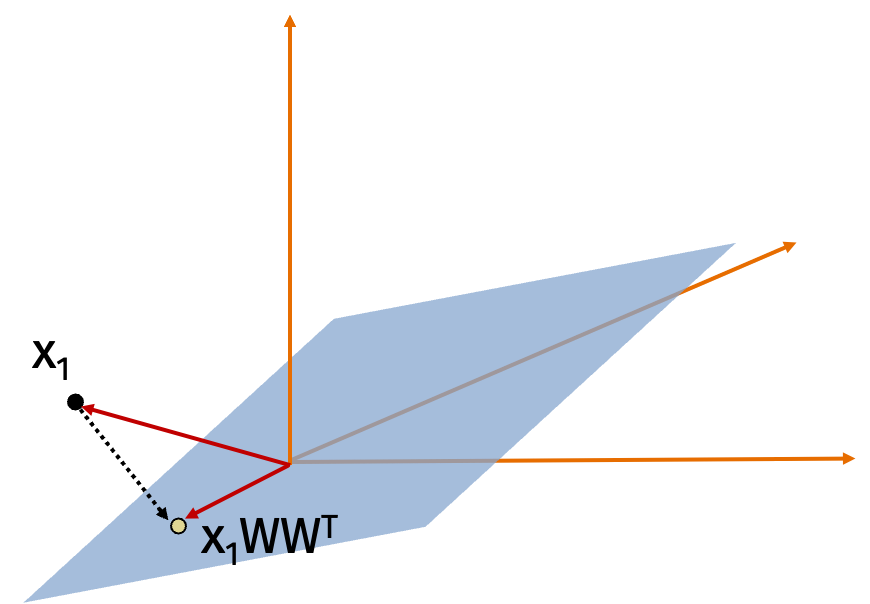
\includegraphics[width=.7\textwidth]{pythagorean.png}
\end{center} 
	
\end{frame}

\begin{frame}[t]
	\frametitle{useful observations}
	\begin{center}
		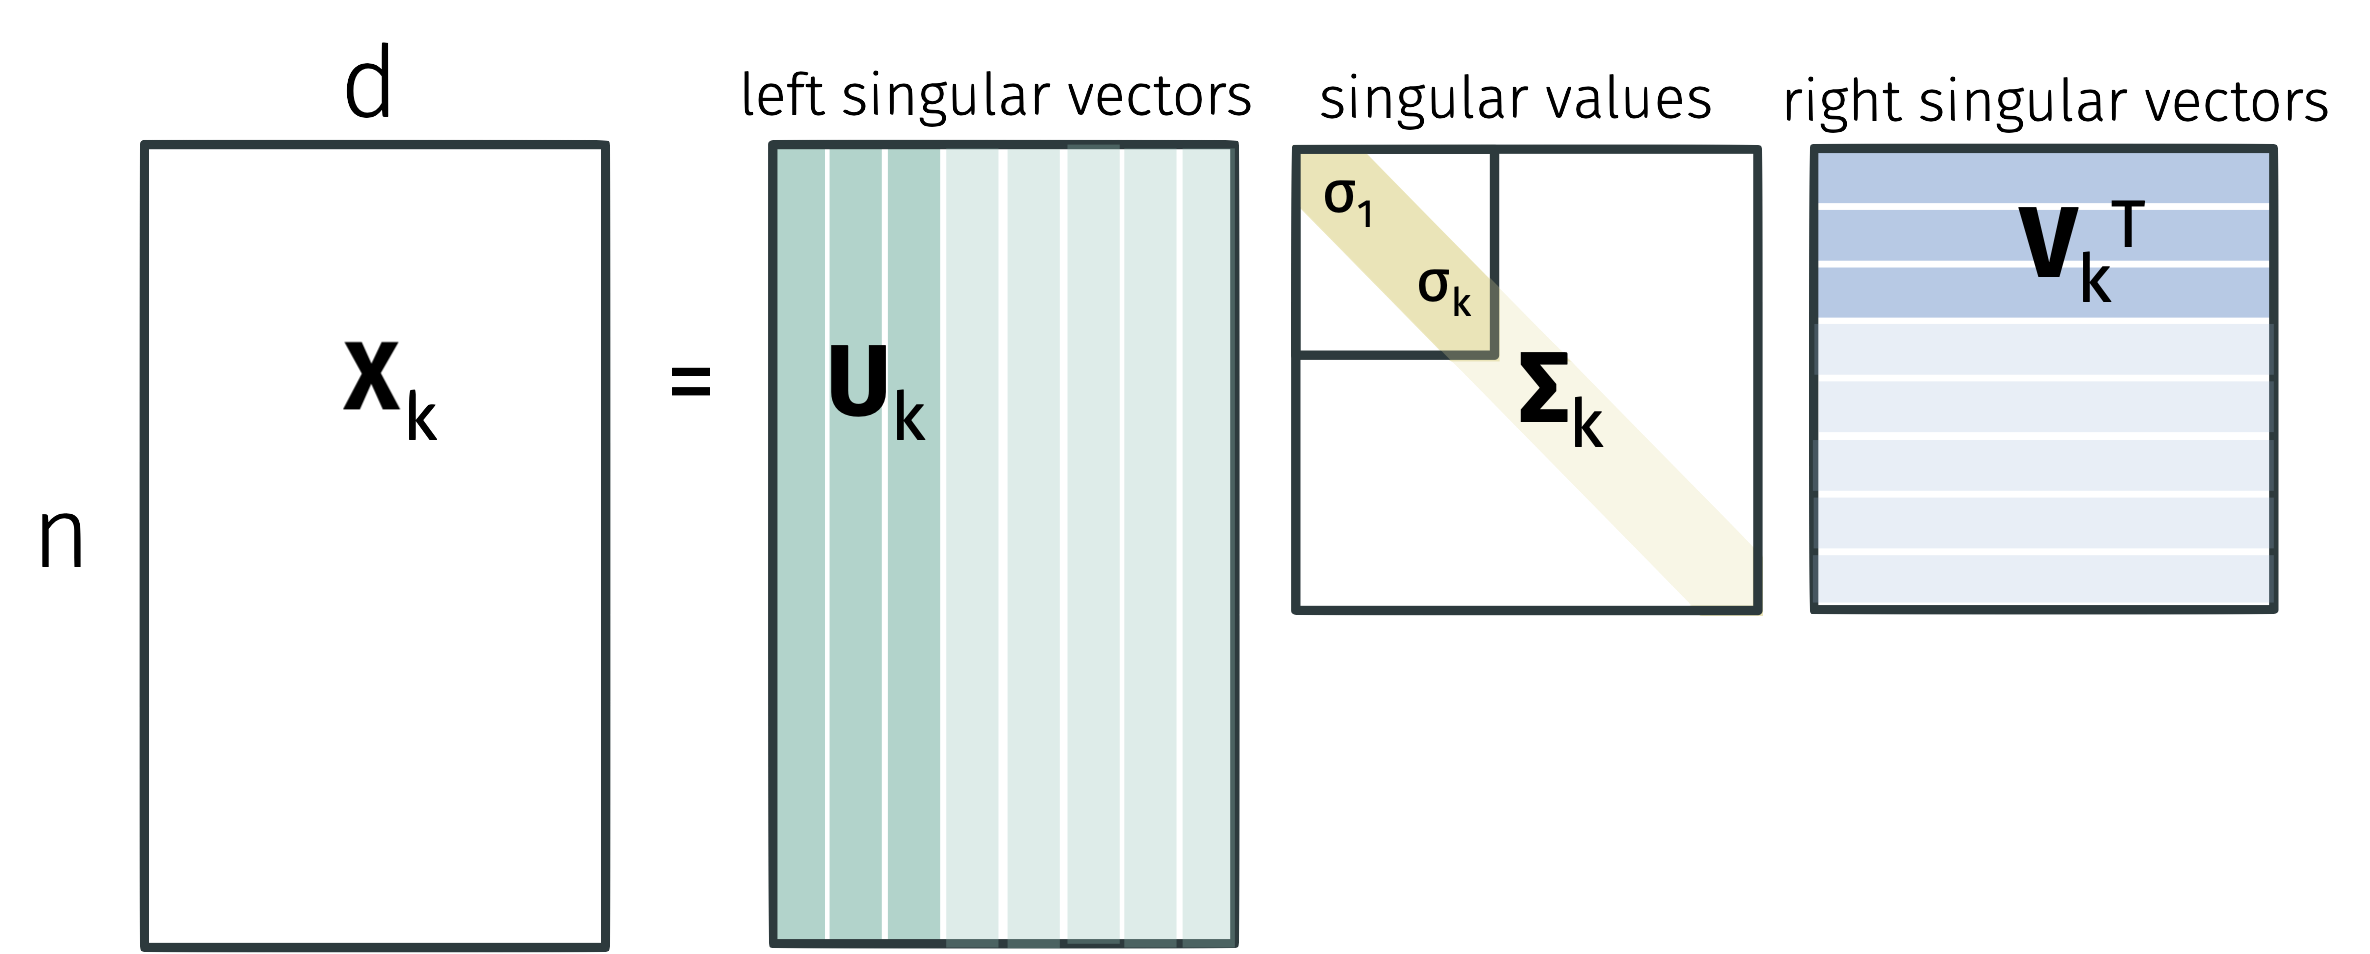
\includegraphics[width=.6\textwidth]{svdk.png}
	\end{center} 
	\textbf{Observation 2:}
	The optimal low-rank approximation error $E_k = \|\bv{X} - \bv{X}\bv{V}_k\bv{V}_k^T\|_F^2 = \|\bv{X}\|_F^2 - \|\bv{X}\bv{V}_k\bv{V}_k^T\|_F^2$ can be written:
	\begin{align*}
		E_k = \sum_{i=k+1}^d \sigma_i^2.
	\end{align*}
\end{frame}

\begin{frame}[t]
	\frametitle{spectral plots}
	\textbf{Observation 2:}
	The optimal low-rank approximation error $E_k = \|\bv{X} - \bv{X}\bv{V}_k\bv{V}_k^T\|_F^2 = \|\bv{X}\|_F^2 - \|\bv{X}\bv{V}_k\bv{V}_k^T\|_F^2$ can be written:
	\begin{align*}
	E_k = \sum_{i=k+1}^d \sigma_i^2.
	\end{align*}
	Can immediately get a sense of ``how low-rank'' a matrix is from it's spectrum:
	\begin{center}
		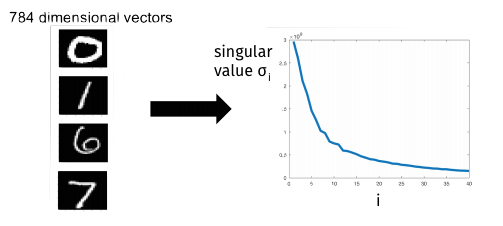
\includegraphics[width=.8\textwidth]{mnist_spectrum.png}
	\end{center}
\end{frame}

\begin{frame}[t]
	\frametitle{spectral plots}
	\textbf{Observation 2:}
	The optimal low-rank approximation error $E_k = \|\bv{X} - \bv{X}\bv{V}_k\bv{V}_k^T\|_F^2 = \|\bv{X}\|_F^2 - \|\bv{X}\bv{V}_k\bv{V}_k^T\|_F^2$ can be written:
	\begin{align*}
	E_k = \sum_{i=k+1}^d \sigma_i^2.
	\end{align*}
	Can immediately get a sense of ``how low-rank'' a matrix is from it's spectrum:
	\begin{center}
		\includegraphics[width=.8\textwidth]{noise_spectrum.png}
	\end{center}
\end{frame}

\begin{frame}[t]
	\frametitle{spectral plots}
	\textbf{Observation 2:}
	The optimal low-rank approximation error $E_k = \|\bv{X} - \bv{X}\bv{V}_k\bv{V}_k^T\|_F^2 = \|\bv{X}\|_F^2 - \|\bv{X}\bv{V}_k\bv{V}_k^T\|_F^2$ can be written:
	\begin{align*}
	E_k = \sum_{i=k+1}^d \sigma_i^2.
	\end{align*}
	Can immediately get a sense of ``how low-rank'' a matrix is from it's spectrum:
	\begin{center}
		\includegraphics[width=.8\textwidth]{cluster_spectrum.png}
	\end{center}
\end{frame}

\begin{frame}[t]
	\frametitle{computing the svd}
	Suffices to compute right singular vectors $\bv{V}$:
	\begin{itemize}
		\item Compute $\bv{X}^T\bv{X}$.
		\item Find eigendecomposition $\bv{V}\bs{\Lambda}\bv{V}^T = \bv{X}^T\bv{X}$ using e.g. QR algorithm.
		\item Compute $\bv{L} = \bv{X}\bv{V}$. Set $\sigma_i = \|\bv{L}_i\|_2$ and $\bv{U}_i = \bv{L}_i/\|\bv{L}_i\|_2$.
	\end{itemize}

\vspace{2em}
\begin{center}
	\hspace{-3em} \alert{\textbf{Total runtime $\approx$}}
\end{center}
\end{frame}

\begin{frame}[t]
	\frametitle{computing the svd (faster)}
	\textbf{Next class:}
	\begin{itemize}
		\item Compute \emph{approximate} solution.
		\item Only compute \emph{top $k$ singular vectors/values}. Runtime will depend on $k$. When $k = d$ we can't do any better than classical algorithms based on eigendecomposition.
		\item \emph{Iterative algorithms} achieve runtime $\approx O(ndk)$ vs. $O(nd^2)$ time.  
		\begin{itemize}
			\item \textbf{Krylov subspace methods} like the Lanczos method are most commonly used in practice. 
			\item \textbf{Power method} is the simplest Krylov subspace method, and still works very well. 
		\end{itemize}
	\end{itemize}
\end{frame}

% \begin{frame}[t]
% 	\frametitle{power method}
% 	\textbf{Today:} What about when $k = 1$? 
	
% 	\textbf{Goal:} Find some $\bv{z} \approx \bv{v}_1$. 
	
% 	\textbf{Input:} $\bv{X} \in \R^{n\times d}$ with SVD $\bv{U}\bs{\Sigma}\bv{V}^T$. 
% %	\textbf{Parameter:} Let $\gamma = \frac{\sigma_1 - \sigma_2}{\sigma_1}$.
	
% 	\vspace{2em}
% 	\textbf{Power method:}
% 	\begin{itemize}
% 		\item Choose $\bv{z}^{(0)}$ randomly. $\bv{z}_0 \sim \mathcal{N}(0,1)$.
% 		\item $\bv{z}^{(0)} = \bv{z}^{(0)} /\|\bv{z}^{(0)}\|_2$
% 		\item For $i = 1,\ldots, T$
% 		\begin{itemize}
% 			\item $\bv{z}^{(i)} = \bv{X}^T\cdot(\bv{X}\bv{z}^{(i-1)} )$
% 			\item $n_i = \|\bv{z}^{(i)}\|_2$
% 			\item $\bv{z}^{(i)}  = \bv{z}^{(i)} /n_i$
% 		\end{itemize}
% 	Return $\bv{z}^{(T)}$
% 	\end{itemize} 
% \end{frame}

% \begin{frame}[t]
% 	\frametitle{power method intuition}
% 	\begin{center}
% 		\includegraphics[width=\textwidth]{intuition.png}
% 	\end{center}
	
% \end{frame}

% \begin{frame}[t]
% 	\frametitle{power method formal convergence}	
% 	\begin{theorem}[Basic Power Method Convergence]
% 		Let $\gamma = \frac{\sigma_1 - \sigma_2}{\sigma_1}$ be  parameter capturing the ``gap'' between the first and second largest singular values. If Power Method is initialized with a random Gaussian vector then, with high probability, after $T = O\left(\frac{\log d/\epsilon}{\gamma}\right)$ steps, we have either:
% 		\begin{align*}
% 			\|\bv{v}_1 - \bv{z}^{(T)}\|_2 &\leq \epsilon &&\text{ or } &\|\bv{v}_1 - (-\bv{z}^{(T)})\|_2 &\leq \epsilon.
% 		\end{align*}
% 	\end{theorem}
% 	\alert{\textbf{Total runtime:}} $O\left(nd \cdot \frac{\log d/\epsilon}{\gamma}\right)$
% \end{frame}

% \begin{frame}[t]
% 	\frametitle{one step analysis of power method}
% 	Write $\bv{z}^{(i)}$ in the right singular vector basis:
% 	\begin{align*}
% 		\bv{z}^{(0)} &= c_1^{(0)}\bv{v}_1 + {c}_2^{(0)}\bv{v}_2 + \ldots + c_d^{(0)} \bv{v}_d \\
% 		\bv{z}^{(1)} &= c_1^{(1)}\bv{v}_1 + {c}_2^{(1)}\bv{v}_2 + \ldots + c_d^{(1)} \bv{v}_d\\
% 		\vdots&\\
% 		\bv{z}^{(i)} &= c_1^{(i)}\bv{v}_1 + {c}_2^{(i)}\bv{v}_2 + \ldots + c_d^{(i)} \bv{v}_d\\
% 	\end{align*}
	
% 	\textbf{Note:} $[c_1^{(i)}, \ldots, c_d^{(i)}] = \bv{c}^{(i)} = \bv{V^T}\bv{z}^{(i)}$.
	
% 	\textbf{Also:} $\|\bv{c}^{(i)}\|_2^2 = \sum_{j=1}^d \left(c_j^{(i)}\right)^2 = 1$. 
% \end{frame}

% \begin{frame}[t]
% 	\frametitle{one step analysis of power method}
% 	\textbf{Claim:} After update $\bv{z}^{(i)} =  \frac{1}{n_i}\bv{X}^T\bv{X}\bv{z}^{(i-1)}$,
% 	\begin{align*}
% 		c_j^{(i)} =  \frac{1}{n_i}\sigma_j^2 c_j^{(i-1)}
% 	\end{align*}
	
% 	\begin{align*}
% 		\bv{z}^{(i)} = \frac{1}{n_i}\left[ c_1^{(i-1)}\alert{\sigma_1^2}\cdot\bv{v}_1 + {c}_2^{(i-1)} \alert{\sigma_2^2}\cdot\bv{v}_2 + \ldots + c_d^{(i-1)} \alert{\sigma_d^2} \cdot\bv{v}_d\right]
% 	\end{align*}
% \end{frame}

% \begin{frame}[t]
% 	\frametitle{multi-step analysis of power method}
% 	\textbf{Claim:} After $T$ updates:
% 	\begin{align*}
% 	\bv{z}^{(T)} = \frac{1}{\prod_{i=1}^T n_i} \left[ c_1^{(0)}\alert{\sigma_1^{2T}}\cdot \bv{v}_1 + c_2^{(0)} \alert{\sigma_2^{2T}}\cdot \bv{v}_2 + \ldots + c_d^{(0)} \alert{\sigma_d^{2T}}\cdot \bv{v}_d \right]
% 	\end{align*}


% \vspace{10em}

% Let $\alpha_j = \frac{1}{\prod_{i=1}^T n_i}c_j^{(0)}\alert{\sigma_j^{2T}}$. 
% \textbf{Goal:} Show that $\alpha_j \ll \alpha_1$ for all $j\neq 1$. 
% \end{frame}

% \begin{frame}[t]
% 	\frametitle{power method formal convergence}	
% 	Since $\bv{z}^{(T)}$ is a unit vector, $\sum_{i=1}^d \alpha_i^2 = 1$. So $|\alpha_1| \leq 1$. 
	
% 	If we can prove that \alert{$\left| \frac{\alpha_j}{\alpha_1}\right| \leq \sqrt{\frac{\epsilon}{d}}$} then:
% 	\begin{align*}
% 		\alpha_j^2 &\leq \alpha_1^2 \cdot \frac{\epsilon}{d}\\
% 		1 = \alpha_1^2 + \sum_{j=2}^d \alpha_d^2&\leq \alpha_1^2 + \epsilon\\
% 		 \alpha_1^2 &\geq 1-\epsilon \\
% 		 \alert{|\alpha_1|} &\geq \alert{1-\epsilon}
% 	\end{align*}

% \begin{align*}
% 	\|\bv{v}_1 - \bv{z}^{(T)}\|_2 = 2 - 2\langle\bv{v}_1,\bv{z}^{(T)}\rangle \leq 2\epsilon
% \end{align*}
	
	
% \end{frame}
% \begin{frame}[t]
% 	\frametitle{power method formal convergence}
% 	Lets proves that \alert{$\left|\frac{\alpha_j}{\alpha_1}\right| \leq \sqrt{\frac{\epsilon}{d}}$} where $\alpha_j = \frac{1}{\prod_{i=1}^T n_i}c_j^{(0)}{\sigma_j^{2T}}$
	
% 	\textbf{Assumption:} Starting coefficients are all \emph{roughly} equal.
% 	\begin{align*}
% 		&\text{For all $j$} & O(1/d^{1.5}) &\leq \left| c_j^{(0)}\right| \leq 1. 
% 	\end{align*}
% 	This is a very loose bound, but it's all that we will need. We will prove shortly that it holds with probability $99/100$.
	
% 	\begin{align*}
% 		\frac{|\alpha_j|}{|\alpha_1|} = \frac{\sigma_j^{2T}}{\sigma_1^{2T}} \cdot \frac{|c_j^{(0)}|}{|c_1^{(0)}|} \leq \hspace{20em}
% 	\end{align*}
	
% 	\begin{align*}
% 		\text{Need } T = \hspace{10em}
% 	\end{align*}
% \end{frame}

% \begin{frame}[t]
% 		\frametitle{starting coefficient analysis}
% 	\textbf{Need to prove:} Starting coefficients are all \emph{roughly} equal.
% 	\begin{align*}
% 		&\text{For all $j$} & O(1/d^{1.5}) &\leq |c_j^{(0)}| \leq 1 
% 	\end{align*}
% 	with probability $99/100$. \textbf{Prove using Gaussian (anti)-concentration.}
	
% 	Right hand side is immediate from fact that $\sum_j (c_j^{(0)})^2 = 1$.	
	
% 	To show the left hand side we first use rotational invariance of Gaussian:
% 	\vspace{-.5em}
% 	\begin{align*}
% 		\bv{c}^{(0)} = \frac{\bv{V}^T \bv{z}^{(0)}}{\| \bv{z}^{(0)}\|_2} =  \frac{\bv{V}^T \bv{z}^{(0)}}{\| \bv{V}^T\bv{z}^{(0)}\|_2} \sim \frac{\bv{g}}{\| \bv{g}\|_2}, 
% 	\end{align*}
% 	where $\bv{g} \sim \mathcal{N}(0,1)^d$.
% \end{frame}

% \begin{frame}[t]
% 	\frametitle{starting coefficient analysis}
% 	Need to show that with high probability, every entry of $\frac{\bv{g}}{\| \bv{g}\|_2} \geq c\cdot \frac{1}{d^{1.5}}$. 
	
% 	\textbf{Part 1:}
% 	With probablility $999/100$, 
% 	\begin{align*}
% 		\|\bv{g}\|_2^2 \leq 
% 	\end{align*}
% \end{frame}

% \begin{frame}[t]
% 	\frametitle{starting coefficient analysis}
% 	Need to show that with high probability, the magnitude of every entry of ${\bv{g}} \geq c\cdot \frac{1}{d}$. 
	
% 	\textbf{Part 2:}
% 	With probablility $1 - c/d$, 
% 	\begin{align*}
% 		\min_i |{g}_i| \geq  O\left(\frac{c}{d}\right).
% 	\end{align*}
% \vspace{-1em}

% 	\begin{center}
% 		\includegraphics[width=.6\textwidth]{basic_gauss.png}
% 	\end{center}
% Applying union bound completes the result.
% \end{frame}

% \begin{frame}[t]
% 	\frametitle{power method formal convergence}	
% 	\begin{theorem}[Basic Power Method Convergence]
% 		Let $\gamma = \frac{\sigma_1 - \sigma_2}{\sigma_1}$ be  parameter capturing the ``gap'' between the first and second largest singular values. If Power Method is initialized with a random Gaussian vector then, with high probability, after $T = O\left(\frac{\log d/\epsilon}{\gamma}\right)$ steps, we have either:
% 		\begin{align*}
% 			\|\bv{v}_1 - \bv{z}^{(T)}\|_2 &\leq \epsilon &&\text{ or } &\|\bv{v}_1 - (-\bv{z}^{(T)})\|_2 &\leq \epsilon.
% 		\end{align*}
% 	\end{theorem}
% 	The method truly won't converge if $\gamma$ is very small. Consider extreme case when $\gamma = 0$.
% 	\begin{align*}
% 		\bv{z}^{(T)} = \frac{1}{\prod_{i=1}^T n_i} \left[ c_1^{(0)}\alert{\sigma_1^{2T}}\cdot \bv{v}_1 + c_2^{(0)} \alert{\sigma_2^{2T}}\cdot \bv{v}_2 + \ldots + c_d^{(0)} \alert{\sigma_d^{2T}}\cdot \bv{v}_d \right]
% 	\end{align*}
% \end{frame}

% \begin{frame}[t]
% 	\frametitle{power method -- no gap dependence}	
% 	\begin{theorem}[Gapless Power Method Convergence]
% 		 If Power Method is initialized with a random Gaussian vector then, with high probability, after $T = O\left(\frac{\log d/\epsilon}{\epsilon}\right)$ steps, we obtain a $\bv{z}$ satisfying:
% 		\begin{align*}
% 		\|\bv{X} - \bv{X}\bv{z}\bv{z}^{T}\|_F^2 \leq (1+\epsilon)\|\bv{X} - \bv{X}\bv{v}_1\bv{v}_1^T\|_F^2 
% 		\end{align*}
% 	\end{theorem}	
% \textbf{Intuition:} For a good low-rank approximation, we don't actually need to converge to $\bv{v}_1$ if $\sigma_1$ and $\sigma_2$ are the same or very close. Would suffice to return either $\bv{v}_1$ or $\bv{v}_2$, or some linear combination of the two.
% \end{frame}

% \begin{frame}[t]
% 	\frametitle{generalizations to larger $k$}
% 	\begin{itemize}
% 		\item Block Power Method aka Simultaneous Iteration aka Subspace Iteration aka Orthogonal Iteration
% 	\end{itemize}
% 	\textbf{Power method:}
% \begin{itemize}
% 	\item Choose $\bv{G}\in \R^{d\times k}$ be a random Gaussian matrix. 
% 	\item $\bv{Z}_0 = \orth(\bv{G})$.
% 	\item For $i = 1,\ldots, T$
% 	\begin{itemize}
% 		\item $\bv{Z}^{(i)} = \bv{X}^T\cdot(\bv{X}\bv{Z}^{(i-1)} )$
% 		\item $\bv{Z}^{(i)}  = \orth(\bv{Z}^{(i)})$
% 	\end{itemize}
% 	Return $\bv{Z}^{(T)}$
% \end{itemize}
	
% 	\begin{center}
% 		\alert{\textbf{Runtime}:} $O\left(\frac{\log d/\epsilon}{\epsilon}\right)$iterations to obtain a nearly optimal low-rank approximation:
% 		\begin{align*}
% 			\|\bv{X} - \bv{X}\bv{Z}\bv{Z}^T\|_F^2 \leq (1+\epsilon)\|\bv{X} - \bv{X}\bv{V_k}\bv{V_k}^T\|_F^2.
% 		\end{align*}
% 	\end{center}
% \end{frame}

% \begin{frame}[t]
% 	\frametitle{krylov methods}
% 	Possible to ``accelerate'' these methods. 
	
% 	\begin{center}
% 		\alert{\textbf{Convergence Guarantee}:} $T = O\left(\frac{\log d/\epsilon}{\alert{\sqrt{\epsilon}}}\right)$ iterations to obtain a nearly optimal low-rank approximation:
% 		\begin{align*}
% 			\|\bv{X} - \bv{X}\bv{Z}\bv{Z}^T\|_F^2 \leq (1+\epsilon)\|\bv{X} - \bv{X}\bv{V_k}\bv{V_k}^T\|_F^2.
% 		\end{align*}
		
% 		\textbf{Runtime}: ${O}(\nnz(\bv{X})\cdot k \cdot T) \leq {O}(ndk \cdot T)$.
% 	\end{center}
% \end{frame}

% \begin{frame}[t]
% 	\frametitle{krylov subspace methods}
% 	\begin{align*}
% 		\bv{z}^{(q)} = c \cdot \left(\bv{X}^T\bv{X}\right)^q \cdot \bv{g}
% 	\end{align*}
% 	\begin{center}
% 		\includegraphics[width=.5\textwidth]{basic_jump.png}
% 	\end{center}
% 	\begin{align*}
% 		\bv{z}^{(q)}  = c\cdot \left[c_1 \cdot \sigma_1^{2q} \bv{v}_1 + c_2 \cdot \sigma_2^{2q} \bv{v}_2 + \ldots + c_n \cdot \sigma_n^{2q} \bv{v}_n   \right]
% 	\end{align*}
% \end{frame}	

% \begin{frame}[t]
% 	\frametitle{krylov subspace methods}
% 	\begin{align*}
% 		\bv{z}^{(q)} = c \cdot \left(\bv{X}^T\bv{X}\right)^q \cdot \bv{g}
% 	\end{align*}
% 	Along the way we computed:
% 	\begin{align*}
% 		\mathcal{K}_q = \left[\bv{g}, \left(\bv{X}^T\bv{X}\right) \cdot \bv{g}, \left(\bv{X}^T\bv{X}\right)^2 \cdot \bv{g}, \ldots, \left(\bv{X}^T\bv{X}\right)^q \cdot \bv{g}\right]
% 	\end{align*}
% 	$\mathcal{K}$ is called the  \emph{Krylov subspace of degree $q$}. 
	
% 	\vspace{2em}
% 	\textbf{Idea behind Krlyov methods:} Don't throw away everything before $\left(\bv{X}^T\bv{X}\right)^q \cdot \bv{g}$. What you're using when you run \texttt{svds} or \texttt{eigs} in MATLAB or Python.
% \end{frame}

% \begin{frame}[t]
% 	\frametitle{krylov subspace methods}
% 	\begin{center}
% 		Want to find $\bv{v}$, which minimizes $\|\bv{X} - \bv{X}\bv{v}\bv{v}^T\|_F^2$.
% 	\end{center}
	
% 	\textbf{Lanczos method:}
% 	\begin{itemize}
% 		\item Let $\bv{Q} \in \R^{d\times k}$ be an orthonormal span for the vectors in $\mathcal{K}$. 
% 		\item Solve $\min_{\bv{v} = \bv{Q}\bv{w}} \|\bv{X} - \bv{X}\bv{v}\bv{v}^T\|_F^2$. 
% 		\begin{itemize}
% 			\item Find \emph{best} vector in the Krylov subspace, instead of just using last vector.
% 			\item Can be done in $O\left(ndk + dk^2\right)$ time. 
% 		\end{itemize}
% 	\end{itemize}
% \end{frame}

% \begin{frame}[t]
% 	\frametitle{lanczos method analysis}
% 	For a degree $t$ polynomial $p$, let $\bv{v}_p = \frac{p(\bv{X}^T\bv{X})\bv{g}}{\|p(\bv{X}^T\bv{X})\bv{g}\|_2}$.
		
% 	Power method returns:
% 	\begin{align*}
% 		\bv{v}_{x^t}.
% 	\end{align*}

% 	Lanczos method returns 	$\bv{v}_{p^*}$ where:
% 	\begin{align*}
% 		p^* = \argmin_{\text{degree $t$ } p} \|\bv{X} - \bv{X}\bv{v}_p\bv{v}_p^T\|_F^2.
% 	\end{align*}
% \end{frame}

% %\begin{frame}[t]
% %	\frametitle{lanczos method analysis}
% %	\textbf{Claim 1:} For any degree $q$ polynomial $p$, we can write $p(\bv{X}^T\bv{X})\cdot \bv{g}$ as $\bv{Q}\bv{w}$ for some $\bv{w}$.
% %	
% %	\vspace{2em}
% %	\textbf{Claim 2:} 
% %	\begin{align*}
% %		\min_{\bv{v} = \bv{Q}\bv{w}} \|\bv{X} - \bv{X}\bv{v}\bv{v}^T\|_F^2 = \min_{\text{degree $q$ polynomial} p} \|\bv{X} - \bv{X}\bv{v}_p\bv{v}_p^T\|_F^2
% %	\end{align*}
% %	where $\bv{v}_p = p(\bv{X}^T\bv{X})\cdot \bv{g}$. 
% %	
% %	\vspace{2em}
% %	\textbf{Claim 3:} 
% %	\begin{align*}
% %		\bv{z}^{(q)}  = c\cdot \left[c_1 \cdot p(\sigma_1^{2}) \bv{v}_1 + c_2 \cdot p(\sigma_2^{2}) \bv{v}_2 + \ldots + c_n \cdot p(\sigma_n^{2}) \bv{v}_n   \right]
% %	\end{align*}
% %	
% %	{}\end{frame}
% %
% \begin{frame}[t]
% 	\frametitle{lanczos method analysis}
% 	\textbf{Claim:} There is a $t = O\left(\sqrt{q\log\frac{1}{\Delta}}\right)$degree polynomial $\hat{p}$ approximating $\bv{x}^q$ up to error $\Delta\sigma_1^2$ on $[0,\sigma_1^2]$.
% 	\begin{center}
% 		\includegraphics[width=.4\textwidth]{basic_jump.png} 
% 	\end{center}
	
% 	$\|\bv{X} - \bv{X}\bv{v}_{{p}^*}\bv{v}_{{p}^*}^T\|_F^2 \leq \|\bv{X} - \bv{X}\bv{v}_{\hat{p}}\bv{v}_{\hat{p}}^T\|_F^2 \approx \|\bv{X} - \bv{X}\bv{v}_{x^q}\bv{v}_{x^q}^T\|_F^2 \approx \|\bv{X} - \bv{X}\bv{v}_1\bv{v}_1^{T}\|_F^2$
	
% 	\textbf{\alert{Runtime}:} $O\left(\frac{\log(d/\epsilon)}{\sqrt{\gamma}} \cdot \nnz(\bv{X})\right)$ vs. $O\left({\frac{\log(d/\epsilon)}{\gamma}} \cdot \nnz(\bv{X})\right)$ 
% \end{frame}

% \begin{frame}[t]
% 	\frametitle{power method -- no gap dependence}	
% 	Again convergence is slow when $\gamma = \frac{\sigma_1 - \sigma_2}{\sigma_1}$ is small. $\bv{z}^{(q)}$ has large components of \emph{both} $\bv{v}_1$ and $\bv{v}_2$. But in this case:
	
% 	\begin{align*}
% 		\|\bv{X} - \bv{X}\bv{v}_1\bv{v}_1^T\|_F^2 = \sum_{i\neq 1} \sigma_i^2 \approx  \sum_{i\neq 2} = \sigma_i^2 \|\bv{X} - \bv{X}\bv{v}_2\bv{v}_2^T\|_F^2.
% 	\end{align*}
	
% 	\begin{center}
% 		\alert{So we don't care! Either $\bv{v}_1$ or $\bv{v}_2$ give good rank-$1$ approximations.}
% 	\end{center}
	
% 	\textbf{Claim}: To achieve
% 	\begin{align*}
% 		\|\bv{X} - \bv{X}\bv{z}\bv{z}^{T}\|_F^2 \leq (1+\epsilon)\|\bv{X} - \bv{X}\bv{v}_1\bv{v}_1^T\|_F^2 
% 	\end{align*}
% 	we need $O\left(\frac{\log(d/\epsilon)}{\epsilon} \right)$ 
% 	power method iterations or $O\left(\frac{\log(d/\epsilon)}{\sqrt{\epsilon}} \right)$ Lanczos iterations.
% \end{frame}

% \begin{frame}[t]
% 	\frametitle{generalizations to larger $k$}
% 	\begin{itemize}
% 		\item Block Krylov methods
% 	\end{itemize}
	
% 	\begin{itemize}
% 		\item Let $\bv{G}\in \R^{d\times k}$ be a random Gaussian matrix.
% 		\item  $\mathcal{K}_q = \left[\bv{G}, \left(\bv{X}^T\bv{X}\right) \cdot \bv{G}, \left(\bv{X}^T\bv{X}\right)^2 \cdot \bv{G}, \ldots, \left(\bv{X}^T\bv{X}\right)^q \cdot \bv{G}\right]$
% 	\end{itemize}
	
% 	\begin{center}
% 		\alert{\textbf{Runtime}:} $O\left(\nnz(\bv{X}) \cdot k \cdot \frac{\log d/\epsilon}{\sqrt{\epsilon}}\right)$ to obtain a nearly optimal low-rank approximation.
% 	\end{center}
% \end{frame}


\end{document} 




